% Autor: Alfredo Sánchez Alberca (asalber@ceu.es)
%!TEX program = latex
% ASPECT RATIO FOR YOUTUBE VIDEO
%\documentclass[aspectratio=1610,mathserif,profesionalfont,10pt,dvips,blue,xcolor=table]{beamer}
% ASPECT RATIO FOR PROJECTOR
%\documentclass[mathserif,profesionalfont,10pt,dvips,blue,xcolor=table]{beamer} 
% ARTICLE VERSION 
\documentclass[10pt,a4paper,titlepage]{article} \usepackage{beamerarticle}  

\usepackage{pxfonts}
%\usepackage{lucidaso}
%\usepackage{eulervm}
%\usepackage{mathpazo}
%\renewcommand{\rmdefault}{ibh}
\setbeamersize{text margin left=.5cm, text margin right=.5cm}

%\usetheme[width=0pt,height=20pt,hideallsubsections]{PaloAlto}
%\useoutertheme[width=0pt,height=30pt,hideallsubsections]{sidebar}
\useoutertheme{default}
\useinnertheme[shadow]{rounded}
%\useoutertheme{shadow}
%\usecolortheme[named=red]{structure}
%\useinnertheme[shadow]{rounded}
%\usecolortheme{sidebartab}
%\usecolortheme[overlystylish]{albatross}
%\usecolortheme{crane} 
%\usecolortheme{lily}
\usecolortheme{whale}
\usecolortheme{rose} 
%\setbeamercovered{transparent}

%\beamertemplateshadingbackground{blue!10}{yellow!10} 

% REMOVE NAVIGATIONS SYMBOLS
\setbeamertemplate{navigation symbols}{}

% ITEM BULLETS 
\setbeamertemplate{itemize items}[default]
\setbeamertemplate{enumerate items}[default]

\setbeamertemplate{section in toc}[sections numbered]
\setbeamertemplate{subsection in toc}[subsections numbered]

% HANDOUTS
% \setbeameroption{show notes}
% \setbeamertemplate{note page}[plain]
% \setbeamerfont{note page}{size=\scriptsize}

% FOOT
\setbeamertemplate{footline}[split]
% \vbox{%
% \tinycolouredline{structure}{\color{white}\textbf{Curso B\'asico de Estad\'istica \hfill%
% \insertshortinstitute\hfill
% \insertframenumber{} / \inserttotalframenumber
% }}%
% }}

\usepackage[utf8]{inputenc}
\usepackage{amsmath}
\usepackage{amsfonts}
\usepackage{amssymb}
\usepackage{array}
\usepackage{multirow}
\usepackage{textcomp}
\usepackage[usenames,dvipsnames]{pstricks}
\usepackage{pst-all,pst-math,pst-plot,pst-infixplot,pst-xkey,pstricks-add}
\usepackage{pst-solides3d}
\usepackage{pst-3dplot}
\usepackage{epsfig} 
\usepackage{graphicx}
\usepackage{colortbl}
\usepackage[colorlinks=true]{hyperref}
\hypersetup{pdfauthor={Alfredo S\'anchez Alberca (asalber@ceu.es)}, pdftitle={Manual de C\'alculo}}
\usepackage{breakurl}

\usepackage[spanish]{babel}
\uselanguage{Spanish}
\languagepath{Spanish}

% COLORS
% Author: Alfredo Sánchez Alberca (asalber@ceu.es)
\usepackage{xcolor}
\definecolor{color1}{RGB}{5,161,230} % Blue
\definecolor{color1light}{RGB}{137,211,243} % Blue light
\definecolor{color2}{RGB}{238,50,36} % Red
\definecolor{color3}{RGB}{0,205,0} % Green
\definecolor{color4}{RGB}{243,102,25} % Orange
\definecolor{ocre}{RGB}{243,102,25} % Define the orange color used for highlighting throughout the book
\definecolor{blueceu}{RGB}{5,161,230} % Blue color of CEU logo
\definecolor{greenceu}{RGB}{185,209,16} % Green color of CEU logo
\definecolor{redceu}{RGB}{238,50,36} % Red color of CEU logo
\definecolor{grayceu}{RGB}{111,107,83} % Gray color of CEU logo
\definecolor{coral}{rgb}{1,0.5,0.31} % Orange color for graphics
\definecolor{royalblue1}{rgb}{0.28,0.46,1} % Blue color for graphics
\definecolor{mygreen}{rgb}{0,0.8,0} % Green color for graphics
\definecolor{chaptergrey}{RGB}{5,161,230} % Blue color of CEU logo
\definecolor{DarkBrown}{HTML}{604c38} % Brown of Metropoly theme
\definecolor{DarkTeal}{HTML}{23373b} % Teal of Metropoly theme
\definecolor{vollgrau}{rgb}{0.9,0.9,0.9}
\definecolor{colKeys}{rgb}{0,0,1}
\definecolor{colIdentifier}{rgb}{0,0,0}
\definecolor{colComments}{rgb}{1,0.5,0}
\definecolor{colString}{rgb}{0,0.5,0}
\definecolor{coral}{rgb}{1,0.5,0.31}
\definecolor{royalblue1}{rgb}{0.28,0.46,1}

% SPACE BETWEEN PARAGRAFS
\setlength{\parskip}{0.5em}

% THEORMEM ENVIRONMENTS
\theoremstyle{definition}
\newtheorem{definicion}[theorem]{\translate{Definition}}
\newtheorem{teorema}[theorem]{\translate{Theorem}}

% MARGINS FOR ARTICLE
\mode<article>{\usepackage{fullpage}}
\mode<article>{\usepackage[headsep=1cm, top=3cm, bottom=3cm, left=2.54cm, right=2.54cm]{geometry}}

% HEADINGS AND FOOTERS FOR ARTICLE
\mode<article>{
\usepackage{fancyhdr}
\pagestyle{fancy}
\rhead{\sffamily\slshape Curso básico de Cálculo}
\renewcommand{\headrulewidth}{0pt}
%\renewcommand{\floatpagefraction}{.8}
%\renewcommand{\textfraction}{.1} 
}

% SECTION COLOR FOR ARTICLE
\mode<article>{
\usepackage{titlesec}
\titleformat{\section}{\color{color1}\normalfont\Large\bfseries}{\color{color1}\thesection}{1em}{}
\titleformat{\subsection}{\color{color1}\normalfont\large\bfseries}{\color{color1}\thesubsection}{1em}{}
}

% SET COLOR TEXT
\definecolor{gris}{gray}{0.2}
\color{gris}

%========================================================================================
%   DOCUMENT BODY
%========================================================================================

%---------------------------------------------------------------------cover----
\mode<article>{\title{\Huge \color{color1} Manual de Cálculo}}
\mode<presentation>{\title{Curso Básico de Cálculo}}
\author[]{
Pablo Ares Gastesi (\url{pablo.aresgastesi@ceu.es})\\
Eduardo López Ramírez (\url{elopez@ceu.es})\\ 
%José Rojo Montijano (\url{jrojo.eps@ceu.es})\\
Anselmo Romero Limón (\url{arlimon@ceu.es})\\
Alfredo Sánchez Alberca (\url{asalber@ceu.es})
}
\mode<presentation>{\institute[USP CEU]{
\includegraphics[scale=0.2]{img/logo_uspceu_01}}}
\date{\mode<article>{
\includegraphics[scale=0.2]{img/logo_uspceu_01}\\[1cm] }
Septiembre 2017\\ 
\textcopyleft Copyleft} 

\begin{document}
\mode<article>{\thispagestyle{empty}\maketitle} 

%---------------------------------------------------------------------slide----
\begin{frame}
\titlepage 
\end{frame}


%---------------------------------------------------------------------slide----
\begin{frame}
\frametitle{Licencia 
\includegraphics[scale=0.06]{img/cc-logo}}
\mode<article>{\null \vfill \hrule depth 3pt \smallskip}
% Términos de la licencia Creative Commons 2.5
\sffamily
\small
\noindent \textbf{Curso básico de cálculo}\\
Alfredo Sánchez Alberca (asalber@gmail.com).
\smallskip

\scriptsize
Esta obra está bajo una licencia Reconocimiento -- No comercial -- Compartir bajo la misma licencia 2.5 España de Creative Commons.
Para ver una copia de esta licencia, visite \url{http://creativecommons.org/licenses/by-nc-sa/3.0/es/}.

\medskip
Con esta licencia eres libre de:
\begin{itemize}
\item Copiar, distribuir y mostrar este trabajo.
\item Realizar modificaciones de este trabajo.
\end{itemize}

Bajo las siguientes condiciones:
\begin{center}
\begin{tabular}{ccp{10cm}}

\includegraphics[scale=0.2]{img/cc-by} & \qquad & \textbf{Reconocimiento}. Debe reconocer los créditos de la obra de la manera especificada por el autor o el licenciador (pero no de una manera que sugiera que tiene su apoyo o apoyan el uso que hace de su obra).\\

\includegraphics[scale=0.2]{img/cc-e} & \qquad & \textbf{No comercial}. No puede utilizar esta obra para fines comerciales.\\

\includegraphics[scale=0.2]{img/cc-c} & \qquad & \textbf{Compartir bajo la misma licencia}. Si altera o transforma esta obra, o genera una obra derivada, sólo puede distribuir la obra generada bajo una licencia idéntica a ésta.
\end{tabular}
\end{center}

\begin{itemize}
\item Al reutilizar o distribuir la obra, tiene que dejar bien claro los términos de la licencia de esta obra.
\item Alguna de estas condiciones puede no aplicarse si se obtiene el permiso del titular de los derechos de autor
\item Nada en esta licencia menoscaba o restringe los derechos morales del autor.
\end{itemize}
\mode<article>{\smallskip \hrule depth 3pt}
\end{frame} 

\mode<article>{\newpage}

%---------------------------------------------------------------------slide----
\begin{frame}
\mode<presentation>{\frametitle{Contenidos}}
\setlength{\parskip}{0em}
\tableofcontents[hideallsubsections] 
\end{frame}

\section{Geometría analítica}

%---------------------------------------------------------------------slide----
\mode<presentation>{
	\begin{frame}
		\frametitle{Geometría analítica}
		\setlength{\parskip}{0.3em}
		\tableofcontents[sectionstyle=show/hide,hideothersubsections]
	\end{frame}
}

\subsection{Vectores}

%---------------------------------------------------------------------slide----
\begin{frame}
	\frametitle{Escalares}
	Algunos fenómenos de la naturaleza pueden describirse mediante un número referido a una unidad de medida. 
	
	\begin{definicion}[Escalar]
		Un \emph{escalar} es un número que sirve para expresar una magnitud sin dirección.
	\end{definicion}
	\structure{\bfseries Ejemplos} La estatura o el peso de una persona, la temperatura de un gas o el tiempo que tarda un móvil en recorrer una distancia.
	
	Sin embargo, existen otros fenómenos que no pueden describirse adecuadamente mediante un escalar. 
	Si, por ejemplo, un navegante quiere poner rumbo a puerto y sólo conoce de la intensidad del viento, no sabrá qué dirección tomar. 
	La descripción del viento requiere dos elementos, su intensidad y su dirección. 
	
\end{frame}


%---------------------------------------------------------------------slide----
\begin{frame}
	\frametitle{Vectores}
	\begin{definicion}[Vector]
		Un \emph{vector} es un número que sirve para expresar una magnitud y tiene asociada una dirección y un sentido. 
	\end{definicion}
	
	\structure{\bfseries Ejemplos} La velocidad de un móvil o la fuerza que se aplica sobre un objeto.  
	 
	Geométricamente, un vector se representa mediante un segmento orientado, es decir, una flecha.  
	\begin{center}
		\scalebox{0.8}{\begin{pspicture}(0,-2)(11,2)
\rput(2.74,0.37890625){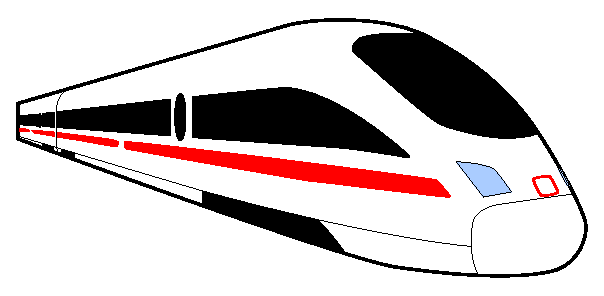
\includegraphics[scale=0.5]{img/geometria_analitica/tren.eps}}
\psline[linewidth=0.08cm,arrowsize=0.05291667cm 2.0,arrowlength=1.4,arrowinset=0.4]{->}(5.72,-0.6610938)(9.34,-1.2610937)
\usefont{T1}{ptm}{m}{n}
\rput(7.5514064,-0.69609374){$\vec{v}$}
\usefont{T1}{ptm}{m}{n}
\rput(10.043282,-1.2360938){dirección}
\psline[linewidth=0.04cm,linecolor=red,tbarsize=0.07055555cm 5.0]{|-|}(5.64,-0.9010937)(9.26,-1.5010937)
\usefont{T1}{ptm}{m}{n}
\rput(7.118906,-1.4560938){magnitud}
\end{pspicture} }
	\end{center}
\end{frame}


% ---------------------------------------------------------------------slide----
\begin{frame}
	\frametitle{Representación de un vector}
	Un segmento orientado puede ubicarse en diferentes lugares dentro de un espacio cartesiano. 
	Sin embargo, con independencia de donde esté situado, si la longitud y la dirección no varían, dicho segmento
	representará siempre el mismo vector.
	
	Esto permite representar todos los vectores con un mismo origen, el origen en sistema de coordenadas cartesianas.
	Así, un vector queda determinado por las \emph{coordenadas} de su extremo final en cualquier espacio euclideo.
	
	\begin{center}
		\scalebox{0.8}{\psset{unit=1,algebraic}
\begin{pspicture}(-4,-2.5)(4,2.5)
\psaxes[ticks=none,labels=none]{<->}(0,0)(-4,-2.5)(4,2.5)
\psline{->}(2,1.5)(4,2.5)
\rput(1.8,1.4){$A$}
\rput(4.2,2.6){$B$}
\psline{->}(-3,0.5)(-1,1.5)
\rput(-3.2,0.4){$C$}
\rput(-0.8,1.6){$D$}
\psline{->}(-1,-2)(1,-1)
\rput(-1.2,-2.1){$E$}
\rput(1.2,-0.9){$F$}
\psline[linecolor=red]{->}(0,0)(2,1)
\rput(1,0.6){$\mathbf{v}$}
\psline[linestyle=dashed, linecolor=gray](2,0)(2,1)(0,1)
\psxTick[ticksize=-3pt 0,labelsep=3pt](2){x}
\psyTick[ticksize=-3pt 0,labelsep=3pt](1){y}
\rput[l](3,0.5){${\mathbf{v}} = (x,y) = \vec{AB}=\vec{CD}=\vec{EF}$}
\end{pspicture}}
	\end{center}
\end{frame} 


% ---------------------------------------------------------------------slide----
\begin{frame}
	\frametitle{Vector a partir de dos puntos}
	Dados dos puntos $P$ y $Q$ de un espacio cartesiano, el vector con origen en $P$ y destino en $Q$ tiene coordenadas $\vec{PQ}=Q-P$.
	
	\structure{\bfseries Ejemplo} 
	Sean los puntos $P=(2,1)$  y $Q=(3,4)$ del plano real $\mathbb{R}^2$, entonces
	\[
		\vec{PQ} = Q-P = (3,4)-(2,1) = (3-2,4-1) = (1,3).
	\]
	\begin{center}
		\scalebox{0.8}{\psset{unit=1,algebraic}
\begin{pspicture}(-0.5,-0.5)(5,5)
\psaxes[labelFontSize=\scriptstyle,ticksize=-3pt 0,labelsep=2pt]{<->}(0,0)(-0.5,-0.5)(5,5)[$x$,-90][$y$,180]
\psdot(3,4)
\psline[linestyle=dashed, linecolor=gray](3,0)(3,4)(0,4)
\rput[l](3.1,4){$Q$}
\psdot(2,1)
\psline[linestyle=dashed, linecolor=gray](2,0)(2,1)(0,1)
\rput[l](2.1,1){$P$}
\psline[linecolor=red]{->}(2,1)(3,4)
\rput[r](2.4,2.5){$\vec{PQ}$}
\end{pspicture}}
	\end{center}
\end{frame} 


% ---------------------------------------------------------------------slide----
\begin{frame}
	\frametitle{Módulo de un vector}
	\begin{definicion}[Módulo de un vector]
		Dado un vector $\mathbf{v}=(v_1,\cdots,v_n)$ de $\mathbb{R}^n$, se define el \emph{módulo} de $\mathbf{v}$ como
		\[
			|\mathbf{v}| = \sqrt{v_1^2+ \cdots + v_n^2}.
		\]
	\end{definicion}
	El módulo de un vector coincide con la longitud del segmento que representa al vector.
	
	\structure{\bfseries Ejemplos} 
	Sea $\mathbf{u}=(3,4)$ un vector en $\mathbb{R}^2$, entonces
	\[
		|\mathbf{u}| = \sqrt{3^2+4^2} = \sqrt{25} = 5
	\]
	Sea $\mathbf{v}=(4,7,4)$ un vector en $\mathbb{R}^3$, entonces
	\[
		|\mathbf{v}| = \sqrt{4^2+7^2+4^2} = \sqrt{81} = 9
	\]
\end{frame} 


% ---------------------------------------------------------------------slide----
\begin{frame}
	\frametitle{Vectores unitarios}
	\begin{definicion}[Vector unitario]
		Se dice que un vector $\mathbf{v}$ de $\mathbb{R}^n$ es \emph{unitario} si su módulo es 1, es decir $|\mathbf{v}|=1$.
	\end{definicion}
	Especial atención merecen los vectores unitarios que siguen la dirección de los ejes de coordenadas, estos vectores se llaman \emph{vectores coordenados}.
	\begin{columns}
		\begin{column}{.48\textwidth}
			En $\mathbb{R}^2$ los vectores coordenados son 
			\[
				\mathbf{i}=(1,0)\mbox{ y }\mathbf{j}=(0,1)
			\]
			\begin{center}
				\scalebox{1}{\psset{unit=1,algebraic}
\begin{pspicture}(-0.5,-0.5)(2.5,2.5)
\psaxes[labelFontSize=\scriptstyle,ticksize=-3pt 0,labelsep=2pt]{<->}(0,0)(-0.5,-0.5)(2,2)[$x$,-90][$y$,180]
\psline[linecolor=red]{->}(0,0)(1,0)
\rput(0.5,0.2){$\mathbf{i}$}
\psline[linecolor=red]{->}(0,0)(0,1)
\rput(0.2,0.5){$\mathbf{j}$}
\end{pspicture}}
			\end{center}
		\end{column}
		\begin{column}{.48\textwidth}
			En $\mathbb{R}^3$ los vectores coordenados son 
			\[
				\mathbf{i}=(1,0,0)\mbox{, }\mathbf{j}=(0,1,0) \mbox{ y } \mathbf{k}=(0,0,1)
			\]
			\begin{center}
				\scalebox{1}{\psset{unit=1}
\psset{viewpoint=40 20 20 , Decran=50}
\begin{pspicture}(-0.5,-0.5)(2,2)
\axesIIID(0,0,0)(2,2,2)
\psPoint(0,0,0){O}
\psPoint(1,0,0){i}
\psPoint(0,1,0){j}
\psPoint(0,0,1){k}
\psline[linecolor=red]{->}(O)(i)
\uput[r](i){$\mathbf{i}$}
\psline[linecolor=red]{->}(O)(j)
\uput[u](j){$\mathbf{j}$}
\psline[linecolor=red]{->}(O)(k)
\uput[r](k){$\mathbf{k}$}
\end{pspicture}}
			\end{center}
		\end{column}   
	\end{columns}
\end{frame} 


% ---------------------------------------------------------------------slide----
\begin{frame}
	\frametitle{Suma de vectores}
	\begin{definicion}[Suma de vectores]
		Dados dos vectores $\mathbf{u}=(u_1,\cdots,u_n)$ y $\mathbf{v}=(v_1,\cdots,v_n)$ de $\mathbb{R}^n$, se define la
		\emph{suma} de $\mathbf{u}$ y $\mathbf{v}$ como
		\[
			\mathbf{u}+\mathbf{v} = (u_1+v_1,\ldots, u_n+v_n).
		\]
	\end{definicion}
	
	\structure{\bfseries Ejemplo} 
	Sean $\mathbf{u}=(3,1)$ y $\mathbf{v}=(2,3)$ dos vectores en $\mathbb{R}^2$, entonces
	\[
		\mathbf{u}+\mathbf{v} = (3+2,1+3) = (5,4).
	\]
	
	\begin{center}
		\scalebox{0.8}{\psset{unit=1,algebraic}
\begin{pspicture}(-0.5,-0.5)(5,4)
\psaxes[ticks=none,labels=none]{<->}(0,0)(-0.5,-0.5)(5,4)[$x$,-90][$y$,180]
\psline{->}(0,0)(3,1)
\rput(1.6,0.3){$\mathbf{u}$}
\psline[linestyle=dashed, linecolor=gray](3,0)(3,1)(0,1)
\psxTick[ticksize=-3pt 0,labelsep=3pt](3){u_1}
\psyTick[ticksize=-3pt 0,labelsep=3pt](1){u_2}
\psline{->}(0,0)(1,2)
\rput(0.4,1.2){$\mathbf{v}$}
\psline[linestyle=dashed, linecolor=gray](1,0)(1,2)(0,2)
\psxTick[ticksize=-3pt 0,labelsep=3pt](1){v_1}
\psyTick[ticksize=-3pt 0,labelsep=3pt](2){v_2}
\psline[linecolor=red]{->}(0,0)(4,3)
\rput(2,1.6){$\mathbf{u}+\mathbf{v}$}
\psline[linestyle=dashed, linecolor=gray](4,0)(4,3)(0,3)
\psxTick[ticksize=-3pt 0,labelsep=3pt](4){u_1+v_1}
\psyTick[ticksize=-3pt 0,labelsep=3pt](3){u_2+v_2}
\psline[linestyle=dashed, linecolor=gray](3,1)(4,3)
\psline[linestyle=dashed, linecolor=gray](1,2)(4,3)
\end{pspicture}}
	\end{center}
\end{frame} 


%---------------------------------------------------------------------slide----
\begin{frame}
	\frametitle{Producto de un vector por un escalar}
	\begin{definicion}[Producto de un vector por un escalar]
		Dado un vector $\mathbf{v}=(v_1,\cdots,v_n)$ de $\mathbb{R}^n$, y un escalar $a\in \mathbb{R}$, se define el
		\emph{producto} de $a$ por $\mathbf{v}$ como
		\[
			a\mathbf{v} = (av_1,\ldots, av_n).
		\]
	\end{definicion}
	\structure{\bfseries Ejemplo}
	Sean el vector $\mathbf{v}=(2,1)$ en $\mathbb{R}^2$ y el escalar $a=2$, entonces
	\[
		a\mathbf{v} = 2(2,1) = (4,2).
	\]
	
	\begin{center}
		\scalebox{0.8}{\psset{unit=1,algebraic}
\begin{pspicture}(-0.5,-0.5)(5,3)
\psaxes[ticks=none,labels=none]{<->}(0,0)(-0.5,-0.5)(5,3)[$x$,-90][$y$,180]
\psline[linecolor=red]{->}(0,0)(4,2)
\rput(2.2,1.3){$a\mathbf{v}$}
\psline[linestyle=dashed, linecolor=gray](4,0)(4,2)(0,2)
\psxTick[ticksize=-3pt 0,labelsep=3pt](4){av_1}
\psyTick[ticksize=-3pt 0,labelsep=3pt](2){av_2}
\psline{->}(0,0)(2,1)
\rput(0.9,0.7){$\mathbf{v}$}
\psline[linestyle=dashed, linecolor=gray](2,0)(2,1)(0,1)
\psxTick[ticksize=-3pt 0,labelsep=3pt](2){v_1}
\psyTick[ticksize=-3pt 0,labelsep=3pt](1){v_2}
\end{pspicture}}
	\end{center}
\end{frame}  


%---------------------------------------------------------------------slide----
\begin{frame}
	\frametitle{Expresión de un vector como combinación lineal de los vectores coordenados}
	La suma de vectores y el producto de un vector por un escalar permite expresar cualquier vector como una combinación lineal de los vectores coordenados.
	
	En el caso del espacio real $\mathbb{R}^3$, cualquier vector $\mathbf{v}=(v_1,v_2,v_3)$ puede expresarse como   
	\[
		\mathbf{v}=(v_1,v_2,v_3) = v_1\mathbf{i}+v_2\mathbf{j}+v_3\mathbf{k}.
	\]
	
	\begin{center}
		\scalebox{0.8}{\psset{unit=1}
\psset{viewpoint=40 20 20,Decran=50}
\begin{pspicture}(0,0)(3,3)
\axesIIID(0,0,0)(3,3,3)
\psPoint(0,0,0){O}
\psPoint(1,0,0){i}
\psPoint(0,1,0){j}
\psPoint(0,0,1){k}
\psPoint(1,2,3){v}
\psline[linecolor=red]{->}(O)(i)
\uput[r](i){$\mathbf{i}$}
\psline[linecolor=red]{->}(O)(j)
\uput[u](j){$\mathbf{j}$}
\psline[linecolor=red]{->}(O)(k)
\uput[r](k){$\mathbf{k}$}
\psline[linecolor=blue]{->}(O)(v)
\psPoint(1,1.4,2){v2}
\uput[r](v2){$\mathbf{v}$}
\psPoint(1,2,0){xy}
\psPoint(0,2,0){j2}
\psline[linestyle=dashed, linecolor=gray](i)(xy)(j2)
\psline[linestyle=dashed, linecolor=gray](xy)(v)
\psPoint(1,0,3){xz}
\psPoint(0,0,3){k3}
\psline[linestyle=dashed, linecolor=gray](i)(xz)(k3)
\psline[linestyle=dashed, linecolor=gray](xz)(v)
\psPoint(0,2,3){yz}
\psline[linestyle=dashed, linecolor=gray](j2)(yz)(k3)
\psline[linestyle=dashed, linecolor=gray](yz)(v)
\psPoint(1,1,0){a}
\uput[d](a){$v_2$}
\psPoint(0.8,2,0){b}
\uput[r](b){$v_1$}
\psPoint(0,2,1.5){c}
\uput[r](c){$v_3$}
\end{pspicture}}
	\end{center}
\end{frame} 


%---------------------------------------------------------------------slide----
\begin{frame}
	\frametitle{Producto escalar}
	\begin{definicion}[Producto escalar]
		Dados dos vectores $\mathbf{u}=(u_1,\cdots,u_n)$ y $\mathbf{v}=(v_1,\cdots,v_n)$ de $\mathbb{R}^n$, se define el
		\emph{producto escalar} de $\mathbf{u}$ y $\mathbf{v}$ como
		\[
			\mathbf{u}\cdot \mathbf{v} = u_1v_1 + \cdots + u_nv_n.
		\]
	\end{definicion}
	\structure{\bfseries Ejemplo} 
	Sean $\mathbf{u}=(3,1)$ y $\mathbf{v}=(2,3)$ dos vectores en $\mathbb{R}^2$, entonces
	\[
		\mathbf{u}\cdot\mathbf{v} = 3\cdot 2 +1\cdot 3 = 9.
	\]
	
	Se cumple que
	\[
		\mathbf{u}\cdot\mathbf{v} =  |\mathbf{u}||\mathbf{v}|\cos\alpha
	\]
	donde $\alpha$ es el ángulo que forman los vectores.
\end{frame} 


%---------------------------------------------------------------------slide----
\begin{frame}
	\frametitle{Vectores paralelos}
	\begin{definicion}[Vectores paralelos]
		Dos vectores $\mathbf{u}$ y $\mathbf{v}$ son \emph{paralelos} si existe un valor $a\in\mathbb{R}$ tal que
		\[
			\mathbf{u} = a\mathbf{v}.
		\]
	\end{definicion}
	
	\structure{\bfseries Ejemplos} 
	Los vectores $\mathbf{u}=(-4,2)$ y $\mathbf{v}=(2,-1)$ en $\mathbb{R}^2$ son paralelos, ya que
	\[
		\mathbf{v}= (-4,2) = -2(2,-1) = -2\mathbf{v}.
	\]
	
\end{frame} 


%---------------------------------------------------------------------slide----
\begin{frame}
	\frametitle{Vectores ortogonales y ortonormales}
	\begin{definicion}[Vectores ortogonales y ortonormales]
		Dos vectores $\mathbf{u}$ y $\mathbf{v}$ son \emph{ortogonales} si su producto escalar es nulo
		\[
			\mathbf{u}\cdot \mathbf{v} = 0.
		\]
		Si además el módulo de ambos vectores es la unidad $|\mathbf{u}|=|\mathbf{v}|=1$, entonces se dice que son \emph{ortonormales}.
	\end{definicion}
	
	Los vectores ortogonales son perpendiculares entre sí, es decir, forman un ángulo de $90^\circ$.
	
	\structure{\bfseries Ejemplos} 
	Los vectores $\mathbf{u}=(2,1)$ y $\mathbf{v}=(-2,4)$ en $\mathbb{R}^2$ son ortogonales, ya que
	\[
		\mathbf{u}\mathbf{v} = 2\cdot -2 +1\cdot 4 = 0,
	\]
	pero no son ortonormales ya que $|\mathbf{u}| = \sqrt{2^2+1^2} \neq 1$ y  $|\mathbf{v}| = \sqrt{-2^2+4^2} \neq 1$.
	
	Los vectores $\mathbf{i}=(1,0)$ y $\mathbf{j}=(0,1)$ en $\mathbb{R}^2$ son ortonormales, ya que
	\[
		\mathbf{i}\mathbf{j} = 1\cdot 0 +0\cdot 1 = 0, \quad |\mathbf{i}| = \sqrt{1^2+0^2} = 1,  \quad |\mathbf j| = \sqrt{0^2+1^2} = 1.
	\]
\end{frame}  



\subsection{Rectas}
%---------------------------------------------------------------------slide----
\begin{frame}
	\frametitle{Ecuación vectorial de la recta}
	\begin{definicion}[Ecuación vectorial de la recta]
		Sea $l$ una recta del espacio $\mathbb{R}^n$ y sean $P=(p_1,\ldots,p_n)$ un punto cualquiera de la recta y
		$\mathbf{v}=(v_1,\ldots,v_n)$ un vector cualquiera con la misma dirección que la recta.
		La ecuación
		\[
			l: X= P + t\mathbf{v} = (p_1,\ldots,p_n)+t(v_1,\ldots,v_n) = (p_1+tv_1,\ldots,p_n+tv_n).
		\]
		parametriza a $l$ en función de $t\in \mathbb{R}$, y se conoce como \emph{ecuación vectorial de la recta}.
	\end{definicion}
	\begin{columns}
		\begin{column}{.48\textwidth}
			\structure{\bfseries Ejemplo} 
			Considerese la recta del espacio real $\mathbb{R}^3$ que aparece en la gráfica. Un punto de la recta es $P=(1,1,2)$ y un vector director es $\mathbf{v}=(-1,2,2)$, luego su ecuación vectorial es
			\begin{align*}
				l & : X= P + t\mathbf{v} = (1,1,2)+t(-1,2,1) = \\
				  & = (1-t,1+2t,2+t)\quad t\in\mathbb{R}.      
			\end{align*}
		\end{column}
		\begin{column}{.48\textwidth}
			\begin{center}
				\scalebox{0.8}{\psset{unit=1}
\psset{viewpoint=40 20 20,Decran=40}
\begin{pspicture}(0,0)(2,2)
\axesIIID(0,0,0)(3,3,3)
\psPoint(0,0,0){O}
\psPoint(1,1,2){P}
\psPoint(0,3,3){v}
\psSolid[object=line,args=2 -1 1 -1 5 4]
\psSolid[object=point,args=1 1 2]
\psline[linecolor=red]{->}(P)(v)
\uput[d](P){$P$}
\psPoint(0.5,2,2.5){v2}
\uput[u](v2){$\mathbf{v}$}
\psPoint(-1,5,4){l}
\uput[r](l){$l$}
\end{pspicture}}
			\end{center}
		\end{column}
	\end{columns}
\end{frame} 


%---------------------------------------------------------------------slide----
\begin{frame}
	\frametitle{Ecuaciones paramétricas y cartesianas de la recta}
	De la ecuación vectorial de una recta $l: X=P + t\mathbf{v}=(p_1+tv_1,\ldots,p_n+tv_n)$ se obtienen facilmente las coordenadas de los puntos que forman parte de la recta mediante $n$ ecuaciones paramétricas:
	\[
		x_1(t)=p_1+tv_1, \ldots, x_n(t)=p_n+tv_n
	\]
	donde, si $\mathbf{v}$ es un vector cuyas coordenadas son no nulas ($v_i\neq 0$ $\forall i$), se puede despejar el parámetro $t$ en cada una de ellas e igualarlas,
	\[
		\frac{x_1-p_1}{v_1}=\cdots = \frac{x_n-p_n}{v_n}
	\] 
	
	\structure{\bfseries Ejemplo} 
	Dada la ecuación vectorial de la recta $l: X=(1,1,2)+t(-1,2,1) =(1-t,1+2t,2+t)$ en el espacio real $\mathbb{R^3}$, sus
	ecuaciones paramétricas son
	\[
		x(t) = 1-t, \quad y(t)=1+2t, \quad z(t)=2+t,
	\]
	y sus ecuaciones cartesianas son
	\[
		\frac{x-1}{-1}=\frac{y-1}{2}=\frac{z-2}{1}
	\]
\end{frame} 


%---------------------------------------------------------------------slide----
\begin{frame}
	\frametitle{Ecuación punto-pendiente de una recta en el plano}
	En el caso particular del plano cartesiano $\mathbb{R^2}$, si se tiene una recta con ecuación vectorial $l: X=P+t\mathbf{v}=(x_0,y_0)+t(a,b)
	= (x_0+ta,y_0+tb)$, sus ecuaciones paramétricas son
	\[
		x(t)=x_0+ta,\quad y(t)=y_0+tb
	\]
	y sus ecuación cartesiana es
	\[
		\frac{x-x_0}{a} = \frac{y-y_0}{b}.
	\]  
	A partir de aquí, pasando $b$ multiplicando al otro lado de la ecuación, se obtiene 
	\[
		y-y_0 = \frac{b}{a}(x-x_0) \mbox{ o bien } y-y_0+m(x-x_0),
	\]
	llamando $m=b/a$. Esta ecuación se conoce como ecuación en la forma \emph{punto-pendiente}.
	 
\end{frame} 


%---------------------------------------------------------------------slide----
\begin{frame}
	\frametitle{Pendiente de una recta en el plano}
	\begin{definicion}[Pendiente de una recta]
		Dada una recta $l: X=P+t\mathbf{v}$ en el plano real $\mathbb{R}^2$, con vector director $\mathbf{v}=(a,b)$, se define la pendiente de $l$ como $b/a$.
	\end{definicion}
	
	Recordar que dados dos puntos $Q=(x_1,y_1)$ y $Q=(x_2,y_2)$ de la recta $l$, se puede tomar como vector director el vector que los une, que tiene coordenadas $\vec{PQ}=Q-P=(x_2-x_1,y_2-y_1)$, de manera que la pendiente de $l$ será 
	$\dfrac{y_2-y_1}{x_2-x_1}$, es decir, el cociente entre lo que cambia la coordenada $y$ y lo que cambia la coordenada $x$.
	
	\begin{center}
		\scalebox{0.7}{\psset{unit=1,algebraic}
\begin{pspicture*}(-0.5,-0.5)(5.2,4.2)
\psaxes[ticks=none,labels=none]{<->}(0,0)(-0.5,-0.5)(5,4)[$x$,-90][$y$,180]
\psdot(4,3)
\psline[linestyle=dashed, linecolor=gray](4,0)(4,3)(0,3)
\rput[l](4.1,2.9){$Q$}
\psdot(1,1)
\psline[linestyle=dashed, linecolor=gray](1,0)(1,1)(0,1)
\rput[u](1,1.2){$P$}
\psline(-2,-1)(7,5)
\psline[linecolor=red]{->}(1,1)(4,3)
\rput[r](2.5,2.5){$\vec{PQ}$}
\psline[linestyle=dashed, linecolor=orange](1,1)(4,1)(4,3)
\psxTick[ticksize=-3pt 0,labelsep=3pt](1){x_1}
\psxTick[ticksize=-3pt 0,labelsep=3pt](4){x_2}
\psyTick[ticksize=-3pt 0,labelsep=3pt](1){y_1}
\psyTick[ticksize=-3pt 0,labelsep=3pt](3){y_2}
\rput[u](2.5,0.8){$x_2-x_1$}
\rput[l](4.1,2){$y_2-y_1$}
\rput[l](4.1,2){$y_2-y_1$}
\rput[l](4.7,3.7){$l$}
\end{pspicture*}}
	\end{center}
\end{frame} 



\subsection{Planos}
%---------------------------------------------------------------------slide----
\begin{frame}
	\frametitle{Ecuación del plano en el espacio real}
	Para llegar a la ecuación de un plano en el espacio real $\mathbb{R}^3$ se puede partir de un punto del plano $P=(x_0,y_0,z_0)$ y de un vector perpendicular al plano $\mathbf{v}=(a,b,c)$. 
	Entonces, para cualquier punto del plano $Q=(x,y,z)$ se cumple que el vector $\vec{PQ} = (x-x_0,y-y_0,z-z_0)$ es ortogonal a $\mathbf{v}$, por lo que su producto escalar se anulará
	\[
		\vec{PQ}\cdot\mathbf{v} = (x-x_0,y-y_0,z-z_0)(a,b,c) = a(x-x_0)+b(y-y_0)+c(z-z_0) = 0.
	\]
	
	\begin{center}
		\scalebox{0.8}{\psset{unit=1,viewpoint=40 10 5,Decran=40}
\begin{pspicture}(-3,-3)(5,4)
\psSolid[object=plan, definition=normalpoint, args={1 1 1 [1 2 2]}, fillcolor=cyan, base=-2 2 -2 2]
\psSolid[object=point,args=1 1 1]
\psPoint(1,1,1){P}
\uput[l](P){$P$}
\psPoint(1,2,0){Q}
\uput[d](Q){$Q$}
\psline{->}(P)(Q)
\psPoint(1,2,2){v}
\uput[r](v){$\mathbf{v}$}
\psline[linecolor=red]{->}(P)(v)
\axesIIID(0,0,0)(5,4,3.5)
\end{pspicture}}
	\end{center}
\end{frame} 




\section{Funciones reales de variable real}

%---------------------------------------------------------------------slide----
\mode<presentation>{
	\begin{frame}
		\frametitle{Funciones reales de variable real}
		\setlength{\parskip}{0.3em}
		\tableofcontents[sectionstyle=show/hide,hideothersubsections]
	\end{frame}
}

\subsection{El concepto de función}

%---------------------------------------------------------------------slide----
\begin{frame}
	\frametitle{¿Qué es una función?}
	\begin{definicion}[Función de una variable]
		Una \emph{función} $f$ de un conjunto $A$ en otro $B$ es una \emph{relación} que asocia cada elemento $a\in A$, con un \emph{único} elemento de $B$ que se denota $f(a)$, y se llama \emph{imagen} de $a$ mediante $f$.
		\begin{align*}
			f:\, & A\longrightarrow B    \\
			     & a\longrightarrow f(a) 
		\end{align*}
	\end{definicion}
	
	\begin{center}
		\scalebox{1}{\psset{unit=0.5}
\begin{pspicture*}(0,0)(10,4)
\psellipse(2,2)(1.5,2)
\psellipse(8,2)(1.5,2)
\rput(2.2,3){3}
\rput(1.8,2){4}
\rput(2.1,1){5}
\rput(7.6,1.7){\pspolygon*(0,0)(0.5,0.7)(1,0)}
\rput(7.5,2.7){\psframe*(0.6,0.6)}
\rput(7.6,0.7){\pspolygon*(0.2,0)(0,0.4)(0.5,0.6)(1,0.4)(0.8,0)}
\psline[arrows=->](2.6,3)(7.3,2)
\psline[arrows=->](2.6,2)(7.3,3)
\psline[arrows=->](2.6,1)(7.3,1)
\end{pspicture*}}
	\end{center}
	Cuando el conjunto inicial y final es el de los números reales $\mathbb{R}$, entonces se dice que 
	$f:\mathbb{R}\rightarrow \mathbb{R}$ es una \emph{función real de variable real}.
\end{frame}


%---------------------------------------------------------------------slide----
\begin{frame}
	\frametitle{Formas de representar una función}
	\begin{columns}
		\begin{column}{.48\textwidth}
			\textbf{Por extensión}
			\begin{block}{Representación en tabla}
				\[
					\begin{array}{|c|c|c|c|c|c|c|}
						\hline
						x & -2 & -1 & 0 & 1 & 2 & \cdots \\
						\hline
						y & 4  & 1  & 0 & 1 & 4 & \cdots \\
						\hline
					\end{array}
				\]
			\end{block}
			\begin{block}{Representación gráfica}
				\begin{center}
					\scalebox{0.7}{\psset{unit=1,algebraic}
\begin{pspicture}(-2,-1)(2,4.5)
\psaxes[labelFontSize=\scriptstyle,ticksize=-3pt 0,labelsep=2pt]{<->}(0,0)(-2.5,-1)(2.5,4.5)
\psplot[linecolor=blue]{-2}{2}{x^2}
\psline[linecolor=red,linestyle=dotted](1.5,-0.1)(1.5,2.25)(-0.1,2.25)
\psxTick[ticksize=-3pt 0,labelsep=3pt](1.5){\color{red}x}
\psyTick[ticksize=-3pt 0,labelsep=3pt](2.25){\color{red}y}
\end{pspicture}}
				\end{center}
			\end{block}
		\end{column}
		\begin{column}{.48\textwidth}
			\textbf{Por Intensión}
			\begin{block}{Representación algebraica explícita}
				\[y=x^2\]
			\end{block}
			\begin{block}{Representación algebraica implícita}
				\[y-x^2=0\]
			\end{block}
			\begin{block}{Representación algebraica paramétrica}
				\[  
					\begin{cases}
						y=t^2 \\
						x=t   
					\end{cases}
				\]
			\end{block}
		\end{column}   
	\end{columns}
\end{frame} 


%---------------------------------------------------------------------slide----
\begin{frame}
	\frametitle{La función Identidad}
	\begin{definicion}[Función Identidad]
		Se llama \emph{función identidad}, a toda función $Id: A\rightarrow A$ que asocia cada elemento de $A$ con sigo mismo, es decir, 
		\[Id(x)=x.\]
	\end{definicion}
	\begin{center}
		\scalebox{1}{\psset{unit=0.8,algebraic}
\begin{pspicture*}(-3,-3)(3,3)
\psaxes[labelFontSize=\scriptstyle,ticksize=-3pt 0,labelsep=2pt]{<->}(0,0)(-3,-3)(3,3)
\psplot[linecolor=blue]{-2}{2}{x}
\rput[l](1,2.5){$f(x)=x$}
\end{pspicture*}}
	\end{center}
\end{frame} 



\subsection{Dominio e imagen de una función}
%---------------------------------------------------------------------slide----
\begin{frame}
	\frametitle{Dominio de una función}
	\begin{definicion}[Dominio de una función]
		El \emph{dominio} de una función $f$ es el conjunto de valores para los que la función está definida
		\[
			Dom(f)=\{x\in \mathbb{R}: f(x)\in \mathbb{R}\}
		\]
	\end{definicion}
	\structure{\bfseries Ejemplo}
	\begin{center}
		\scalebox{1}{\psset{unit=0.8,algebraic}
\begin{pspicture*}(-5,-0.5)(5,4)
\psaxes[labelFontSize=\scriptstyle,ticksize=-3pt 0,labelsep=2pt]{<->}(0,0)(-3.3,-0.5)(3.3,4)
\psplot[linecolor=blue]{-3}{-1.00001}{1/sqrt(x^2-1)}
\psplot[linecolor=blue]{1.00001}{3}{1/sqrt(x^2-1)}
\rput[l](1.3,2){$f(x)=\dfrac{1}{\sqrt{x^2-1}}$}
\uncover<2->{
\psline[linecolor=red,linewidth=1pt,tbarsize=7pt 0]{<-)}(-3.3,0)(-1,0)
\psline[linecolor=red,linewidth=1pt,tbarsize=7pt 0]{(->}(1,0)(3.3,0)
}
\end{pspicture*}}\\
		$\mbox{Dom}(f)=(-\infty,-1)\cup(1,\infty)$
	\end{center}
\end{frame} 


%---------------------------------------------------------------------slide----
\begin{frame}
	\frametitle{Imagen de una función}
	\begin{definicion}[Imagen de una función]
		La \emph{imagen} de una función $f$ es el conjunto de valores que la función puede tomar
		\[
			Img(f)=\{y\in \mathbb{R}: y=f(x) \mbox{ para algún } x\in\mathbb{R}\}
		\]
	\end{definicion}
	\structure{\bfseries Ejemplo}
	\begin{center}
		\scalebox{1}{\psset{unit=0.7,algebraic}
\begin{pspicture*}(-5,-3)(5,3)
\psaxes[labelFontSize=\scriptstyle,ticksize=-3pt 0,labelsep=2pt]{<->}(0,0)(-3,-3)(3,3)
\psplot[linecolor=blue]{-2}{2}{x^2-2}
\normalsize
\rput[l](1,2.5){$f(x)=x^2-2$}
\uncover<2->{
\psline[linecolor=red,linewidth=1pt,tbarsize=7pt 0,arrows=[->](0,-2)(0,3)
}
\end{pspicture*}}\\
		$\mbox{Img}(f)=[-2,\infty)$
		\end{center}
	\end{frame} 
	
	
	
	\subsection{Composición e inversa de una función}
	%---------------------------------------------------------------------slide----
	\begin{frame}
		\frametitle{Composición de funciones}
		\begin{definicion}[Composición de funciones]
			Dadas dos funciones $g:A\rightarrow B$ y $f:B\rightarrow C$, se define la \emph{función compuesta} $f\circ g$, (leído $g$ compuesto con $f$) como la función  
			\begin{align*}
				f\circ g:\, & A\longrightarrow C       \\
				            & x\longrightarrow f(g(x)) 
			\end{align*}
		\end{definicion}
		Para calcular la función compuesta $f\circ g(x)$, primero se aplica $g$ sobre $x$ y luego, se aplica $f$ sobre $g(x)$:
		\[
			x\stackrel{g}{\longrightarrow}g(x)\stackrel{f}{\longrightarrow}f(g(x))
		\]
		\structure{\textbf{Ejemplo}} Si $g(x)=\sqrt x$ y $f(x)=\sen x$, entonces 
		\[
			f\circ g(x)=f(g(x))=f(\sqrt x)=\sen \sqrt x.
		\]
		\begin{center}
			\emph{¿Cuál es su dominio?}
		\end{center}
	\end{frame} 
	
	
	%---------------------------------------------------------------------slide----
	\begin{frame}
		\frametitle{Inversa de una función}
		\begin{definicion}[Función inversa]
			Se llama \emph{función inversa} de $f:A\rightarrow B$ a la función $f^{-1}:B\rightarrow A$ (cuando exista) que cumple
			\[
				f\circ f^{-1}=f^{-1}\circ f=Id(x)
			\]
		\end{definicion}
		
		La función inversa de $f$ deshace o revierte el efecto de $f$. 
		Es decir, si $f:A\rightarrow B$ asocia un elemento $x\in A$ con otro $y\in B$,
		entonces $f^{-1}$ asocia el elemento $y$ con el $x$: 
		\begin{center}
			\scalebox{1}{\begin{pspicture*}(-5,-0.7)(5,0.7)
\rput[l](1,0){$y$}
\rput[r](-1,0){$x$}
\pscurve{->}(-0.8,0.1)(0,0.2)(0.8,0.1)
\rput[b](0,0.3){$f$}
\pscurve{<-}(-0.8,-0.1)(0,-0.2)(0.8,-0.1)
\rput[t](0,-0.3){$f^{-1}$}
\end{pspicture*}}
		\end{center}
		
		\structure{\textbf{Ejemplo}}
		\begin{itemize}
			\item[--] La inversa de $f(x)=x^3$ es la función $f^{-1}(x)=\sqrt[3]{x}.$ 
			\item[--] La función $x^2$ no tiene inversa. ¿Por qué?
		\end{itemize}
	\end{frame} 
	
	
	
	\subsection{Crecimiento de una función}
	%---------------------------------------------------------------------slide----
	\begin{frame}
		\frametitle{Crecimiento de una función}
		\begin{definicion}[Función creciente y decreciente]
			Se dice que una función $f$ es \emph{creciente} en un intervalo $I$, si para todo $x_1,x_2\in I$, con $x_1<x_2$, se
			cumple $f(x_1)\leq f(x_2)$.
			
			Se dice que una función $f$ es \emph{decreciente} en un intervalo $I$, si para todo $x_1,x_2\in I$, con $x_1<x_2$, se
			cumple $f(x_1)\geq f(x_2)$.
		\end{definicion}
		
		\begin{columns}
			\begin{column}{0.4\textwidth}
				\begin{center}
					\scalebox{1}{\psset{unit=1.2,algebraic}
\begin{pspicture*}(-1,-0.5)(3,2.5)
\psaxes[ticks=none,labels=none]{<->}(0,0)(-0.5,-0.5)(2.5,2.5)
\psplot[linecolor=blue]{0.5}{1.7}{x^1.5}
\psline[linecolor=red,linestyle=dashed](1,0)(1,1)(0,1)
\psline[linecolor=red,linestyle=dashed](1.5,0)(1.5,1.8371)(0,1.8371)
\psxTick[ticksize=-3pt 0,labelsep=3pt](1){x_1}
\psxTick[ticksize=0,labelsep=3pt](1.25){<}
\psxTick[ticksize=-3pt 0,labelsep=3pt](1.5){x_2}
\psyTick[ticksize=-3pt 0,labelsep=3pt](1){f(x_1)}
\psyTick[ticksize=0,labelsep=10pt](1.415){\rotateleft{\leq}}
\psyTick[ticksize=-3pt 0,labelsep=3pt](1.8371){f(x_2)}
\end{pspicture*}}\\
					\color{red}Función creciente
				\end{center}
			\end{column}
			\begin{column}{0.4\textwidth}
				\begin{center}
					\scalebox{1}{\psset{unit=1.2,algebraic}
\begin{pspicture*}(-1,-0.5)(3,2.5)
\psaxes[ticks=none,labels=none]{<->}(0,0)(-0.5,-0.5)(2.5,2.5)
\psplot[linecolor=blue]{0.5}{1.7}{2.5-x^1.5}
\psline[linecolor=red,linestyle=dashed](0.8,0)(0.8,1.7845)(0,1.7845)
\psline[linecolor=red,linestyle=dashed](1.3,0)(1.3,1.0178)(0,1.0178)
\psxTick[ticksize=-3pt 0,labelsep=3pt](0.8){x_1}
\psxTick[ticksize=0,labelsep=3pt](1.05){<}
\psxTick[ticksize=-3pt 0,labelsep=3pt](1.3){x_2}
\psyTick[ticksize=-3pt 0,labelsep=3pt](1.7845){f(x_1)}
\psyTick[ticksize=0,labelsep=10pt](1.415){\rotateleft{\leq}}
\psyTick[ticksize=-3pt 0,labelsep=3pt](1.0178){f(x_2)}
\end{pspicture*}}\\
					\color{red}Función decreciente
				\end{center}
			\end{column}
		\end{columns}
	\end{frame} 
	
	
	
	\subsection{Extremos de una función}
	%---------------------------------------------------------------------slide----
	\begin{frame}
		\frametitle{Extremos de una función}
		\begin{definicion}[Máximo y mínimo relativo]
			Se dice que una función $f$ tiene un \emph{máximo relativo} en $x_0$, si existe un $\delta>0$ tal que para todo $x\in
			(x_0-\delta,x_0+\delta)$ se cumple $f(x_0)\geq f(x)$.
			
			Se dice que una función $f$ tiene un \emph{mínimo relativo} en $x_0$, si existe un $\delta>0$ tal que para todo $x\in
			(x_0-\delta,x_0+\delta)$ se cumple $f(x_0)\leq f(x)$.
		\end{definicion}
		
		\begin{columns}
			\begin{column}{0.4\textwidth}
				\begin{center}
					\scalebox{1}{\psset{unit=1,algebraic}
\begin{pspicture*}(-1,-0.5)(3.5,2.5)
\psaxes[ticks=none,labels=none]{<->}(0,0)(-0.5,-0.5)(3.5,2.5)
\psplot[linecolor=blue]{0.5}{3.1}{2-(x-1.8)^2}
\psline[linecolor=red,linestyle=dashed](1.8,0)(1.8,2)(0,2)
\psline[linecolor=red,linestyle=dashed](1,0)(1,1.36)(0,1.36)
\footnotesize
\psxTick[ticksize=-3pt 0,labelsep=3pt](1.8){x_0}
\psxTick[ticksize=-3pt 0,labelsep=3pt](1){x}
\psyTick[ticksize=-3pt 0,labelsep=3pt](2){f(x_0)}
\psyTick[ticksize=-3pt 0,labelsep=3pt](1.36){f(x)}
\psyTick[ticksize=0,labelsep=10pt](1.72){\rotateleft{\leq}}
\rput(0.5,0){$($}
\psxTick[ticksize=-3pt 0,labelsep=3pt](0.5){x_0-\delta}
\rput(3.1,0){$)$}
\psxTick[ticksize=-3pt 0,labelsep=3pt](3.1){x_0+\delta}
\psdot[linecolor=green](1.8,2)
\end{pspicture*}}\\
					\color{red}Máximo
				\end{center}
			\end{column}
			\begin{column}{0.4\textwidth}
				\begin{center}
					\scalebox{1}{\psset{unit=1,algebraic}
\begin{pspicture*}(-1,-0.5)(3.5,2.5)
\psaxes[ticks=none,labels=none]{<->}(0,0)(-0.5,-0.5)(3.5,2.5)
\psplot[linecolor=blue]{0.5}{3.1}{(x-1.8)^2+0.5}
\psline[linecolor=red,linestyle=dashed](1.8,0)(1.8,0.5)(0,0.5)
\psline[linecolor=red,linestyle=dashed](1,0)(1,1.14)(0,1.14)
\footnotesize
\psxTick[ticksize=-3pt 0,labelsep=3pt](1.8){x_0}
\psxTick[ticksize=-3pt 0,labelsep=3pt](1){x}
\psyTick[ticksize=-3pt 0,labelsep=3pt](0.5){f(x_0)}
\psyTick[ticksize=-3pt 0,labelsep=3pt](1.14){f(x)}
\psyTick[ticksize=0,labelsep=8pt](0.8){\rotateleft{\leq}}
\rput(0.5,0){$($}
\psxTick[ticksize=-3pt 0,labelsep=3pt](0.5){x_0-\delta}
\rput(3.1,0){$)$}
\psxTick[ticksize=-3pt 0,labelsep=3pt](3.1){x_0+\delta}
\psdot[linecolor=green](1.8,0.5)
\end{pspicture*}}\\
					\color{red}Mínimo
				\end{center}
			\end{column}
		\end{columns}
	\end{frame} 
	
	
	\subsection{Concavidad de una función}
	
	%---------------------------------------------------------------------slide----
	\begin{frame}
		\frametitle{Concavidad de una función}
		\begin{definicion}[Función cóncava y convexa]
			Se dice que una función $f$ es \emph{cóncava} en un intervalo $I$, si para todo $x_1,x_2\in I$, con $x_1<x_2$, se cumple
			que el segmento que une los puntos $(x_1,f(x_1))$ y $(x_2,f(x_2))$ queda por encima de la gráfica de $f$.
			
			Se dice que una función $f$ es \emph{convexa} en un intervalo $I$, si para todo $x_1,x_2\in I$, con $x_1<x_2$, se cumple
			que el segmento que une los puntos $(x_1,f(x_1))$ y $(x_2,f(x_2))$ queda por debajo de la gráfica de $f$.
			
			Al punto donde cambia la concavidad de una función se le llama \emph{punto de inflexión}.
		\end{definicion}
		
		\begin{columns}
			\begin{column}{0.4\textwidth}
				\begin{center}
					\scalebox{1}{\psset{unit=1,algebraic}
\begin{pspicture*}(-1,-0.5)(3.5,2.5)
\psaxes[ticks=none,labels=none]{<->}(0,0)(-0.5,-0.5)(3.5,2.5)
\psplot[linecolor=blue]{0.5}{3.1}{(x-1.8)^2+0.5}
\psline[linecolor=red,linestyle=dashed](0.9,0)(0.9,1.31)(0,1.31)
\psline[linecolor=red,linestyle=dashed](2.9,0)(2.9,1.71)(0,1.71)
\psline[linecolor=green]{<->}(0.9,1.31)(2.9,1.71)
\psxTick[ticksize=-3pt 0,labelsep=3pt](0.9){x_1}
\psxTick[ticksize=-3pt 0,labelsep=3pt](2.9){x_2}
\psyTick[ticksize=-3pt 0,labelsep=3pt](1.31){f(x_1)}
\psyTick[ticksize=-3pt 0,labelsep=3pt](1.71){f(x_2)}
\end{pspicture*}}\\
					\color{red}Función cóncava
				\end{center}
			\end{column}
			\begin{column}{0.4\textwidth}
				\begin{center}
					\scalebox{1}{\psset{unit=1,algebraic}
\begin{pspicture*}(-1,-0.5)(3.5,2.5)
\psaxes[ticks=none,labels=none]{<->}(0,0)(-0.5,-0.5)(3.5,2.5)
\psplot[linecolor=blue]{0.5}{3.1}{2-(x-1.8)^2}
\psline[linecolor=red,linestyle=dashed](0.9,0)(0.9,1.19)(0,1.19)
\psline[linecolor=red,linestyle=dashed](2.9,0)(2.9,0.79)(0,0.79)
\psline[linecolor=green]{<->}(0.9,1.19)(2.9,0.79)
\psxTick[ticksize=-3pt 0,labelsep=3pt](0.9){x_1}
\psxTick[ticksize=-3pt 0,labelsep=3pt](2.9){x_2}
\psyTick[ticksize=-3pt 0,labelsep=3pt](1.19){f(x_1)}
\psyTick[ticksize=-3pt 0,labelsep=3pt](0.79){f(x_2)}
\end{pspicture*}}\\
					\color{red}Función convexa
				\end{center}
			\end{column}
		\end{columns}
	\end{frame} 
	
	
	
	\subsection{Funciones periódicas}
	%---------------------------------------------------------------------slide----
	\begin{frame}
		\frametitle{Funciones periódicas}
		\begin{definicion}[Función periódica y periodo]
			Se dice que una función $f$ es \emph{periódica} si existe un valor $h>0$ tal que
			\[f(x+h)=f(x)\]
			para todo $x\in \textrm{Dom}(f)$.
			
			Al menor valor de $h$ que verifica la igualdad anterior se le llama \emph{periodo} de $f$, y a la mitad de la diferencia entre el
			máximo y el mínimo de la función se le llama \emph{amplitud} de $f$.
		\end{definicion}
		
		\begin{center}
			\scalebox{0.8}{\psset{unit=1.5,algebraic}
\begin{pspicture*}(-4,-1.5)(3.5,1.5)
\psaxes[ticks=none,labels=none]{<->}(-1.9634,0)(-2.1,-1.3)(2.1,1.3)
\psplot[linecolor=blue,plotpoints=100]{-1.9634}{2}{cos(4*x)}
\psline[linecolor=red]{|-|}(-1.57075,1)(0,1)
\rput[b](-0.78,1.1){\color{red}Periodo}
\psline[linecolor=red]{|-|}(0,0)(0,1)
\rput[r](-0.1,0.5){\rotateleft{\color{red}Amplitud}}
\end{pspicture*}}
		\end{center}
	\end{frame} 
	
	
	
	\subsection{Funciones polinómicas}
	%---------------------------------------------------------------------slide----
	\begin{frame}
		\frametitle{Funciones polinómicas}
		\begin{definicion}[Función polinómica]
			Una \emph{función polinómica} es una función de la forma
			\[
				f(x)=a_0+a_1x+a_2x^2+\cdots+a_nx^n,
			\]
			donde $n$ es un entero no negativo que se llama \emph{grado del polinomio}, y $a_0,\ldots,a_n$ son constantes reales
			($a_n\neq 0$) que se llaman \emph{coeficientes del polinomio}.
		\end{definicion}
		\begin{center}
			\scalebox{1}{\psset{unit=0.6,algebraic}
\begin{pspicture*}(-8,-2)(8,4)
\psaxes[labelFontSize=\scriptstyle,ticksize=-3pt 0,labelsep=2pt]{<->}(0,0)(-3,-2)(3,4)
\psplot[linecolor=blue]{-3}{3}{2*x^2+x-1}
\psplot[linecolor=red]{-3}{3}{x^3-x^2-2*x+2}
\footnotesize
\rput[l](-5.5,2){$f(x)=2x^2+x-1$}
\rput[l](-6.5,-1.5){$g(x)=x^3-x^2-2x+2$}
\end{pspicture*}}
		\end{center}
	\end{frame} 
	
	%---------------------------------------------------------------------slide----
	\begin{frame}
		\frametitle{Propiedades de las funciones polinómicas}
		\begin{itemize}
			\item Su dominio es $\mathbb{R}$.
			\item Si el grado es impar, su imagen es $\mathbb{R}$.
			\item La función identidad $Id(x)=x$ es un polinomio de grado 1.
			\item Las funciones constantes $f(x)=c$ son polinomios de grado 0.
			\item Un polinomio de grado $n$ tiene a lo sumo $n$ raíces (puntos donde $f(x)=0$). 
		\end{itemize}
	\end{frame} 
	
	
	
	\subsection{Funciones racionales}
	%---------------------------------------------------------------------slide----
	\begin{frame}
		\frametitle{Funciones racionales}
		\begin{definicion}[Función racional]
			Una \emph{función racional} es una función de la forma
			\[
				f(x)=\frac{p(x)}{q(x)}
			\]
			donde $p(x)$ y $q(x)$ son funcione polinómicas con $q(x)\neq 0$.
		\end{definicion}
		\begin{center}
			\scalebox{1}{\psset{unit=0.55,algebraic}
\begin{pspicture*}(-4,-4)(4,4)
\psaxes[labelFontSize=\scriptstyle,ticksize=-3pt 0,labelsep=2pt]{<->}(0,0)(-4,-4)(4,4)
\psplot[linecolor=blue]{-3.5}{-1.0001}{(2*x+1)/(x^2-1)}
\psplot[linecolor=blue]{-0.9999}{0.9999}{(2*x+1)/(x^2-1)}
\psplot[linecolor=blue]{1.0001}{3.5}{(2*x+1)/(x^2-1)}
\footnotesize
\rput[l](-3.9,2){$f(x)=\dfrac{2x+1}{x^2-1}$}
\end{pspicture*}
\qquad
\begin{pspicture*}(-4,-4)(4,4)
\psaxes[labelFontSize=\scriptstyle,ticksize=-3pt 0,labelsep=2pt]{<->}(0,0)(-4,-4)(4,4)
\psplot[linecolor=blue]{-3.5}{-0.0001}{1/x}
\psplot[linecolor=blue]{0.0001}{3.5}{1/x}
\footnotesize
\rput[l](-3,2){$f(x)=\dfrac{1}{x}$}
\end{pspicture*}}
		\end{center}
	\end{frame} 
	
	
	%---------------------------------------------------------------------slide----
	\begin{frame}
		\frametitle{Propiedades de las funciones racionales}
		\begin{itemize}
			\item Su dominio es $\mathbb{R}$ menos las raíces del polinomio del denominador. En estos puntos suele haber asíntotas
			      verticales.
			\item La tendencia en $\infty$ y $-\infty$ depende del grado del numerador y del denominador. 
			      
			      Si $f(x)=\dfrac{a_0+\cdots +a_nx^n}{b_0+\cdots+b_mx^m}$, entonces
			      \begin{itemize}
			      	\item Si $n>m$ $\rightarrow$ $f(\pm\infty)=\pm\infty$.
			      	\item Si $n<m$ $\rightarrow$ $f(\pm\infty)=0$.
			      	\item Si $n=m$ $\rightarrow$ $f(\pm\infty)=\dfrac{a_n}{b_m}$.
			      \end{itemize}
			\item Los polinomios son casos particulares de funciones racionales. 
			\item Pueden descomponerse en suma de fracciones simples.
		\end{itemize}
	\end{frame} 
	
	
	
	\subsection{Funciones potenciales}
	%---------------------------------------------------------------------slide----
	\begin{frame}
		\frametitle{Funciones potenciales}
		\begin{definicion}[Función potencial]
			Una \emph{función potencial} es una función de la forma
			\[
				f(x)=x^r,
			\]
			donde $r$ es un número real.
		\end{definicion}
		\begin{center}
			\scalebox{1}{\psset{unit=0.75,algebraic}
\begin{pspicture*}(-7,-3)(7,3)
\psaxes[labelFontSize=\scriptstyle,ticksize=-3pt 0,labelsep=2pt]{<->}(0,0)(-3,-3)(3,3)
\psplot[linecolor=blue]{0}{3}{x^0.5}
\psplot[linecolor=blue]{0}{3}{x^0.3333}
\psplot[linecolor=blue]{-3}{0}{-(-x)^0.333}
\psplot[linecolor=blue]{0}{3}{x^(5/3)}
\psplot[linecolor=blue]{-3}{0}{-(-x)^(5/3)}
\footnotesize
\rput[l](3.2,1.8){$f(x)=x^{1/2}=\sqrt x$}
\rput[l](3.2,1.3){$f(x)=x^{1/3}=\sqrt[3] x$}
\rput[l](2,2.5){$f(x)=x^{5/3}$}
\end{pspicture*}}
		\end{center}
	\end{frame} 
	
	
	%---------------------------------------------------------------------slide----
	\begin{frame}
		\frametitle{Propiedades de las funciones potenciales}
		\begin{itemize}
			\item Si el exponente es un número racional $n/m$, entonces 
			      \[x^{n/m}=\sqrt[m]{x^n}.\]
			      Estas funciones se llaman \emph{irracionales}. En este caso, 
			      \begin{itemize}
			      	\item si $m$ es impar el dominio es $\mathbb{R}$,
			      	\item si $m$ es par el dominio es $\mathbb{R}^+$.
			      \end{itemize}
			\item Todas pasan por el punto $(1,1)$.
			\item El crecimiento depende del exponente. Si $x>0$ entonces:
			      \begin{itemize}
			      	\item Exponente positivo $\Rightarrow$ función creciente.
			      	\item Exponente negativo $\Rightarrow$ función decreciente. 
			      \end{itemize}
			      Además, si $f(x)=x^r$ y $g(x)=x^s$, entonces:
			      \begin{itemize}
			      	\item Si $r<s$ $\Rightarrow$ $f(x)>g(x)$ si $0<x<1$ y $f(x)<g(x)$ si $x>1$.
			      	\item Si $r>s$ $\Rightarrow$ $f(x)<g(x)$ si $0<x<1$ y $f(x)>g(x)$ si $x>1$.
			      \end{itemize}
			      
			\item Los polinomios de la forma $f(x)=x^n$ son un caso particular de funciones potenciales. 
		\end{itemize}
	\end{frame} 
	
	
	
	\subsection{Funciones exponenciales}
	%---------------------------------------------------------------------slide----
	\begin{frame}
		\frametitle{Funciones exponenciales}
		\begin{definicion}[Función exponencial]
			Una \emph{función exponencial} de base $a$ es una función de la forma
			\[
				f(x)=a^x,
			\]
			donde $a$ es un valor real positivo distinto de 1.
		\end{definicion}
		\begin{center}
			\scalebox{1}{\psset{unit=0.8,algebraic}
\begin{pspicture*}(-7,-1)(7,4)
\psaxes[labelFontSize=\scriptstyle,ticksize=-3pt 0,labelsep=2pt]{<->}(0,0)(-3,-1)(3,4)
\psplot[linecolor=blue]{-3}{3}{2^x}
\psplot[linecolor=blue]{-3}{3}{0.5^x}
\psplot[linecolor=blue]{-3}{3}{2.7183^x}
\footnotesize
\rput[l](1.5,2){$f(x)=2^x$}
\rput[r](-1.5,2){$f(x)=0.5^x$}
\rput[l](0,3.5){$f(x)=e^x$}
\end{pspicture*}}
		\end{center}
	\end{frame} 
	
	
	%---------------------------------------------------------------------slide----
	\begin{frame}
		\frametitle{Propiedades de las funciones exponenciales}
		\begin{itemize}
			\item Su dominio es $\mathbb{R}$.
			\item Su imagen es $\mathbb{R}^+$.
			\item Todas pasan por el punto $(0,1)$.
			\item El crecimiento depende de la base. Si $f(x)=a^x$ entonces
			      \begin{itemize}
			      	\item Si $0<a<1$ $\Rightarrow$ función decreciente.
			      	\item Si $a>1$ $\Rightarrow$ función creciente. 
			      \end{itemize}
			      Además, si $f(x)=a^x$ y $g(x)=b^x$ con $a<b$, entonces
			      \begin{itemize}
			      	\item Si $x<0$ $\Rightarrow$ $f(x)>g(x)$.
			      	\item Si $x>0$ $\Rightarrow$ $f(x)<g(x)$.
			      \end{itemize}
			      
			\item Un caso particular sería $a=1$ que es una función constante.
		\end{itemize}
	\end{frame} 
	
	
	
	\subsection{Funciones logarítmicas}
	%---------------------------------------------------------------------slide----
	\begin{frame}
		\frametitle{Funciones logarítmicas}
		\begin{definicion}[Función logarítmica]
			Dada una función exponencial $f(x)=a^x$, se define la \emph{función logarítmica} de base $a$ como la función inversa de
			$f$, y se denota
			\[
				f^{-1}(x)=\log_a x,
			\]
			donde $a$ es un valor real positivo distinto de 1.
		\end{definicion}
		\begin{center}
			\scalebox{1}{\psset{unit=0.7,algebraic}
\begin{pspicture*}(-3,-3)(5.5,3)
\psaxes[labelFontSize=\scriptstyle,ticksize=-3pt 0,labelsep=2pt]{<->}(0,0)(-2,-3)(4,3)
\psplot[linecolor=blue]{0.0001}{4}{ln(x)}
\psplot[linecolor=blue]{0.0001}{4}{ln(x)/ln(10)}
\psplot[linecolor=blue]{0.0001}{4}{ln(x)/ln(0.5)}
\footnotesize
\rput[l](2,1.5){$f(x)=\ln x$}
\rput[l](3.5,0.3){$f(x)=\log_{10}x$}
\rput[l](0.3,2.7){$f(x)=\log_{1/2}x$}
\end{pspicture*}}
		\end{center}
	\end{frame} 
	
	
	%---------------------------------------------------------------------slide----
	\begin{frame}
		\frametitle{Propiedades de las funciones logarítmicas}
		\begin{itemize}
			\item Por ser la inversa de la función exponencial, sus gráficas son simétricas respecto a la bisectriz del primer y
			      tercer cuadrantes. Por tanto:
			      \begin{itemize}
			      	\item Su dominio es la imagen de la función exponencial, es decir $\mathbb{R}^+$.
			      	\item Su imagen es el dominio de la función exponencial, es decir $\mathbb{R}$.
			      \end{itemize}
			\item Todas pasan por el punto $(1,0)$.
			\item El crecimiento depende de la base. Si $f(x)=\log_a x$ entonces
			      \begin{itemize}
			      	\item Si $0<a<1$ $\Rightarrow$ función decreciente.
			      	\item Si $a>1$ $\Rightarrow$ función creciente. 
			      \end{itemize}
			      Además, si $f(x)=\log_a x$ y $g(x)=\log_b x$ con $a<b$, entonces
			      \begin{itemize}
			      	\item Si $0<x<1$ $\Rightarrow$ $f(x)<g(x)$.
			      	\item Si $x>1$ $\Rightarrow$ $f(x)>g(x)$
			      \end{itemize}
			      
			\item No tiene sentido para $a=1$ por que sería una función constante.
		\end{itemize}
	\end{frame} 
	
	
	
	\subsection{Funciones trigonométricas}
	%---------------------------------------------------------------------slide----
	\begin{frame}
		\frametitle{Funciones trigonométricas}
		Surgen en geometría al medir las relaciones entre los catetos de un triángulo rectángulo, que dependen del ángulo del
		cateto contiguo y la hipotenusa de dicho triángulo.
		\begin{center}
			\scalebox{1}{\psset{unit=0.8}
\begin{pspicture*}(0,-0.5)(3,2.5)
\scriptsize
\pspolygon(0,0)(2,0)(2,2)
\psarc(0,0){0.3}{0}{45}
\rput[t](1,-0.1){\color{blue}{$a$}}
\rput[l](2.1,1){\color{blue}$b$}
\rput[l](0.4,0.2){\color{red}$\alpha$}
\end{pspicture*}}
		\end{center}
		No obstante, esta no es la única definición posible, sino que también pueden definirse a partir de la función
		exponencial compleja.
		\begin{center}
			\begin{columns}
				\begin{column}{0.4\textwidth}
					\begin{itemize}
						\item Seno
						\item Coseno
						\item Tangente
					\end{itemize}
				\end{column}
				\begin{column}{0.4\textwidth}
					\begin{itemize}
						\item Arcoseno
						\item Arcocoseno
						\item Arcotangente
					\end{itemize}
				\end{column}
			\end{columns}
		\end{center}
	\end{frame}
	
	
	%---------------------------------------------------------------------slide----
	\begin{frame}
		\frametitle{Seno de un ángulo}
		\begin{definicion}[Seno de un ángulo]
			\begin{columns}
				\begin{column}{0.6\textwidth}
					Sea $\alpha$ cualquiera de los ángulos agudos de un triángulo rectángulo, se define el \emph{seno} de $\alpha$, y se
					nota $\sen \alpha$, como el cociente entre el cateto opuesto y la hipotenusa.
				\end{column}
				\begin{column}{0.2\textwidth}
					\begin{center}
						\scalebox{1}{\psset{unit=0.6}
\begin{pspicture*}(-0.2,-0.5)(2.5,2.3)
\scriptsize
\pspolygon(0,0)(2,0)(2,2)
\psarc(0,0){0.3}{0}{45}
\rput[t](0,-0.1){\color{blue}{$A$}}
\rput[t](2,-0.1){\color{blue}$B$}
\rput[l](2.1,2.1){\color{blue}$C$}
\rput[l](0.4,0.2){\color{red}$\alpha$}
\end{pspicture*}}\\
						\scriptsize
						$\sen \alpha= \dfrac{BC}{AC}$
					\end{center}
				\end{column}
			\end{columns}
		\end{definicion}
		\bigskip
		\begin{columns}
			\begin{column}{0.6\textwidth}
				La definición se extiende fácilmente a ángulos de circunferencia con vértice en el origen y uno de sus lados el eje
				$OX$, como el cociente entre la ordenada de cualquier punto del otro lado y su distancia al vértice.
			\end{column}
			\begin{column}{0.2\textwidth}
				\begin{center}
					\scalebox{1}{\psset{unit=0.6}
\begin{pspicture*}(-0.5,-0.5)(3,2.5)
\scriptsize
\psaxes[arrows=<->,ticks=none,labels=none](0,0)(-0.5,-0.5)(3,2.5)
\psline[linestyle=dashed](0,0)(2.5,2.5)
\psdot(2,2)
\psline[linecolor=blue](2,0)(2,2)
\psline[linecolor=blue](0,0)(2,2)
\psarc(0,0){0.3}{0}{45}
\rput[t](-0.2,-0.1){\color{blue}{$A$}}
\rput[t](2,-0.1){\color{blue}$B$}
\rput[l](2.1,2){\color{blue}$C$}
\rput[l](0.4,0.2){\color{red}$\alpha$}
\end{pspicture*}}\\
					\scriptsize
					$\sen \alpha= \dfrac{BC}{AC}$
				\end{center}
			\end{column}
		\end{columns}
	\end{frame} 
	
	
	%---------------------------------------------------------------------slide----
	\begin{frame}
		\frametitle{Función seno}
		\begin{definicion}[Función seno]
			Se define la función \emph{seno},
			\[f(x)=\sen x\]
			como la función que asocia a cada ángulo $x$ (habitualmente medido en radianes) su seno.
		\end{definicion}
		\begin{center}
			\scalebox{1}{\psset{unit=1,algebraic}
\begin{pspicture*}(-4,-1.5)(4,1.5)
\psaxes[labelFontSize=\scriptstyle,ticksize=-3pt
0,labelsep=2pt,trigLabels=true,trigLabelBase=2,dx=\psPiH,xunit=\psPi]{<->}(0,0)(-4,-1.5)(4,1.5)
\footnotesize
\psplot[linecolor=blue]{-4}{4}{sin(x)}
\rput[l](1,1.2){$f(x)=\sen x$}
\psline[linecolor=red]{|-|}(-3.1415,0)(3.1415,0)
\rput[t](0.5,-0.1){\color{red}$2\pi$}
\end{pspicture*}}
		\end{center}
	\end{frame} 
	
	
	%---------------------------------------------------------------------slide----
	\begin{frame}
		\frametitle{Propiedades de la función seno}
		\begin{itemize}
			\item Su dominio es $\mathbb{R}$.
			\item Su imagen es el intervalo $[-1,1]$.
			\item Es periódica, con periodo $2\pi$ y amplitud $1$
			      \[\sen (x+2k\pi)= \sen x\quad \forall k\in \mathbb{Z}.\]
			\item Algunos valores para recordar:
			      \[
			      	\begin{array}{llll}
			      		\sen 0=0      & \sen \pi/6= 1/2 & \sen \pi/4=\sqrt{2}/2 & \sen \pi/3= \sqrt{3}/2 \\
			      		\sen \pi/2 =1 & \sen \pi = 0    & \sen 3\pi/2=-1        & \sen 2\pi=0            
			      	\end{array}
			      \]
			\item Es una función impar: $\sen(-x)=-\sen x$.
		\end{itemize}
	\end{frame} 
	
	
	%---------------------------------------------------------------------slide----
	\begin{frame}
		\frametitle{Coseno de un ángulo}
		\begin{definicion}[Coseno de un ángulo]
			\begin{columns}
				\begin{column}{0.6\textwidth}
					Sea $\alpha$ cualquiera de los ángulos agudos de un triángulo rectángulo, se define el \emph{coseno} de $\alpha$, y se
					nota $\cos \alpha$, como el cociente entre el cateto contiguo y la hipotenusa.
				\end{column}
				\begin{column}{0.2\textwidth}
					\begin{center}
						\scalebox{1}{\psset{unit=0.6}
\begin{pspicture*}(-0.2,-0.5)(2.5,2.3)
\scriptsize
\pspolygon(0,0)(2,0)(2,2)
\psarc(0,0){0.3}{0}{45}
\rput[t](0,-0.1){\color{blue}{$A$}}
\rput[t](2,-0.1){\color{blue}$B$}
\rput[l](2.1,2.1){\color{blue}$C$}
\rput[l](0.4,0.2){\color{red}$\alpha$}
\end{pspicture*}}\\
						\scriptsize 
						$\cos \alpha= \dfrac{AB}{AC}$
					\end{center}
				\end{column}
			\end{columns}
		\end{definicion}
		\bigskip
		\begin{columns}
			\begin{column}{0.6\textwidth}
				La definición se extiende fácilmente a ángulos de circunferencia con vértice en el origen y uno de sus lados el eje $OX$, como el cociente entre la abscisa de cualquier punto del otro lado y su distancia al vértice.
			\end{column}
			\begin{column}{0.2\textwidth}
				\begin{center}
					\scalebox{1}{\psset{unit=0.6}
\begin{pspicture*}(-0.5,-0.5)(3,2.5)
\scriptsize
\psaxes[arrows=<->,ticks=none,labels=none](0,0)(-0.5,-0.5)(3,2.5)
\psline[linestyle=dotted](0,0)(2.5,2.5)
\psdot(2,2)
\psline[linestyle=dotted](2,0)(2,2)
\psline[linecolor=blue](0,0)(2,2)
\psline[linecolor=blue](0,0)(2,0)
\psarc(0,0){0.3}{0}{45}
\rput[t](-0.2,-0.1){\color{blue}{$A$}}
\rput[t](2,-0.1){\color{blue}$B$}
\rput[l](2.1,2){\color{blue}$C$}
\rput[l](0.4,0.2){\color{red}$\alpha$}
\end{pspicture*}}\\
					\scriptsize
					$\cos \alpha= \dfrac{AB}{AC}$
				\end{center}
			\end{column}
		\end{columns}
	\end{frame} 
	
	
	%---------------------------------------------------------------------slide----
	\begin{frame}
		\frametitle{Función coseno}
		\begin{definicion}[Función coseno]
			Se define la función \emph{coseno},
			\[f(x)=\cos x\]
			como la función que asocia a cada ángulo $x$ (habitualmente medido en radianes) su coseno.
		\end{definicion}
		\begin{center}
			\scalebox{1}{\psset{unit=1,algebraic}
\begin{pspicture*}(-4,-1.5)(4,1.5)
\psaxes[labelFontSize=\scriptstyle,ticksize=-3pt
0,labelsep=2pt,trigLabels=true,trigLabelBase=2,dx=\psPiH,xunit=\psPi]{<->}(0,0)(-4,-1.5)(4,1.5)
\footnotesize
\psplot[linecolor=blue]{-4}{4}{cos(x)}
\rput[l](1,1.2){$f(x)=\cos x$}
\psline[linecolor=red]{|-|}(-3.1415,-1)(3.1415,-1)
\rput[b](0.5,-0.9){\color{red}$2\pi$}
\end{pspicture*}}
		\end{center}
	\end{frame} 
	
	%---------------------------------------------------------------------slide----
	\begin{frame}
		\frametitle{Propiedades de la función coseno}
		\begin{itemize}
			\item Su dominio es $\mathbb{R}$.
			\item Su imagen es el intervalo $[-1,1]$.
			\item Es periódica, con periodo $2\pi$ y amplitud $1$
			      \[\cos (x+2k\pi)= \cos x\quad \forall k\in \mathbb{Z}.\]
			\item Algunos valores para recordar:
			      \[
			      	\begin{array}{llll}
			      		\cos 0=1      & \cos \pi/6= \sqrt{3}/2 & \cos \pi/4=\sqrt{2}/2 & \cos \pi/3= \sqrt{2}/2 \\
			      		\cos \pi/2 =0 & \cos \pi = -1          & \cos 3\pi/2=0         & \cos 2\pi=1            
			      	\end{array}
			      \]
			\item Es una función par: $\cos(-x)=\cos x$.
		\end{itemize}
	\end{frame} 
	
	
	%---------------------------------------------------------------------slide----
	\begin{frame}
		\frametitle{Tangente de un ángulo}
		\begin{definicion}[Tangente de un ángulo]
			\begin{columns}
				\begin{column}{0.6\textwidth}
					Sea $\alpha$ cualquiera de los ángulos agudos de un triángulo rectángulo, se define la \emph{tangente} de $\alpha$, y se
					nota $\tg \alpha$, como el cociente entre el cateto opuesto y el cateto contiguo.
				\end{column}
				\begin{column}{0.2\textwidth}
					\begin{center}
						\scalebox{1}{\psset{unit=0.6}
\begin{pspicture*}(-0.2,-0.5)(2.5,2.3)
\scriptsize
\pspolygon(0,0)(2,0)(2,2)
\psarc(0,0){0.3}{0}{45}
\rput[t](0,-0.1){\color{blue}{$A$}}
\rput[t](2,-0.1){\color{blue}$B$}
\rput[l](2.1,2.1){\color{blue}$C$}
\rput[l](0.4,0.2){\color{red}$\alpha$}
\end{pspicture*}}\\
						\scriptsize
						$\tg \alpha= \dfrac{BC}{AB}$
					\end{center}
				\end{column}
			\end{columns}
		\end{definicion}
		\bigskip
		\begin{columns}
			\begin{column}{0.6\textwidth}
				La definición se extiende fácilmente a ángulos de circunferencia con vértice en el origen y uno de sus lados el eje
				$OX$, como el cociente entre la ordenada y la abscisa de cualquier punto del otro lado.
			\end{column}
			\begin{column}{0.2\textwidth}
				\begin{center}
					\scalebox{1}{\psset{unit=0.6}
\begin{pspicture*}(-0.5,-0.5)(3,2.5)
\scriptsize
\psaxes[arrows=<->,ticks=none,labels=none](0,0)(-0.5,-0.5)(3,2.5)
\psline[linestyle=dotted](0,0)(2.5,2.5)
\psdot(2,2)
\psline[linestyle=dotted](2,0)(2,2)
\psline[linecolor=blue](2,0)(2,2)
\psline[linecolor=blue](0,0)(2,0)
\psarc(0,0){0.3}{0}{45}
\rput[t](-0.2,-0.1){\color{blue}{$A$}}
\rput[t](2,-0.1){\color{blue}$B$}
\rput[l](2.1,2){\color{blue}$C$}
\rput[l](0.4,0.2){\color{red}$\alpha$}
\end{pspicture*}}\\
					\scriptsize
					$\tg \alpha= \dfrac{BC}{AB}$
				\end{center}
			\end{column}
		\end{columns}
	\end{frame} 
	
	
	%---------------------------------------------------------------------slide----
	\begin{frame}
		\frametitle{Función tangente}
		\begin{definicion}[Función tangente]
			Se define la función \emph{tangente},
			\[f(x)=\tg x=\frac{\sen x}{\cos x}\]
			como la función que asocia a cada ángulo $x$ (habitualmente medido en radianes) su tangente.
		\end{definicion}
		\begin{center}
			\scalebox{1}{\psset{unit=0.7,algebraic}
\begin{pspicture*}(-4,-3)(4,3)
\psaxes[labelFontSize=\scriptstyle,ticksize=-3pt
0,labelsep=2pt,trigLabels=true,trigLabelBase=2,dx=\psPiH,xunit=\psPi]{<->}(0,0)(-4,-3)(4,3)
\psplot[linecolor=blue]{-4}{-1.5708}{tan(x)}
\psplot[linecolor=blue]{-1.5707}{1.5707}{tan(x)}
\psplot[linecolor=blue]{1.5708}{4}{tan(x)}
\footnotesize
\rput[l](1,1.2){$f(x)=\tg x$}
\psline[linecolor=red]{|-|}(-3.1415,0)(3.1415,0)
\rput[t](0.5,-0.1){\color{red}$2\pi$}
\end{pspicture*}}
		\end{center}
	\end{frame} 
	
	
	%---------------------------------------------------------------------slide----
	\begin{frame}
		\frametitle{Propiedades de la función tangente}
		\begin{itemize}
			\item Su dominio es $\mathbb{R}$ menos las raíces del coseno, es decir $\mathbb{R}-\{2k\pi/2: k\in \mathbb{Z}\}$.
			\item Su imagen es $\mathbb{R}$.
			\item Es periódica, con periodo $2\pi$
			      \[\tg (x+2k\pi)= \tg x\quad \forall k\in \mathbb{Z}\]
			\item Algunos valores para recordar:
			      \[
			      	\begin{array}{lll}
			      		\tg 0=0             & \tg \pi/6= 1/\sqrt{3} & \tg \pi/4=1 \\
			      		\tg \pi/3= \sqrt{3} & \tg \pi =0            & \tg 2\pi=0  
			      	\end{array}
			      \]
		\end{itemize}
	\end{frame} 
	
	
	%---------------------------------------------------------------------slide----
	\begin{frame}
		\frametitle{Función arcoseno}
		\begin{definicion}[Función arcoseno]
			Se define la función \emph{arcoseno},
			\[f(x)=\arcsen x\]
			como la función inversa de la función seno.
		\end{definicion}
		\begin{center}
			\scalebox{1}{\psset{unit=1,algebraic}
\begin{pspicture*}(-3.5,-2)(3.5,2)
\psplot[linecolor=blue]{-1}{1}{asin(x)}
\psaxes[labelFontSize=\scriptstyle,ticksize=-3pt 0,labelsep=2pt]{<->}(0,0)(-1.5,-2)(1.5,2)
\footnotesize
\rput[l](1,0.5){$f(x)=\arcsen x$}
\end{pspicture*}}
		\end{center}
	\end{frame} 
	
	
	
	%---------------------------------------------------------------------slide----
	\begin{frame}
		\frametitle{Propiedades de la función arcoseno}
		\begin{itemize}
			\item Por ser la inversa de la función seno, sus gráficas son simétricas respecto a la bisectriz del primer y tercer
			      cuadrantes. Por tanto:
			      \begin{itemize}
			      	\item Su dominio es la imagen de la función seno, es decir $[-1,1]$.
			      	\item Su imagen es el dominio restringido de la función seno, es decir $[-\pi/2,\pi/2]$.\footnote{Para que exista la
			      		      inversa de la función seno, es necesario restringir su dominio a $[-\pi/2,\pi/2]$ para que sea inyectiva.}
			      	\end{itemize}
			      	\item Es creciente en todo el dominio.
			      \end{itemize}
		\end{frame} 
		
		
		%---------------------------------------------------------------------slide----
		\begin{frame}
			\frametitle{Función arcocoseno}
			\begin{definicion}[Función arcocoseno]
				Se define la función \emph{arcocoseno},
				\[f(x)=\arccos x\]
				como la función inversa de la función coseno.
			\end{definicion}
			\begin{center}
				\scalebox{1}{\psset{unit=1,algebraic}
\begin{pspicture*}(-3.5,-0.5)(3.5,3.5)
\psaxes[labelFontSize=\scriptstyle,ticksize=-3pt 0,labelsep=2pt]{<->}(0,0)(-1.5,-0.5)(1.5,3.5)
\psplot[linecolor=blue]{-1}{1}{acos(x)}
\footnotesize
\rput[l](1,0.5){$f(x)=\arccos x$}
\end{pspicture*}}
			\end{center}
		\end{frame} 
		
		
		% ---------------------------------------------------------------------slide----
		\begin{frame}
			\frametitle{Propiedades de la función arcoseno}
			\begin{itemize}
				\item Por ser la inversa de la función coseno, sus gráficas son simétricas respecto a la bisectriz del primer y tercer
				      cuadrantes. Por tanto:
				      \begin{itemize}
				      	\item Su dominio es la imagen de la función coseno, es decir $[-1,1]$.
				      	\item Su imagen es el dominio restringido de la función coseno, es decir $[0,\pi]$.
				      	      \footnote{Para que exista la inversa de la función coseno, es necesario restringir su dominio a $[0,\pi]$ para que sea inyectiva.}
				      \end{itemize}
				\item Es decreciente en todo el dominio.
			\end{itemize}
		\end{frame} 
		
		
		%---------------------------------------------------------------------slide----
		\begin{frame}
			\frametitle{Función arcotangente}
			\begin{definicion}[Función arcotangente]
				Se define la función \emph{arcotangente},
				\[f(x)=\arctg x\]
				como la función inversa de la función tangente.
			\end{definicion}
			\begin{center}
				\scalebox{1}{\psset{unit=1}
\begin{pspicture*}(-3,-2)(3,2)
\psaxes[labelFontSize=\scriptstyle,ticksize=-3pt 0,labelsep=2pt]{<->}(0,0)(-3,-2)(3,2)
\psplot[linecolor=blue]{0}{3}{x 1 atan 2 3.1415 mul mul 360 div}
\psplot[linecolor=blue]{-3}{0}{x neg 1 atan 2 3.1415 mul mul 360 div neg}
\footnotesize
\rput[l](0.5,1.5){$f(x)=\arctg x$}
\end{pspicture*}}
			\end{center}
		\end{frame} 
		
		
		%---------------------------------------------------------------------slide----
		\begin{frame}
			\frametitle{Propiedades de la función arcotangente}
			\begin{itemize}
				\item Por ser la inversa de la función tangente, sus gráficas son simétricas respecto a la bisectriz del primer y tercer
				      cuadrantes. Por tanto:
				      \begin{itemize}
				      	\item Su dominio es la imagen de la función tangente, es decir $\mathbb{R}$.
				      	\item Su imagen es el dominio restringido de la función tangente, es decir $(-\pi/2,\pi/2)$.
				      	      \footnote{Para que exista la inversa de la función tangente, es necesario restringir su dominio a $(\pi/2,\pi/2)$ para que sea inyectiva.}
				      \end{itemize}
				\item Es creciente en todo el dominio.
			\end{itemize}
		\end{frame} 
		
		
		%---------------------------------------------------------------------slide----
		\begin{frame}
			\frametitle{Algunas relaciones trigonométricas}
			\begin{itemize}
				\item $\sen^2 x+\cos^2 x=1$
				\item $\sen(x+y)=\sen x \cos y+\cos x \sen y$
				\item $\cos(x+y)=\cos x \cos y-\sen x \sen y$
				\item $\tg (x+y)= \dfrac{\tg x+\tg y}{1-\tg x \tg y}$
				\item $\sen x + \sen y = 2 \sen \dfrac{x+y}{2}\cos\dfrac{x-y}{2}$
				\item $\cos x + \cos y = 2 \cos \dfrac{x+y}{2}\cos\dfrac{x-y}{2}$
				\item $\cos x - \cos y = -2 \sen \dfrac{x+y}{2}\sen\dfrac{x-y}{2}$
			\end{itemize}
		\end{frame} 
\section{Límites y continuidad en funciones reales de variable real}

%---------------------------------------------------------------------slide----
\mode<presentation>{
	\begin{frame}
		\frametitle{Límites y continuidad en funciones reales de variable real}
		\tableofcontents[sectionstyle=show/hide,hideothersubsections]
	\end{frame}
}


\subsection{El concepto de límite}
%---------------------------------------------------------------------slide----
\begin{frame}
	\frametitle{Aproximación al concepto de límite}
	El concepto de límite está ligado al de tendencia.
	
	Decimos que $x$ \emph{tiende} a un valor $a$, y lo escribimos $x\rightarrow a$, si se pueden tomar valores de $x$ tan próximos a $a$ como se quiera, pero sin llegar a valer $a$.
	
	Si la aproximación es por defecto (con valores menores que $a$) se dice que $x$ tiende a $a$ por la izquierda, y se escribe $x\rightarrow a^-$, y si es por exceso (con valores mayores que $a$) se dice que $x$ tiende a $a$ por la derecha, y se escribe $x\rightarrow a^+$.
	
	Cuando la variable $x$ de una función $f$ tiende a un valor $a$, cabe preguntarse si sus imágenes mediante $f$ tienden a otro valor concreto:
	\begin{center}
		\alert{¿A donde se aproxima $f(x)$ cuando $x$ se aproxima a $a$?}
	\end{center}
	
	Si $f(x)$ tiende a un valor $l$ cuando $x$ tiende a $a$, se dice que $l$ es el \emph{límite} de $f(x)$ cuando $x\rightarrow a$, y se escribe
	\[\lim_{x\rightarrow a}f(x)=l.\]
\end{frame}



%---------------------------------------------------------------------slide----
\begin{frame}
	\frametitle{Límites laterales}
	
	Si $f(x)$ tiende a $l$ cuando $x$ tiende a $a$ por la izquierda, entonces se dice que $l$ es el \emph{límite por la izquierda} de $f(x)$ cuando $x\rightarrow a^-$, y se escribe
	\[\lim_{x\rightarrow a^-}f(x)=l.\]
	
	Si $f(x)$ tiende a $l$ cuando $x$ se aproxima a $a$ por exceso, entonces se dice que $l$ es el \emph{límite por la derecha} de $f(x)$ cuando $x\rightarrow a^-$, y se escribe
	\[\lim_{x\rightarrow a^+}f(x)=l.\]
	
	\begin{center}
		\alert{Para que exista el límite deben existir los límites laterales y ser iguales.}
	\end{center}
	\[
		\footnotesize
		\begin{array}{c}
			\underbrace{\begin{array}{ccc}
			\textrm{Aproximación por defecto} & \qquad & \textrm{Aproximación por exceso} \\
			\begin{array}{|l|l|}
			\hline
			\multicolumn{1}{|c|}{x}      & \multicolumn{1}{c|}{f(x)=x^2}   \\
			\hline\hline
			1.9    & 3.61       \\
			\hline
			1.99   & 3.9601     \\
			\hline
			1.999  & 3.996001   \\
			\hline
			1.9999 & 3.99960001 \\
			\hline
		\end{array}
		& &
		\begin{array}{|l|l|}
			\hline
			\multicolumn{1}{|c|}{x} & \multicolumn{1}{c|}{f(x)=x^2} \\
			\hline\hline
			2.1                     & 4.41                          \\
			\hline
			2.01                    & 4.0401                        \\
			\hline
			2.001                   & 4.004001                      \\
			\hline
			2.0001                  & 4.00040001                    \\
			\hline
		\end{array}\\
		\Downarrow & & \Downarrow\\
		\lim_{x\rightarrow 2^-}x^2=4
		& &
		\lim_{x\rightarrow 2^+}x^2=4
		\end{array}}\\
		\Downarrow\\
		\lim_{x\rightarrow 2}x^2=4
		\end{array}
	\]
\end{frame}


%---------------------------------------------------------------------slide----
\begin{frame}
	\frametitle{Límites que no existen (I)}
	Si la función no está definida entorno a un punto, entonces no existe el límite en dicho punto
	
	\structure{\textbf{Ejemplo}} Consideremos la función $f(x)=\dfrac{1}{\sqrt{x^2-1}}$ y veamos que pasa cuando $x\rightarrow 0$:
	\begin{columns}
		\begin{column}{0.6\textwidth}
			\[
				\footnotesize
				\begin{array}{c}
					\underbrace{\begin{array}{ccc}
					\textrm{Por la izquierda} & \qquad & \textrm{Por la derecha } \\
					\begin{array}{|l|l|}
					\hline
					\multicolumn{1}{|c|}{x}      & \multicolumn{1}{c|}{f(x)}   \\
					\hline\hline
					-0.1   & \textrm{No exite}      \\
					\hline
					-0.01   & \textrm{No existe}     \\
					\hline
					-0.001  & \textrm{No existe}   \\
					\hline
				\end{array}
				& &
				\begin{array}{|l|l|}
					\hline
					\multicolumn{1}{|c|}{x} & \multicolumn{1}{c|}{f(x)} \\
					\hline\hline
					0.1                     & \textrm{No existe}        \\
					\hline
					0.01                    & \textrm{No existe}        \\
					\hline
					0.001                   & \textrm{No existe}        \\
					\hline
				\end{array}\\
				\Downarrow & & \Downarrow\\
				\displaystyle \textrm{No existe } \lim_{x\rightarrow 0^-}\frac{1}{\sqrt{x^2-1}}
				& &
				\displaystyle \textrm{No existe } \lim_{x\rightarrow 0^+}\frac{1}{\sqrt{x^2-1}}
				\end{array}}\\
				\Downarrow\\
				\displaystyle \textrm{No existe }\lim_{x\rightarrow 0}\frac{1}{\sqrt{x^2-1}}
				\end{array}
			\]
		\end{column}
		\begin{column}{0.4\textwidth}
			\begin{center}
				\scalebox{1}{\psset{unit=0.7,algebraic}
\begin{pspicture*}(-3,-1)(3,4)
\psaxes[labelFontSize=\scriptstyle,ticksize=-3pt 0,labelsep=2pt]{<->}(0,0)(-3,-0.5)(3,4)
\psplot[linecolor=blue]{-3}{-1.00001}{1/sqrt(x^2-1)}
\psplot[linecolor=blue]{1.00001}{3}{1/sqrt(x^2-1)}
\end{pspicture*}}
			\end{center}
		\end{column}
	\end{columns}
\end{frame}


%---------------------------------------------------------------------slide----
\begin{frame}
	\frametitle{Límites que no existen (II)}
	Cuando los límites laterales no coinciden entonces no existe el límite
	
	\structure{\textbf{Ejemplo}} Consideremos la función $f(x)=\dfrac{|x|}{x}$ y veamos que pasa cuando $x\rightarrow 0$:
	\begin{columns}
		\begin{column}{0.6\textwidth}
			\[
				\begin{array}{c}
					\underbrace{\begin{array}{ccc}
					\textrm{Por la izquierda} & \qquad & \textrm{Por la derecha } \\
					\begin{array}{|l|l|}
					\hline
					\multicolumn{1}{|c|}{x}      & \multicolumn{1}{c|}{f(x)}   \\
					\hline\hline
					-0.1   & -1       \\
					\hline
					-0.01   & -1     \\
					\hline
					-0.001  & -1   \\
					\hline
				\end{array}
				& &
				\begin{array}{|l|l|}
					\hline
					\multicolumn{1}{|c|}{x} & \multicolumn{1}{c|}{f(x)} \\
					\hline\hline
					0.1                     & 1                         \\
					\hline
					0.01                    & 1                         \\
					\hline
					0.001                   & 1                         \\
					\hline
				\end{array}\\
				\Downarrow & & \Downarrow\\
				\displaystyle \lim_{x\rightarrow 0^-}\frac{|x|}{x}=-1
				&\neq &
				\displaystyle \lim_{x\rightarrow 0^+}\frac{|x|}{x}=1
				\end{array}}\\
				\Downarrow\\
				\displaystyle \textrm{No existe }\lim_{x\rightarrow 0}\frac{|x|}{x}
				\end{array}
			\]
		\end{column}
		\begin{column}{0.4\textwidth}
			\begin{center}
				\scalebox{1}{\psset{unit=1}
\begin{pspicture*}(-2,-1.5)(2,1.5)
\psaxes[labelFontSize=\scriptstyle,ticksize=-3pt 0,labelsep=2pt]{<->}(0,0)(-2,-1.5)(2,1.5)
\psplot[linecolor=blue]{-2}{0}{-1}
\psplot[linecolor=blue]{0}{2}{1}
\end{pspicture*}}
			\end{center}
		\end{column}
	\end{columns}
\end{frame}

%---------------------------------------------------------------------slide----
\begin{frame}
	\frametitle{Límites que no existen (III)}
	A veces, cuando $x\rightarrow a$ los valores de $f(x)$ crecen o decrecen infinitamente y entonces no existe el límite. En este caso se dice que la función \emph{diverge} y se escribe
	\[\lim_{x\rightarrow a}f(x)=\pm \infty\]
	
	\structure{\textbf{Ejemplo}} Veamos la tendencia de la función $f(x)=\dfrac{1}{x^2}$ cuando $x\rightarrow 0$:
	\begin{columns}
		\begin{column}{0.6\textwidth}
			\[
				\footnotesize
				\begin{array}{c}
					\underbrace{\begin{array}{ccc}
					\textrm{Por la izquierda} & \qquad & \textrm{Por la derecha } \\
					\begin{array}{|l|r|}
					\hline
					\multicolumn{1}{|c|}{x}      & \multicolumn{1}{c|}{f(x)}   \\
					\hline\hline
					-0.1   & 100       \\
					\hline
					-0.01   & 10000     \\
					\hline
					-0.001  & 1000000   \\
					\hline
				\end{array}
				& &
				\begin{array}{|l|r|}
					\hline
					\multicolumn{1}{|c|}{x} & \multicolumn{1}{c|}{f(x)} \\
					\hline\hline
					0.1                     & 100                       \\
					\hline
					0.01                    & 10000                     \\
					\hline
					0.001                   & 1000000                   \\
					\hline
				\end{array}\\
				\Downarrow & & \Downarrow\\
				\displaystyle \lim_{x\rightarrow 0^-}\frac{1}{x^2}=+\infty
				& &
				\displaystyle \lim_{x\rightarrow 0^+}\frac{1}{x^2}=+\infty
				\end{array}}\\
				\Downarrow\\
				\displaystyle \textrm{No existe }\lim_{x\rightarrow 0}\frac{1}{x^2}=\infty
				\end{array}
			\]
		\end{column}
		\begin{column}{0.4\textwidth}
			\begin{center}
				\scalebox{1}{\psset{unit=0.7,algebraic}
\begin{pspicture*}(-3,-1)(3,4)
\psaxes[labelFontSize=\scriptstyle,ticksize=-3pt 0,labelsep=2pt]{<->}(0,0)(-3,-1)(3,4)
\psplot[linecolor=blue]{-3}{-0.01}{1/x^2}
\psplot[linecolor=blue]{0.01}{3}{1/x^2}
\end{pspicture*}}
			\end{center}
		\end{column}
	\end{columns}
\end{frame}


%---------------------------------------------------------------------slide----
\begin{frame}
	\frametitle{Límites que no existen (IV)}
	A veces, el límite de un función en un punto puede no existir porque la función oscila rápidamente al acercarnos a dicho punto.
	
	\structure{\textbf{Ejemplo}} Consideremos la función $f(x)=\sen \dfrac{1}{x}$ y veamos que pasa cuando $x\rightarrow 0$:
	\begin{columns}
		\begin{column}{0.6\textwidth}
			\footnotesize
			\[
				\begin{array}{ccc}
					\textrm{Por la izquierda} & \qquad & \textrm{Por la derecha } \\
					\begin{array}{|l|l|}
					\hline
					\multicolumn{1}{|c|}{x}      & \multicolumn{1}{c|}{f(x)}   \\
					\hline\hline
					-0.1   & -0.1736       \\
					\hline
					-0.01   & -0.9848     \\
					\hline
					-0.005 & 0.3420 \\
					\hline
					-0.001  & 0.9848  \\
					\hline
					-0.0005  & 0.3420\\
					\hline
					-0.0001 & 0.9848 \\
					\hline
				\end{array}
				& &
				\begin{array}{|l|l|}
					\hline
					\multicolumn{1}{|c|}{x} & \multicolumn{1}{c|}{f(x)} \\
					\hline\hline
					0.1                     & 0.1736                    \\
					\hline
					0.01                    & 0.9848                    \\
					\hline
					0.005                   & -0.3420                   \\
					\hline
					0.001                   & -0.9848                   \\
					\hline
					0.0005                  & -0.3420                   \\
					\hline
					0.0001                  & -0.9848                   \\
					\hline
				\end{array}\\
				\Downarrow & & \Downarrow\\
				\displaystyle \textrm{No existe }\lim_{x\rightarrow 0^-}\sen \frac{1}{x}
				& &
				\displaystyle \textrm{No existe }\lim_{x\rightarrow 0^+}\sen \frac{1}{x}
				\end{array}
			\]
		\end{column}
		\begin{column}{0.4\textwidth}
			\begin{center}
				\scalebox{1}{\psset{xunit=2,algebraic}
\begin{pspicture*}(-1,-1.5)(1,1.5)
\psaxes[labelFontSize=\scriptstyle,ticksize=-3pt 0,labelsep=2pt]{<->}(0,0)(-1,-1.5)(1,1.5)
\psplot[linecolor=blue,plotpoints=1000]{-1}{1}{sin(1/x)}
\end{pspicture*}}
			\end{center}
		\end{column}
	\end{columns}
\end{frame}


%---------------------------------------------------------------------slide----
\begin{frame}
	\frametitle{Límites en el infinito}
	Si $f(x)$ tiende a $l$ cuando $x$ crece infinitamente, entonces se dice que $l$ es el \emph{límite en el infinito} de $f(x)$ cuando $x\rightarrow +\infty$, y se escribe
	\[\lim_{x\rightarrow +\infty}f(x)=l.\]
	
	Si $f(x)$ tiende a $l$ cuando $x$ decrece infinitamente, entonces se dice que $l$ es el \emph{límite en el infinito} de $f(x)$ cuando $x\rightarrow -\infty$, y se escribe
	\[\lim_{x\rightarrow -\infty}f(x)=l.\]
	
	\structure{\textbf{Ejemplo}} Estudiemos la tendencia de $f(x)=\dfrac{1}{x}$ cuando $x\rightarrow \pm\infty$:
	\begin{columns}
		\begin{column}{0.6\textwidth}
			\[
				\footnotesize
				\begin{array}{ccc}
					x\rightarrow +\infty & \qquad & x\rightarrow -\infty \\
					\begin{array}{|r|l|}
					\hline
					\multicolumn{1}{|c|}{x}      & \multicolumn{1}{c|}{f(x)=1/x}   \\
					\hline\hline
					1000    & 0.001       \\
					\hline
					10000   & 0.0001     \\
					\hline
					100000  & 0.00001   \\
					\hline
				\end{array}
				& &
				\begin{array}{|r|l|}
					\hline
					\multicolumn{1}{|c|}{x} & \multicolumn{1}{c|}{f(x)=1/x} \\
					\hline\hline
					-1000                   & -0.001                        \\
					\hline
					-10000                  & -0.0001                       \\
					\hline
					-100000                 & -0.00001                      \\
					\hline
				\end{array}\\
				\Downarrow & & \Downarrow\\
				\lim_{x\rightarrow +\infty}\frac{1}{x}=0
				& &
				\lim_{x\rightarrow -\infty}\frac{1}{x}=0
				\end{array}
			\]
		\end{column}
		\begin{column}{0.4\textwidth}
			\begin{center}
				\scalebox{1}{\psset{unit=0.5,algebraic}
\begin{pspicture*}(-4,-3)(4,3)
\psaxes[labelFontSize=\scriptstyle,ticksize=-3pt 0,labelsep=2pt]{<->}(0,0)(-4,-3)(4,3)
\psplot[linecolor=blue]{-3.5}{-0.0001}{1/x}
\psplot[linecolor=blue]{0.0001}{3.5}{1/x}
\end{pspicture*}}
			\end{center}
		\end{column}
	\end{columns}
\end{frame}


%---------------------------------------------------------------------slide----
\begin{frame}
	\frametitle{Definición de límite}
	\begin{definicion}[Límite de una función en un punto]
		Se dice que el límite de la función $f$ cuando $x\rightarrow a$ es $l$, y se escribe
		\[\lim_{x\rightarrow a} f(x) =l\]
		si para cualquier valor $\varepsilon>0$ existe un número $\delta>0$ tal que, $|f(x)-l|<\varepsilon$ siempre que $0<|x-a|<\delta$.
	\end{definicion}
	
	\begin{center}
		\scalebox{1}{\psset{unit=1.4,algebraic}
\begin{pspicture*}(-1,-0.5)(2,2)
\psaxes[ticks=none,labels=none]{<->}(0,0)(-0.5,-0.5)(2,2)
\psplot[linecolor=blue]{0.4}{1.6}{x^1.5}
\footnotesize
\psxTick[ticksize=-3pt 0,labelsep=3pt](1){a}
\psyTick[ticksize=-3pt 0,labelsep=3pt](1){l}
\psline[linecolor=red,linestyle=dotted](1,0)(1,1)(0,1)
\uncover<2->{
\psyTick[ticksize=-3pt 0,labelsep=3pt](1.6565){l+\varepsilon}
\psyTick[ticksize=-3pt 0,labelsep=3pt](0.4648){l-\varepsilon}
}
\uncover<3->{
\psline[linecolor=red,linestyle=dashed](1.4,0)(1.4,1.6565)(0,1.6565)
\psline[linecolor=red,linestyle=dashed](0.6,0)(0.6,0.4648)(0,0.4648)
}
\uncover<4->{
\psxTick[ticksize=-3pt 0,labelsep=3pt](1.4){a+\delta}
\psxTick[ticksize=-3pt 0,labelsep=3pt](0.6){a-\delta}
}
\end{pspicture*}}
	\end{center}
\end{frame}


%---------------------------------------------------------------------slide----
\begin{frame}
	\frametitle{Definición de límite en el infinito}
	\begin{definicion}[Límite de una función en el infinito]
		Se dice que el límite de la función $f$ cuando $x\rightarrow +\infty$ es $l$, y se escribe
		\[\lim_{x\rightarrow +\infty} f(x) =l\]
		si para cualquier valor $\varepsilon>0$ existe un número $\delta>0$ tal que, $|f(x)-l|<\varepsilon$ siempre que $x>\delta$.
		
		Se dice que el límite de la función $f$ cuando $x\rightarrow +\infty$ es $l$, y se escribe
		\[\lim_{x\rightarrow +\infty} f(x) =l\]
		si para cualquier valor $\varepsilon>0$ existe un número $\delta<0$ tal que, $|f(x)-l|<\varepsilon$ siempre que $x<\delta$.
	\end{definicion}
\end{frame}



\subsection{Álgebra de límites}
%---------------------------------------------------------------------slide----
\begin{frame}
	\frametitle{Álgebra de límites}
	Dadas dos funciones $f(x)$ y $g(x)$, tales que existe $\lim_{x\rightarrow a}f(x)$ y $\lim_{x\rightarrow a}g(x)$, entonces se cumple que
	\begin{enumerate}
		\item $\displaystyle \lim_{x\rightarrow a}c f(x)=c\lim_{x\rightarrow a}f(x)$, siendo $c$ constante. 
		\item $\displaystyle \lim_{x\rightarrow a}(f(x)\pm g(x))=\lim_{x\rightarrow a}f(x)\pm \lim_{x\rightarrow a}g(x)$.
		\item $\displaystyle \lim_{x\rightarrow a}(f(x)\cdot g(x))=\lim_{x\rightarrow a}f(x)\cdot \lim_{x\rightarrow a}g(x)$.
		\item $\displaystyle \lim_{x\rightarrow a}\frac{f(x)}{g(x)}=\frac{\displaystyle \lim_{x\rightarrow
			      a}f(x)}{\displaystyle \lim_{x\rightarrow a}g(x)}$ si $\displaystyle \lim_{x\rightarrow a}g(x)\neq 0$.
		\end{enumerate}
	\end{frame}
	
	%---------------------------------------------------------------------slide----
	\begin{frame}
		\frametitle{Límites de las funciones elementales}
		\begin{itemize}
			\item \structure{\textbf{Funciones polinómicas}}. Si $f$ es un polinomio, entonces existe el límite de $f$ en cualquier
			      punto $a\in \mathbb{R}$ y $\lim_{x\rightarrow a}f(x)=f(a)$. 
			\item \structure{\textbf{Funciones racionales}}. Si $f(x)=\dfrac{p(x)}{q(x)}$ con $p(x)$ y $q(x)$ dos polinomios,
			      entonces existe el límite de $f$ en cualquier punto $a\in \mathbb{R}$ que no sea una raíz de $q(x)$, y $\lim_{x\rightarrow a}f(x)=f(a)$. Si $a$ es una raíz de $q(x)$ entonces el límite puede existir o no.
			\item \structure{\textbf{Funciones potenciales}}. Si $f(x)=x^r$ con $r\in \mathbb{R}$, entonces existe el límite de $f$
			      en cualquier punto $a$ tal que exista un intervalo $(a-\delta,a+\delta)\subset \textrm{Dom}(f)$ para algún $\delta >0$, y en ese caso, $\lim_{x\rightarrow a}f(x)=f(a)$.
			\item \structure{\textbf{Funciones exponenciales}}. Si $f(x)=c^x$ con $c\in \mathbb{R}$ entonces existe el límite de $f$
			      en cualquier punto $a\in \mathbb{R}$ y $\lim_{x\rightarrow a}f(x)=f(a)$.
			\item \structure{\textbf{Funciones logarítmicas}}. Si $f(x)=\log_cx$ con $c\in \mathbb{R}$, entonces existe el límite de
			      $f$ en cualquier  punto $a\in \mathbb{R}^+$ y $\lim_{x\rightarrow a}f(x)=f(a)$.
			\item \structure{\textbf{Funciones trigonométricas}}. Si $f(x)$ es una función trigonométrica, entonces existe el límite
			      de $f$ en cualquier punto $a\in \textrm{Dom}(f)$ y $\lim_{x\rightarrow a}f(x)=f(a)$.
		\end{itemize}
	\end{frame}
	
	
	
	\subsection{Indeterminaciones y su resolución}
	%---------------------------------------------------------------------slide----
	\begin{frame}
		\frametitle{Indeterminaciones}
		Al calcular límites pueden aparecer las siguientes indeterminaciones:
		\begin{itemize}
			\item \structure{\textbf{Tipo cociente}}. Si $\lim_{x\rightarrow a} f(x)=0$ y $\lim_{x\rightarrow a} g(x)=0$, entonces
			      $\dfrac{f(x)}{g(x)}$ presenta una indeterminación del tipo \alert{$\dfrac{0}{0}$} cuando $x\rightarrow a$.
			      
			      Si $\lim_{x\rightarrow a} f(x)=\pm\infty$ y $\lim_{x\rightarrow a} g(x)=\pm\infty$, entonces $\dfrac{f(x)}{g(x)}$ presenta una indeterminación del tipo \alert{$\pm\dfrac{\infty}{\infty}$} cuando $x\rightarrow a$.
			      
			\item \structure{\textbf{Tipo producto}}. Si $\lim_{x\rightarrow a} f(x)=0$ y $\lim_{x\rightarrow a} g(x)=\pm\infty$,
			      entonces $f(x)\cdot g(x)$ presenta una indeterminación del tipo \alert{$0\cdot \pm\infty$} cuando $x\rightarrow a$.
			      
			\item \structure{\textbf{Tipo potencia}}. Si $\lim_{x\rightarrow a} f(x)=1$ y $\lim_{x\rightarrow a} g(x)=\infty$,
			      entonces $f(x)^{g(x)}$ presenta una indeterminación del tipo \alert{$1^\infty$} cuando $x\rightarrow a$.
			      
			      Si $\lim_{x\rightarrow a} f(x)=0$ y $\lim_{x\rightarrow a} g(x)=0$, entonces $f(x)^{g(x)}$ presenta una indeterminación del tipo \alert{$0^0$} cuando $x\rightarrow a$.
			      
			      Si $\lim_{x\rightarrow a} f(x)=\infty$ y $\lim_{x\rightarrow a} g(x)=0$, entonces $f(x)^{g(x)}$ presenta una indeterminación del tipo \alert{$\infty^0$} cuando $x\rightarrow a$.
			      
			\item \structure{\textbf{Tipo diferencia}}. Si $\lim_{x\rightarrow a} f(x)=\infty$ y $\lim_{x\rightarrow a}
			      g(x)=\infty$, entonces $f(x)-g(x)$ presenta una indeterminación del tipo \alert{$\infty-\infty$} cuando $x\rightarrow a$.
		\end{itemize}
	\end{frame}
	
	
	%---------------------------------------------------------------------slide----
	\begin{frame}
		\frametitle{Resolución de una indeterminación de tipo cociente}
		Existen diferentes técnicas para resolver una indeterminación del tipo $\dfrac{0}{0}$ o $\dfrac{\infty}{\infty}$:
		\begin{itemize}
			\item Factorización de polinomios en funciones racionales.
			\item División por el términos de mayor orden en funciones racionales.
			\item Infinitésimos equivalentes.
			\item Regla de L'Hôpital.
		\end{itemize}
	\end{frame}
	
	
	%---------------------------------------------------------------------slide----
	\begin{frame}
		\frametitle{Resolución de una indeterminación de tipo cociente}
		\framesubtitle{Factorización de polinomios en funciones racionales}
		Si $f(x)=\dfrac{p(x)}{q(x)}$ es una función racional que presenta una indeterminación de tipo cociente cuando $x\rightarrow a$, y $a$ es una raíz de $p(x)$ y $q(x)$, se puede resolver la indeterminación factorizando los polinomios y simplificando.
		
		\structure{\textbf{Ejemplo}} La función $f(x)=\dfrac{x^3-3x+2}{x^4-4x+3}\rightarrow \dfrac{0}{0}$ cuando $x\rightarrow 1$.
		
		Para resolver la indeterminación factorizamos los polinomios
		\begin{align*}
			x^3-3x+2 & = (x+2)(x-1)^2,      \\
			x^4-4x+3 & = (x^2+2x+3)(x-1)^2. 
		\end{align*}
		Como el factor $(x-1)^2$ es común, podemos simplificar la función en el cálculo del límite:
		\begin{align*}
			\lim_{x\rightarrow 1}\frac{x^3-3x+2}{x^4-4x+3} & = 
			\lim_{x\rightarrow 1}\frac{(x+2)(x-1)^2}{(x^2+2x+3)(x-1)^2} =
			\lim_{x\rightarrow 1}\frac{(x+2)}{(x^2+2x+3)} =\frac{3}{6}=0.5.
		\end{align*}\footnote{Se pude simplificar porque aunque $x\rightarrow 1$, $x\neq 1$ y por tanto el denominador no se anula.}
	\end{frame}
	
	
	%---------------------------------------------------------------------slide----
	\begin{frame}
		\frametitle{Resolución de una indeterminación de tipo cociente}
		\framesubtitle{División por el término de mayor orden en funciones racionales}
		Si $f(x)=\dfrac{p(x)}{q(x)}$ es una función racional que presenta una indeterminación de tipo cociente cuando $x\rightarrow \pm\infty$, entonces se puede resolver dividendo $p(x)$ y $q(x)$ por el término de mayor grado de ambos polinomios.
		
		\structure{\textbf{Ejemplo}} La función $f(x)=\dfrac{x^3-3x+2}{x^4-4x+3}\rightarrow \dfrac{\infty}{\infty}$ cuando $x\rightarrow \infty$.
		
		Para resolver la indeterminación dividimos numerador y denominador por $x^4$ que es el término de mayor grado:
		\begin{align*}
			\lim_{x\rightarrow \infty}\frac{x^3-3x+2}{x^4-4x+3} & = 
			\lim_{x\rightarrow \infty}\frac{\frac{x^3-3x+2}{x^4}}{\frac{x^4-4x+3}{x^4}} =
			\lim_{x\rightarrow \infty}\frac{\frac{1}{x}-\frac{3}{x^3}+\frac{2}{x^4}}{1-\frac{4}{x^3}+\frac{3}{x^4}} =\frac{0}{1}=0.
		\end{align*}
		En general, si $f(x)=\dfrac{a_0+a_1x+\cdots a_nx^n}{b_0+b_1x+\cdots b_mx^m}$, entonces:
		\begin{itemize}
			\item[--] Si $n>m$ entonces $\lim_{x\rightarrow \pm \infty}f(x)=\pm\infty$.
			\item[--] Si $n<m$ entonces $\lim_{x\rightarrow \pm \infty}f(x)=0$.
			\item[--] Si $n=m$ entonces $\lim_{x\rightarrow \pm \infty}f(x)=\dfrac{a_n}{b_m}$.
		\end{itemize}
	\end{frame}
	
	
	%---------------------------------------------------------------------slide----
	\begin{frame}
		\frametitle{Infinitésimos equivalentes}
		\begin{definicion}[Infinitésimos equivalentes]
			Si $f(x)\rightarrow 0$ y $g(x)\rightarrow 0$ cuando $x\rightarrow a$, entonces se dice que $f$ y $g$ son \emph{infinitésimos equivalentes} cuando $x\rightarrow a$ si se cumple
			\[
				\lim_{x\rightarrow a}\frac{f(x)}{g(x)}=1.
			\]
			En tal caso se escribe $f(x)\approx g(x)$ cuando $x\rightarrow a$.
		\end{definicion}
		
		Si $f(x)\approx g(x)$ cuando $x\rightarrow a$ entonces $f(x)$ y $g(x)$ son magnitudes equivalentes cuando $x\rightarrow a$.
		
		Infinitésimos equivalentes cuando $x\rightarrow 0$:
		\[
			\begin{array}{c}
				\sen x \approx x \approx \tg x  \\
				1-\cos x \approx \dfrac{x^2}{2} \\
				\arctg x \approx x              \\
				e^x-1 \approx x                 \\
				\log(1+x) \approx x             \\
			\end{array}
		\]
	\end{frame}
	
	
	%---------------------------------------------------------------------slide----
	\begin{frame}
		\frametitle{Resolución de una indeterminación de tipo cociente}
		\framesubtitle{Infinitésimos equivalentes}
		A veces se puede resolver una indeterminación cuando $x\rightarrow a$ sustituyendo cualquier subexpresión de la función por un infinitésimo equivalente cuando $x\rightarrow a$.
		
		\structure{\textbf{Ejemplo}} La función $f(x)=\dfrac{\sen x(1- \cos x)}{x^3}\rightarrow \dfrac{0}{0}$ cuando $x\rightarrow 0$.
		
		Como $\sen x \approx x$ y $1-\cos x\approx \dfrac{x^2}{2}$ cuando $x\rightarrow 0$, para resolver la indeterminación sustituimos $\sen x$ por $x$ y $1-\cos x$ por $\dfrac{x^2}{2}$:
		\begin{align*}
			\lim_{x\rightarrow 0}\frac{\sen x(1- \cos x)}{x^3} & = 
			\lim_{x\rightarrow 0}\dfrac{x\frac{x^2}{2}}{x^3} =
			\lim_{x\rightarrow 0}\dfrac{\frac{x^3}{2}}{x^3} = \lim_{x\rightarrow 0}\dfrac{1}{2} =0.5.
		\end{align*}
	\end{frame}
	
	
	%---------------------------------------------------------------------slide----
	\begin{frame}
		\frametitle{Resolución de una indeterminación de tipo cociente}
		%\framesubtitle{Regla de L'Hôpital}
		\begin{teorema}[Regla de L'Hôpital]
			Si $\dfrac{f(x)}{g(x)}\rightarrow \dfrac{0}{0}$ o $\dfrac{\infty}{\infty}$ cuando $x\rightarrow a$, entonces si existe el límite de $\dfrac{f'(x)}{g'(x)}$ cuando $x\rightarrow a$ se cumple
			\[
				\lim_{x\rightarrow a}\frac{f(x)}{g(x)}=\lim_{x\rightarrow a}\frac{f'(x)}{g'(x)}.
			\]
		\end{teorema}
		
		\alert{¡Ojo!} Para que exista $\lim_{x\rightarrow a}\dfrac{f'(x)}{g'(x)}$ es necesario que que $f$ y $g$ sean derivables en un entorno de $a$.
		
		\structure{\textbf{Ejemplo}} Sea $f(x)=\dfrac{\log(x^2-1)}{x+2}\rightarrow \dfrac{\infty}{\infty}$ cuando $x\rightarrow \infty$.
		
		Para resolver la indeterminación aplicamos la regla de L'Hôpital:
		\begin{align*}
			\lim_{x\rightarrow \infty}\frac{\log(x^2-1)}{x+2} & = \lim_{x\rightarrow                                                                                                 
			\infty}\frac{\left(\log(x^2-1)\right)'}{\left(x+2\right)'}= \lim_{x\rightarrow \infty}\frac{\frac{2x}{x^2-1}}{1}=\\
			                                                  & =\lim_{x\rightarrow \infty}\frac{2x}{x^2-1}= \lim_{x\rightarrow \infty}\frac{\left(2x\right)'}{\left(x^2-1\right)'}= 
			\lim_{x\rightarrow \infty}\frac{2}{2x}=0.
		\end{align*}
	\end{frame}
	
	
	%---------------------------------------------------------------------slide----
	\begin{frame}
		\frametitle{Resolución de una indeterminación de tipo producto}
		Si $f(x)\rightarrow 0$ y $g(x)\rightarrow \pm\infty$ cuando $x\rightarrow a$, entonces la indeterminación $f(x)\cdot g(x)\rightarrow 0\cdot \pm\infty$ puede convertirse en una de tipo cociente mediante la transformación:
		\[
			f(x)\cdot g(x) = \frac{f(x)}{1/g(x)}\rightarrow \frac{0}{0}.
		\]
		\structure{\textbf{Ejemplo}} Sea $f(x)=x^2e^{1/x^2}\rightarrow 0\cdot\infty$ cuando $x\rightarrow 0$.
		\begin{align*}
			\lim_{x\rightarrow 0}x^2e^{1/x^2} & = \lim_{x\rightarrow 0}\frac{e^{1/x^2}}{1/x^2}\rightarrow \frac{\infty}{\infty} 
		\end{align*}
		Aplicando ahora la regla de L´Hôpital tenemos:
		\begin{align*}
			\lim_{x\rightarrow 0}\frac{e^{1/x^2}}{1/x^2} & = \lim_{x\rightarrow 
			0}\frac{\left(e^{1/x^2}\right)'}{\left(1/x^2\right)'} = \lim_{x\rightarrow
			0}\frac{e^{1/x^2}\frac{-2}{x^3}}{\frac{-2}{x^3}} = \lim_{x\rightarrow 0}e^{1/x^2}=\infty.
		\end{align*}
	\end{frame}
	
	
	%---------------------------------------------------------------------slide----
	\begin{frame}
		\frametitle{Resolución de una indeterminación de tipo potencia}
		Si $f(x)^{g(x)}$ presenta una indeterminación de tipo potencia cuando $x\rightarrow a$, entonces la indeterminación puede convertirse en una de tipo producto mediante la transformación:
		\[
			\exp\left(\log f(x)^{g(x)}\right) = \exp\left(g(x)\cdot \log f(x)\right).
		\]
		\structure{\textbf{Ejemplo}} Sea $f(x)=\left(1+\dfrac{1}{x}\right)^{x} \rightarrow 1^\infty$ cuando $x\rightarrow 0$.
		\begin{align*}
			\lim_{x\rightarrow 0}\left(1+\dfrac{1}{x}\right)^{x} & = \lim_{x\rightarrow                                                               
			0}\exp\left(\log\left(1+\frac{1}{x}\right)^{x}\right) = \exp\left(\lim_{x\rightarrow
			0}x\log\left(1+\frac{1}{x}\right)\right) =\\
			                                                     & = \exp\left(\lim_{x\rightarrow 0}\frac{\log\left(1+\frac{1}{x}\right)}{1/x}\right) 
		\end{align*}
		Aplicando ahora la regla de L´Hôpital tenemos:
		\begin{align*}
			\exp\left(\lim_{x\rightarrow 0}\frac{\left(\log\left(1+\frac{1}{x}\right)\right)'}{\left(1/x\right)'}\right) & = 
			\exp\left(\lim_{x\rightarrow 0}\frac{\frac{1}{1+1/x}\frac{-1}{x^2}}{\frac{-1}{x^2}}\right) =
			\exp\left(\lim_{x\rightarrow 0}\frac{1}{1+\frac{1}{x}}\right)=\exp(1)=e.
		\end{align*}
	\end{frame}
	
	
	%---------------------------------------------------------------------slide----
	\begin{frame}
		\frametitle{Resolución de una indeterminación de tipo diferencia}
		Si $f(x)\rightarrow \infty$ y $g(x)\rightarrow \infty$ cuando $x\rightarrow a$, entonces la indeterminación $f(x)-g(x)$ puede convertirse en una de tipo cociente mediante la transformación:
		\[
			f(x)-g(x)=\frac{\frac{1}{g(x)}-\frac{1}{f(x)}}{\frac{1}{f(x)g(x)}}\rightarrow \frac{0}{0}.
		\]
		\structure{\textbf{Ejemplo}} Sea $f(x)=\dfrac{1}{\sen x}-\dfrac{1}{x} \rightarrow \infty-\infty$ cuando $x\rightarrow 0$.
		\begin{align*}
			\lim_{x\rightarrow 0} \frac{1}{\sen x}-\frac{1}{x} & = 
			\lim_{x\rightarrow 0} \frac{x-\sen x}{x\sen x} \rightarrow \frac{0}{0}
		\end{align*}
		Aplicando ahora la regla de L´Hôpital tenemos:
		\begin{align*}
			\lim_{x\rightarrow 0} \frac{x-\sen x}{x\sen x} & =                                                                                      
			\lim_{x\rightarrow 0} \frac{\left(x-\sen x\right)'}{\left(x\sen x\right)'}=
			\lim_{x\rightarrow 0} \frac{1-\cos x}{\sen x +x\cos x} = \\
			                                               & = \lim_{x\rightarrow 0} \frac{\left(1-\cos x\right)'}{\left(\sen x +x\cos x\right)'} = 
			\lim_{x\rightarrow 0} \frac{\sen x}{\cos x +\cos x-x\sen x}=\frac{0}{2}=0.
		\end{align*}
	\end{frame}
	
	
	
	\subsection{Asíntotas de una función}
	%---------------------------------------------------------------------slide----
	\begin{frame}
		\frametitle{Asíntota de una función}
		Una asíntota de una función es una recta a la que tiende la función en el infinito, es decir, que la distancia entre la recta y la función es cada vez menor.
		
		Existen tres tipos de asíntotas:
		\begin{itemize}
			\item \structure{\textbf{Asíntota vertical}}: $x=a$,
			\item \structure{\textbf{Asíntota horizontal}}: $y=a$,
			\item \structure{\textbf{Asíntota oblicua}}: $y=a+bx$.
		\end{itemize}
	\end{frame}
	
	
	%---------------------------------------------------------------------slide----
	\begin{frame}
		\frametitle{Asíntotas verticales}
		\begin{definicion}[Asíntota vertical]
			Se dice que una recta $x=a$ es una \emph{asíntota vertical} de una función $f$ si se cumple
			\[ \lim_{x\rightarrow a^-}f(x)=\pm \infty \quad \textrm{o} \quad \lim_{x\rightarrow a^-}f(x)=\pm \infty \]
		\end{definicion}
		
		Las asíntotas verticales deben buscarse en los puntos donde no está definida la función, pero si lo está en las proximidades.
		
		\structure{\textbf{Ejemplo}} La recta $x=2$ es una asíntota vertical de $f(x)=\dfrac{x+1}{x-2}$ ya que
		\begin{columns}
			\begin{column}{0.3\textwidth}
				\begin{align*}
					\lim_{x\rightarrow 2^-}\frac{x+1}{x-2} & =-\infty, \textrm{ y} \\
					\lim_{x\rightarrow 2^+}\frac{x+1}{x-2} & =\infty.              
				\end{align*}
			\end{column}
			\begin{column}{0.4\textwidth}
				\begin{center}
					\scalebox{1}{\psset{unit=0.45,algebraic}
\begin{pspicture*}(-3,-3)(7,5)
\psaxes[labelFontSize=\scriptstyle,ticksize=-3pt 0,labelsep=2pt]{<->}(0,0)(-3,-3)(7,5)
\psplot[linecolor=blue]{-3}{1.9999}{(x+1)/(x-2)}
\psplot[linecolor=blue]{2.0001}{7}{(x+1)/(x-2)}
\psline[linecolor=red](2,-3)(2,5)
\footnotesize
\rput[l](3.5,4){$f(x)=\dfrac{x+1}{x-2}$}
\rput[l](2.1,-2){$x=2$}
\end{pspicture*}}
				\end{center}
			\end{column}
		\end{columns}
	\end{frame}
	
	
	%---------------------------------------------------------------------slide----
	\begin{frame}
		\frametitle{Asíntotas horizontales}
		\begin{definicion}[Asíntota horizontal]
			Se dice que una recta $y=a$ es una \emph{asíntota horizontal} de una función $f$ si se cumple
			\[ \lim_{x\rightarrow +\infty}f(x)=a \quad \textrm{o} \quad \lim_{x\rightarrow \infty}f(x)=a \]
		\end{definicion}
		
		\structure{\textbf{Ejemplo}} La recta $y=1$ es una asíntota horizontal de $f(x)=\dfrac{x+1}{x-2}$ ya que
		\begin{columns}
			\begin{column}{0.5\textwidth}
				\begin{align*}
					\lim_{x\rightarrow -\infty}\frac{x+1}{x-2} & = \lim_{x\rightarrow -\infty}1+\frac{3}{x-2} = 1, \textrm{ y} \\
					\lim_{x\rightarrow +\infty}\frac{x+1}{x-2} & = \lim_{x\rightarrow +\infty}1+\frac{3}{x-2} = 1.             
				\end{align*}
			\end{column}
			\begin{column}{0.5\textwidth}
				\begin{center}
					\scalebox{1}{\psset{unit=0.5,algebraic}
\begin{pspicture*}(-3,-3)(7,5)
\psaxes[labelFontSize=\scriptstyle,ticksize=-3pt 0,labelsep=2pt]{<->}(0,0)(-3,-3)(7,5)
\psplot[linecolor=blue]{-3}{1.9999}{(x+1)/(x-2)}
\psplot[linecolor=blue]{2.0001}{7}{(x+1)/(x-2)}
\psline[linecolor=red](-3,1)(7,1)
\footnotesize
\rput[l](3.5,4){$f(x)=\dfrac{x+1}{x-2}$}
\rput[b](-2,1.1){$y=1$}
\end{pspicture*}}
				\end{center}
			\end{column}
		\end{columns}
	\end{frame}
	
	
	%---------------------------------------------------------------------slide----
	\begin{frame}
		\frametitle{Asíntotas oblicuas}
		\begin{definicion}[Asíntota oblicua]
			Se dice que una recta $y=a+bx$ es una \emph{asíntota oblicua} de una función $f$ si se cumple
			\[
				\lim_{x\rightarrow \pm\infty}\frac{f(x)}{x}=b \quad \textrm{y} \quad \lim_{x\rightarrow \pm\infty}f(x)-bx=a.
			\]
			%o bien,
			%\[
			%\lim_{x\rightarrow -\infty}\frac{f(x)}{x}=b \quad \textrm{y} \quad \lim_{x\rightarrow -\infty}f(x)-bx=a
			%\]
		\end{definicion}
		
		\structure{\textbf{Ejemplo}} La recta $y=x+1$ es una asíntota oblicua de $f(x)=\dfrac{x^2}{x-1}$
		\begin{columns}
			\begin{column}{0.5\textwidth}
				\begin{align*}
					\lim_{x\rightarrow \pm\infty}\frac{\frac{x^2}{x-1}}{x} & = 
					\lim_{x\rightarrow \pm\infty}\frac{x^2}{x^2-x} = 1, \textrm{ y}\\
					\lim_{x\rightarrow \pm\infty}\frac{x^2}{x-1}-x         & = 
					\lim_{x\rightarrow \pm\infty}1+\frac{x}{x-1} = 1.
				\end{align*}
			\end{column}
			\begin{column}{0.5\textwidth}
				\begin{center}
					\scalebox{1}{\psset{unit=0.5,algebraic}
\begin{pspicture*}(-4,-3)(6,6)
\psaxes[labelFontSize=\scriptstyle,ticksize=-3pt 0,labelsep=2pt]{<->}(0,0)(-4,-3)(6,6)
\psplot[linecolor=blue]{-4}{0.9999}{x^2/(x-1)}
\psplot[linecolor=blue]{1.0001}{6}{x^2/(x-1)}
\psplot[linecolor=red]{-4}{6}{x+1}
\footnotesize
\rput[l](1.5,-2){$f(x)=\dfrac{x^2}{x-1}$}
\rput[l](3,3){$y=x+1$}
\end{pspicture*}}
				\end{center}
			\end{column}
		\end{columns}
	\end{frame}
	
	
	
	\subsection{Continuidad}
	%---------------------------------------------------------------------slide----
	\begin{frame}
		\frametitle{Continuidad}
		\begin{definicion}[Función continua en un punto]
			Se dice que una función $f$ es \emph{continua} en el punto $a$ si
			\[ \lim_{x\rightarrow a}f(x)=f(a).\]
		\end{definicion}
		
		De esta definición se deducen tres condiciones necesarias para la continuidad:
		\begin{enumerate}
			\item  $f(a)\in \textrm{Dom}(f)$.
			\item  Existe $\displaystyle \lim_{x\rightarrow a}f(x)$.
			\item  $\displaystyle \lim_{x\rightarrow a}f(x)=f(a)$.
		\end{enumerate}
		
		Si se rompe alguna de estas condiciones, se dice que la función presenta una discontinuidad en $a$.
		
		\begin{definicion}[Función continua en un intervalo]
			Se dice que una función $f$ es \emph{continua} en un intervalo si lo es en cada uno de los puntos del intervalo.
		\end{definicion}
		
		La gráfica de una función continua en un intervalo puede dibujarse sin levantar el lápiz.
	\end{frame}
	
	
	
	\subsection{Tipos de discontinuidades}
	%---------------------------------------------------------------------slide----
	\begin{frame}
		\frametitle{Tipos de discontinuidades}
		Dependiendo de la condición de continuidad que se rompa, existen distintos tipos de  discontinuidades:
		\begin{itemize}
			\item Discontinuidad evitable.
			\item Discontinuidad de 1ª especie de salto finito.
			\item Discontinuidad de 1ª especie de salto infinito.
			\item Discontinuidad de 2ª especie.
		\end{itemize}
	\end{frame}
	
	
	%---------------------------------------------------------------------slide----
	\begin{frame}
		\frametitle{Discontinuidad evitable}
		\begin{definicion}[Discontinuidad evitable]
			Se dice que una función $f$ tiene una \emph{discontinuidad evitable} en el punto $a$ si
			existe el límite de $f(x)$ cuando $x\rightarrow a$ pero $\displaystyle \lim_{x\rightarrow a}f(x)\neq f(a)$.
		\end{definicion}
		
		\structure{\textbf{Ejemplo}} La función $f(x)=\dfrac{x^2-1}{x-1}$ tiene una discontinuidad evitable en $x=1$ ya que
		\begin{columns}
			\begin{column}{0.4\textwidth}
				La función no está definida en $x=1$ pero
				\begin{align*}
					\lim_{x\rightarrow 2}\frac{x^2-1}{x-1} & = \lim_{x\rightarrow 2}x+1=2. 
				\end{align*}
			\end{column}
			\begin{column}{0.5\textwidth}
				\begin{center}
					\scalebox{1}{\psset{unit=0.6,algebraic}
\begin{pspicture*}(-2,-1.5)(4,5.5)
\psaxes[labelFontSize=\scriptstyle,ticksize=-3pt 0,labelsep=2pt]{<->}(0,0)(-2,-1.5)(4,5.5)
\psplot[linecolor=blue]{-4}{0.98}{(x^2-1)/(x-1)}
\psplot[linecolor=blue]{1.02}{6}{(x^2-1)/(x-1)}
\footnotesize
\rput[l](1.4,2){$f(x)=\dfrac{x^2-1}{x-1}$}
\end{pspicture*}}
				\end{center}
			\end{column}
		\end{columns}
		
		
	\end{frame}
	
	
	%---------------------------------------------------------------------slide----
	\begin{frame}
		\frametitle{Discontinuidad de 1ª especie de salto finito}
		\begin{definicion}[Discontinuidad de 1ª especie de salto finito]
			Se dice que una función $f$ tiene una \emph{discontinuidad de 1ª especie de salto finito} en el punto $a$ si existen los límites laterales de $f(x)$ cuando $x\rightarrow a$ pero
			\[\lim_{x\rightarrow a^-}f(x)\neq \lim_{x\rightarrow a^+}f(x).\]
			A la diferencia entre ambos límite se le lama \emph{salto} de la discontinuidad.
		\end{definicion}
		
		\structure{\textbf{Ejemplo}} La función $f(x)=\dfrac{|x|}{x}$ tiene una discontinuidad de 1ª especie de salto finito en $x=0$ ya que
		\begin{columns}
			\begin{column}{0.4\textwidth}
				\begin{align*}
					\lim_{x\rightarrow 0^-}\frac{|x|}{x} & = -1 \\
					\lim_{x\rightarrow 0^+}\frac{|x|}{x} & = 1  
				\end{align*}
				Salto $= 1-(-1)=2$.
			\end{column}
			\begin{column}{0.5\textwidth}
				\begin{center}
					\scalebox{1}{\psset{unit=1,algebraic}
\begin{pspicture*}(-2,-1.5)(2,1.5)
\psaxes[labelFontSize=\scriptstyle,ticksize=-3pt 0,labelsep=2pt]{<->}(0,0)(-2,-1.5)(2,1.5)
\psplot[linecolor=blue]{-2}{0}{-1}
\psplot[linecolor=blue]{0}{2}{1}
\footnotesize
\rput[l](0.5,0.5){$f(x)=\dfrac{|x|}{x}$}
\uncover<2->{
\psline[arrows=|-|,linecolor=red](0,-1)(0,1)
\rput[r](-0.1,0.5){Salto}
}
\end{pspicture*}}
				\end{center}
			\end{column}
		\end{columns}
	\end{frame}
	
	
	%---------------------------------------------------------------------slide----
	\begin{frame}
		\frametitle{Discontinuidad de 1ª especie de salto infinito}
		\begin{definicion}[Discontinuidad de 1ª especie de salto infinito]
			Se dice que una función $f$ tiene una \emph{discontinuidad de 1ª especie de salto infinito} en el punto $a$ si
			\[\lim_{x\rightarrow a^-}f(x)=\pm\infty \quad \textrm{o} \quad \lim_{x\rightarrow a^+}f(x)=\pm\infty.\]
		\end{definicion}
		
		Si $f$ tienen una discontinuidad de 1ª especie de salto infinito en un punto $a$, entonces $f$ tienen una asíntota vertical $x=a$.
		
		\structure{\textbf{Ejemplo}} La función $f(x)=e^{1/x}$ tiene una discontinuidad de 1ª especie de salto infinito en $x=0$ ya que
		\begin{columns}
			\begin{column}{0.3\textwidth}
				\begin{align*}
					\lim_{x\rightarrow 0^-}e^{1/x} & = 0      \\
					\lim_{x\rightarrow 0^+}e^{1/x} & = \infty 
				\end{align*}
			\end{column}
			\begin{column}{0.5\textwidth}
				\begin{center}
					\scalebox{1}{\psset{unit=0.5,algebraic}
\begin{pspicture*}(-3,-1)(3,5)
\psaxes[labelFontSize=\scriptstyle,ticksize=-3pt 0,labelsep=2pt]{<->}(0,0)(-3,-1)(3,5)
\psplot[linecolor=blue]{-3}{-0.0001}{2.7182^(1/x)}
\psplot[linecolor=blue]{0.1}{3}{2.7182^(1/x)}
\footnotesize
\rput[l](0.5,0.5){$f(x)=e^{1/x}$}
\end{pspicture*}}
				\end{center}
			\end{column}
		\end{columns}
	\end{frame}
	
	
	%---------------------------------------------------------------------slide----
	\begin{frame}
		\frametitle{Discontinuidad de 2ª especie}
		\begin{definicion}[Discontinuidad de 2ª especie]
			Se dice que una función $f$ tiene una \emph{discontinuidad de 2ª especie} en el punto $a$ si
			no existe alguno de los límites laterales y tampoco se trata de una discontinuidad de 1ª especie de salto infinito.
		\end{definicion}
		
		Normalmente la discontinuidades de 2ª especie se dan en puntos donde la función no definida en sus proximidades.
		
		\structure{\textbf{Ejemplo}} La función $f(x)=\dfrac{1}{\sqrt{x^2-1}}$ tiene una discontinuidad de 2ª especie en $x=1$ ya que
		\begin{columns}
			\begin{column}{0.3\textwidth}
				\begin{align*}
					  & \lim_{x\rightarrow 1^-}\frac{1}{\sqrt{x^2-1}} \textrm{ no existe} \\
					  & \lim_{x\rightarrow 1^+}\frac{1}{\sqrt{x^2-1}}=\infty              
				\end{align*}
			\end{column}
			\begin{column}{0.5\textwidth}
				\begin{center}
					\scalebox{1}{\psset{unit=0.55,algebraic}
\begin{pspicture*}(-3,-2)(3,4)
\psaxes[labelFontSize=\scriptstyle,ticksize=-3pt 0,labelsep=2pt]{<->}(0,0)(-3,-0.5)(3,4)
\psplot[linecolor=blue]{-3}{-1.00001}{1/sqrt(x^2-1)}
\psplot[linecolor=blue]{1.00001}{3}{1/sqrt(x^2-1)}
\footnotesize
\rput[t](0,-0.6){$f(x)=\dfrac{1}{\sqrt{x^2-1}}$}
\end{pspicture*}}
				\end{center}
			\end{column}
		\end{columns}
	\end{frame} 

\section{Cálculo diferencial en una variable}
%---------------------------------------------------------------------slide----
\mode<presentation>{
	\begin{frame}
		\frametitle{Cálculo diferencial en una variable}
		\tableofcontents[sectionstyle=show/hide,hideothersubsections]
	\end{frame}
}


\subsection{El concepto de derivada}
%---------------------------------------------------------------------slide----
\begin{frame}
	\frametitle{Tasa de variación media}
	\begin{definicion}[Incremento]
		Dada una función $y=f(x)$, se llama \emph{incremento} de $f$ en un intervalo $[a,b]$ a la diferencia entre el valor de $f$ en cada uno de los extremos del intervalo, y se nota
		\[\Delta y= f(b)-f(a).\]
	\end{definicion}
	
	Cuando $f$ es la función identidad $y=x$, se cumple que
	\[\Delta x=\Delta y= f(b)-f(a)=b-a,\]
	y por tanto, el incremento de $x$ en un intervalo es la amplitud del intervalo. Esto nos permite escribir el intervalo $[a,b]$ como $[a,a+\Delta x]$.
	
	\begin{definicion}[Tasa de variación media]
		Se llama \emph{tasa de variación media} de $f$ en el intervalo $[a,a+\Delta x]$, al cociente entre el incremento de $y$ y el incremento de $x$ en dicho intervalo, y se escribe
		\[
			\textrm{TVM}\;f[a,a+\Delta x]=\frac{\Delta y}{\Delta x}=\frac{f(a+\Delta x)-f(a)}{\Delta x}
		\]
	\end{definicion}
\end{frame}


%---------------------------------------------------------------------slide----
\begin{frame}
	\frametitle{Tasa de variación media: Ejemplo}
	Consideremos la función $y=x^2$ que mide el área de un cuadrado de chapa metálica de lado $x$.
	
	Si en un determinado instante el lado del cuadrado es $a$, y sometemos la chapa a un proceso de calentamiento que aumenta el lado del cuadrado una cantidad $\Delta x$, ¿en cuánto se incrementará el área del cuadrado?
	\begin{columns}
		\begin{column}{0.3\textwidth}
			\begin{align*}
				\Delta y & = f(a+\Delta x)-f(a)=(a+\Delta x)^2-a^2=               \\
				         & = a^2+2a\Delta x+\Delta x^2-a^2=2a\Delta x+\Delta x^2. 
			\end{align*}
		\end{column}
		\begin{column}{0.3\textwidth}
			\begin{center}
				\scalebox{1}{\psset{unit=0.6}
\begin{pspicture*}(0,-0.5)(4,4)
\scriptsize
\psframe(0,0)(3,3)
\rput[t](1.5,-0.1){$a$}
\rput[t](1.5,1.7){$a^2$}
\psframe[fillstyle=solid,fillcolor=orange](0,3)(3,4)
\psframe[fillstyle=solid,fillcolor=orange](3,3)(4,4)
\psframe[fillstyle=solid,fillcolor=orange](3,0)(4,3)
\rput[t](3.5,-0.1){$\Delta x$}
\rput[t](1.5,3.7){$a\Delta x$}
\rput[t](3.5,3.7){$\Delta x^2$}
\rput[t](3.5,1.7){$a\Delta x$}
\end{pspicture*}}
			\end{center}
		\end{column}
	\end{columns}
	¿Cuál será la tasa de variación media del área en el intervalo $[a,a+\Delta x]$?
	\[
		\textrm{TVM}\;f[a,a+\Delta x]=\frac{\Delta y}{\Delta x}=\frac{2a\Delta x+\Delta x^2}{\Delta x}=2a+\Delta x.
	\]
\end{frame}


%---------------------------------------------------------------------slide----
\begin{frame}
	\frametitle{Interpretación geométrica de la tasa de variación media}
	La tasa de variación media de $f$ en el intervalo $[a,a+\Delta x]$ es la pendiente de la recta \emph{secante} a $f$ en los puntos $(a,f(a))$ y $(a+\Delta x,f(a+\Delta x))$.
	\begin{center}
		\scalebox{1}{\psset{xunit=2,algebraic}
\begin{pspicture*}(-1,-0.5)(3,4)
\psaxes[ticksize=-3pt 0,labelsep=3pt,ticks=none]{<->}(0,0)(-0.3,-0.5)(2.5,3.8)[$x$,-90][$y$,180]
\psplot[linecolor=blue]{0.2}{1.8}{x^3-x^2+x+0.5}
\footnotesize
\rput[r](1.4,3.5){$f(x)$}
\psxTick[ticksize=-3pt 0,labelsep=3pt](0.5){a}
\psxTick[ticksize=-3pt 0,labelsep=3pt](1.5){a+\Delta x}
\psline[linewidth=0.5pt,linestyle=dashed,linecolor=gray](0.5,0)(0.5,0.875)
\psline[linewidth=0.5pt,linestyle=dashed,linecolor=gray](1.5,0.875)(0,0.875)
\psline[linewidth=0.5pt,linestyle=dashed,linecolor=gray](1.5,0)(1.5,3.125)(0,3.125)
\psyTick[ticksize=-3pt 0,labelsep=3pt](0.875){f(a)}
\psyTick[ticksize=-3pt 0,labelsep=3pt](3.125){f(a+\Delta x)}
\psplot[linecolor=red]{0.2}{1.8}{2.25*x-0.25}
\psline[arrows=|*-|*,linecolor=green](1.5,3.125)(1.5,0.875)
\psline[arrows=|*-|*,linecolor=green](0.5,0.875)(1.5,0.875)
\rput[l](1.6,2){$\Delta y=f(a+\Delta x)-f(a)$}
\rput[t](1,0.8){$\Delta x$}
\end{pspicture*}}
	\end{center}
\end{frame}


%---------------------------------------------------------------------slide----
\begin{frame}
	\frametitle{Tasa de variación instantánea}
	En muchas ocasiones, es interesante estudiar la tasa de variación que experimenta una función, no en intervalo, sino en
	un punto.
	
	Conocer la tendencia de variación de una función en un instante puede ayudarnos a predecir valores en instantes
	próximos.
	
	\begin{definicion}[Tasa de variación instantánea y derivada]
		Dada una función $y=f(x)$, se llama \emph{tasa de variación instantánea} de $f$ en un punto $a$, al límite de la tasa de
		variación media de $f$ en el intervalo $[a,a+\Delta x]$, cuando $\Delta x$ tiende a 0, y lo notaremos
		\[
			\textrm{TVI}\;f (a)=\lim_{\Delta x\rightarrow 0} \textrm{TVM}\; f[a,a+\Delta x]=\lim_{\Delta x\rightarrow 0}\frac{\Delta y}{\Delta x}=\lim_{\Delta x\rightarrow 0}\frac{f(a+\Delta x)-f(a)}{\Delta x}
		\]
		Cuando este límite existe, se dice que la función $f$ es derivable en el punto $a$, y al valor del mismo se le llama
		derivada de $f$ en $a$, y se nota como
		\[
			f'(a) \mbox{ o bien } \frac{df}{dx}(a)
		\]
	\end{definicion}
\end{frame}


%---------------------------------------------------------------------slide----
\begin{frame}
	\frametitle{Tasa de variación instantánea: Ejemplo}
	Consideremos de nuevo la función $y=x^2$ que mide el área de un cuadrado de chapa metálica de lado $x$.
	
	Si en un determinado instante el lado del cuadrado es $a$, y sometemos la chapa a un proceso de calentamiento que
	aumenta el lado del cuadrado, ¿cuál es la tasa de variación instantánea del área del cuadrado en dicho instante?
	\begin{align*}
		\textrm{TVI}\;f(a)] & =\lim_{\Delta x\rightarrow 0}\frac{\Delta y}{\Delta x}=\lim_{\Delta x\rightarrow 0}\frac{f(a+\Delta x)-f(a)}{\Delta x} = \\
		                    & =\lim_{\Delta x\rightarrow 0}\frac{2a\Delta x+\Delta x^2}{\Delta x}=\lim_{\Delta x\rightarrow 0} 2a+\Delta x= 2a.        
	\end{align*}
	Así pues,
	\[
		f'(a)=2a,
	\]
	lo que indica que la tendencia de crecimiento el área es del doble del valor del lado.
	
	El signo de $f'(a)$ indica la tendencia de crecimiento de $f$ en el punto $a$:
	\begin{itemize}
		\item[--]  $f'(a)>0$ indica que la tendencia es creciente.
		\item[--]  $f'(a)<0$ indica que la tendencia es decreciente.
	\end{itemize}
\end{frame}


%---------------------------------------------------------------------slide----
\begin{frame}
	\frametitle{Interpretación geométrica de la tasa de variación instantánea}
	La tasa de variación instantánea de $f$ en el punto $a$ es la pendiente de la recta \emph{tangente} a $f$ en el punto $(a,f(a))$.
	\begin{center}
		\scalebox{1}{\psset{xunit=2,algebraic}
\begin{pspicture*}(-1.5,-0.5)(3,3.5)
\psaxes[ticks=none,labels=none]{<->}(0,0)(-0.3,-0.5)(2,3.3)[$x$,-90][$y$,180]
\psplot[linecolor=blue]{0.2}{1.5}{x^3-x^2+x+0.5}
\footnotesize
\rput[r](1.4,3.2){$f(x)$}
\psxTick[ticksize=-3pt 0,labelsep=3pt](0.5){a}
\psxTick[ticksize=-3pt 0,labelsep=3pt](1.5){x}
\psline[linewidth=0.5pt,linestyle=dashed,linecolor=gray](0.5,0)(0.5,0.875)
\psline[linewidth=0.5pt,linestyle=dashed,linecolor=gray](1.5,0.875)(0,0.875)
\psline[linewidth=0.5pt,linestyle=dashed,linecolor=gray](1.5,0)(1.5,1.625)(0,1.625)
\psyTick[ticksize=-3pt 0,labelsep=3pt](0.875){f(a)}
\psyTick[ticksize=-3pt 0,labelsep=3pt](1.625){f(a)+f'(a)(x-a)}
\psplot[linecolor=red]{0.2}{1.8}{0.75*x+0.5}
\psline[arrows=|*-|*,linecolor=green](1.5,1.625)(1.5,0.875)
\psline[arrows=|*-|*,linecolor=green](0.5,0.875)(1.5,0.875)
\rput[l](1.6,1.25){$f'(a)(x-a)$}
\rput[t](1,0.8){$(x-a)$}
\end{pspicture*}}
	\end{center}
\end{frame}


% ---------------------------------------------------------------------slide----
\begin{frame}
	\frametitle{Interpretación cinemática de la tasa de variación}
	\framesubtitle{Movimiento rectilineo}
	Supongase que la función $f(t)$ describe la posición de un objeto móvil sobre la recta real en el instante $t$.
	Tomando como referencia el origen de coordenadas $O$ y el vector unitario $\mathbf{i}=(1)$, se puede representar la
	posición $P$ del móvil en cada instante $t$ mediante un vector $\vec{OP}=x\mathbf{i}$ donde $x=f(t)$.
	\begin{center}
		\scalebox{1}{\psset{unit=1,algebraic}
\begin{pspicture*}(-5,-1.6)(5,1.5)
\psaxes[ticks=none,labels=none]{-}(0,0)(-0.5,0)(4,0)
\rput[b](2,1){Posición}
\psdot(3,0)
\psline[linecolor=blue]{->}(0,0)(3,0)
\psline[linecolor=red]{->}(0,0)(1,0)
\rput[b](0.5,0.1){$\mathbf{i}$}
\rput[b](3,0.1){$P$}
\rput[l](4.1,0){$\mathbb{R}$}
\psxTick[labelFontSize=\scriptstyle,ticksize=-3pt 0,labelsep=4pt](0){O}
\psxTick[labelFontSize=\scriptstyle,ticksize=-3pt 0,labelsep=4pt](1){1}
\psxTick[ticksize=-3pt 0,labelsep=4pt](3){}
\rput[l](2.9,-0.3){$x=f(t)$}
\psline(-4,0)(-2,0)
\rput[b](-3,1){Tiempo}
\psxTick[ticksize=-3pt 0,labelsep=4pt](-3){t}
\psbezier[linestyle=dashed]{->}(-2.5,-0.3)(-1,-1)(1,-1)(2.5,-0.3)
\rput[t](0,-1){$f$}
\end{pspicture*}}
	\end{center}
	
	\structure{\textbf{Observación}}
	También tiene sentido pensar en $f$ como una función que mide otras magnitudes como por ejemplo la temperatura de un
	cuerpo, la concentración de un gas o la cantidad de un compuesto en una reacción química en un instante $t$.
\end{frame}


% ---------------------------------------------------------------------slide----
\begin{frame}
	\frametitle{Interpretación cinemática de la tasa de variación media}
	En este contexto, si se toman los instantes $t=a$ y $t=a+\Delta t$, ambos del dominio $I$ de $f$, el vector
	\[
		\mathbf{v}_m=\frac{f(a+\Delta t)-f(a)}{\Delta t}
	\]
	que se conoce como \emph{velocidad media} de la trayectoria $f$ entre los instantes $a$ y $a+\Delta t$.
	
	\structure{\textbf{Ejemplo}}
	Un vehículo realiza un viaje de Madrid a Barcelona.
	Sea $f$ la función que da la posición el vehículo en cada instante.
	Si el vehículo parte de Madrid (km 0) a las 8 y llega a Barcelona (km 600) a las 14 horas, entonces la velocidad media
	del vehículo en el trayecto es
	\[
		\mathbf{v}_m=\frac{f(14)-f(8)}{14-8}=\frac{600-0}{6} = 100 km/h.
	\]
\end{frame}


% ---------------------------------------------------------------------slide----
\begin{frame}
	\frametitle{Interpretación cinemática de la derivada}
	Siguiendo en este mismo contexto del movimiento rectilineo, la derivada de $f$ en el instante $t=t_0$ es el vector
	\[
		\mathbf{v}=f'(t_0)=\lim_{\Delta t\rightarrow 0}\frac{f(t_0+\Delta t)-f(t_0)}{\Delta t},
	\]
	que se conoce, siempre que exista el límite, como \emph{velocidad instantánea} o simplemente la \emph{velocidad} de la
	trayectoria $f$ en el instante $t_0$.
	
	Es decir, la derivada de la posición respecto del tiempo, es un campo de vectores que recibe el nombre de
	\emph{velocidad a lo largo de la trayectoria $f$}.
	
	\structure{\textbf{Ejemplo}}
	Siguiendo con el ejemplo anterior, lo que marca el velocímetro en un determinado instante sería el módulo del vector
	velocidad  en ese instante.
\end{frame}



\subsection{Álgebra de derivadas}

%---------------------------------------------------------------------slide----
\begin{frame}
	\frametitle{Propiedades de la derivada}
	Si $y=c$, es una función constante, entonces $y'=0$.
	
	Si $y=x$, es la función identidad, entonces  $y'=1$.
	
	Si $u=f(x)$ y $v=g(x)$ son dos funciones diferenciables, entonces
	\begin{itemize}
		\item $(u+v)'=u'+v'$
		\item $(u-v)'=u'-v'$
		\item $(u\cdot v)'=u'\cdot v+ u\cdot v'$
		\item $\left(\dfrac{u}{v}\right)'=\dfrac{u'\cdot v-u\cdot v'}{v^2}$
	\end{itemize}
\end{frame}


\subsection{Derivada de una función compuesta: La regla de la cadena}

%---------------------------------------------------------------------slide----
\begin{frame}
	\frametitle{Diferencial de una función compuesta}
	\framesubtitle{La regla de la cadena}
	\begin{teorema}[Regla de la cadena] Si
		$y=f\circ g$ es la composición de dos funciones $y=f(z)$ y $z=g(x)$, entonces
		\[
			(f\circ g)'(x)=f'(g(x))g'(x),
		\]
	\end{teorema}
	
	Resulta sencillo demostrarlo con la notación diferencial
	\[
		\frac{dy}{dx}=\frac{dy}{dz}\frac{dz}{dx}=f'(z)g'(x)=f'(g(x))g'(x).
	\]
	
	\structure{\textbf{Ejemplo}} Si $f(z)=\sen z$ y $g(x)=x^2$, entonces $f\circ g(x)=\sen(x^2)$ y, aplicando la regla de la cadena, su derivada
	vale
	\[
		(f\circ g)'(x)=f'(g(x))g'(x) = \cos g(x) 2x = \cos(x^2)2x.
	\]
	Por otro lado, $g\circ f(z)= (\sin z)^2$ y, de nuevo aplicando la regla de la cadena, su derivada vale
	
	\[
		(g\circ f)'(z)=g'(f(z))f'(z) = 2f(z)\cos z = 2\sen z\cos z.
	\]
\end{frame}



\subsection{Derivada de la inversa de una función}
%---------------------------------------------------------------------slide----
\begin{frame}
	\frametitle{Derivada de la función inversa}
	\begin{teorema}[Derivada de la inversa]
		Si $y=f(x)$ es una función y $x=f^{-1}(y)$ es su inversa, entonces
		\[
			\left(f^{-1}\right)'(y)=\frac{1}{f'(x)}=\frac{1}{f'(f^{-1}(y))}
		\]
	\end{teorema}
	
	También resulta sencillo de demostrar con la notación diferencial
	\[
		\frac{dx}{dy}=\frac{1}{dy/dx}=\frac{1}{f'(x)}=\frac{1}{f'(f^{-1}(y))}
	\]
	
	\structure{\textbf{Ejemplo}} La inversa de la función exponencial $y=f(x)=e^x$ es el logaritmo neperiano $x=f^{-1}(y)=\ln y$, de modo que
	para calcular la derivada del logaritmo podemos utilizar el teorema de la derivada de la inversa y se tiene
	\[
		\left(f^{-1}\right)'(y)=\frac{1}{f'(x)}=\frac{1}{e^x}=\frac{1}{e^{\ln y}}=\frac{1}{y}.
	\]
\end{frame}



\subsection{Aproximación de funciones mediante polinomios}

%---------------------------------------------------------------------slide----
\begin{frame}
	\frametitle{Aproximación de una función mediante un polinomio}
	Una apliación muy útil de la derivada es la aproximación de funciones mediante polinomios.
	
	Los polinomios son funciones sencillas de calcular (mediante sumas y productos), que tienen muy buenas propiedades:
	\begin{itemize}
		\item Están definidos en todos los números reales.
		\item Son funciones continuas.
		\item Son derivables hasta cualquier orden y sus derivadas son continuas.
	\end{itemize}
	
	\begin{block}{Objetivo}
		Aproximar una función $f(x)$ mediante un polinomio $p(x)$ cerca de un valor $x=x_0$.
	\end{block}
	
\end{frame}


%---------------------------------------------------------------------slide----
\begin{frame}
	\frametitle{Aproximación mediante un polinomio de grado 0}
	Un polinomio de grado 0 tiene ecuación
	\[
		p(x) = c_0,
	\]
	donde $c_0$ es una constante.
	
	Como el polinomio debe valer lo que la función en el punto $x_0$, debe cumplir
	\[p(x_0) = c_0 = f(x_0).\]
	
	En consecuencia, el polinomio de grado 0 que mejor aproxima a $f$ en un entorno de $x_0$ es
	\[p(x) = f(x_0).\]
\end{frame}


%---------------------------------------------------------------------slide----
\begin{frame}
	\frametitle{Aproximación mediante un polinomio de grado 0}
	\begin{center}
		\scalebox{1}{\psset{unit=1.4,algebraic}
\begin{pspicture*}(-2.5,-0.5)(6.5,4)
\psaxes[ticks=none,labels=none]{<->}(0,0)(-0.5,-0.5)(4.5,4)
\psplot[linecolor=blue]{0.5}{3.6}{2.7183^(x-2.5)+0.5}
\rput[b](3.6,3.5){$f$}
\uncover<2->{
\psxTick[ticksize=-3pt 0,labelsep=3pt](2.5){a}
\psline[linestyle=dashed,linecolor=gray](2.5,0)(2.5,1.5)(0,1.5)
\psyTick[ticksize=-3pt 0,labelsep=3pt](1.5){f(a)}
}
\uncover<3->{
\psplot[linecolor=red]{0.5}{3.6}{1.5}
\rput[l](3.7,1.5){$p^0$}
}
\uncover<4->{
\psxTick[ticksize=-3pt 0,labelsep=3pt](3.5){x}
\psline[linestyle=dashed,linecolor=gray](3.5,0)(3.5,3.2183)(0,3.2183)
\psyTick[ticksize=-3pt 0,labelsep=3pt](3.2183){f(x)}
}
\uncover<5->{
\psline{<->}(3.5,1.5)(3.5,3.2183)
\rput[l](3.6,2.3){$f(x)-p^0(x)$}
}
\end{pspicture*}}
	\end{center}
\end{frame}


%---------------------------------------------------------------------slide----
\begin{frame}
	\frametitle{Aproximación mediante un polinomio de grado 1}
	Un polinomio de grado 1 es una recta y tiene ecuación
	\[
		p(x) = c_0+c_1x,
	\]
	aunque también puede escribirse
	\[
		p(x) = c_0+c_1(x-x_0).
	\]
	
	De entre todos los polinomios de grado 1, el que mejor aproxima a $f$ en entorno de $x_0$ será el que cumpla las dos condiciones siguientes:
	\begin{itemize}
		\item[\structure{1-}] $p$ y $f$ valen lo mismo en $x_0$: $p(x_0) = f(x_0)$,
		\item[\structure{2-}] $p$ y $f$ tienen la misma tasa de crecimiento en $a$: $p'(x_0) = f'(x_0)$.
	\end{itemize}
	Esta última condición nos asegura que en un entorno de $x_0$, $p$ y $f$ tienen aproximadamente la misma tendencia de crecimiento, pero requiere que la función $f$ sea derivable en $x_0$.
\end{frame}


%---------------------------------------------------------------------slide----
\begin{frame}
	\frametitle{La recta tangente: Mejor aproximación de grado 1}
	Imponiendo las condiciones anteriores tenemos
	\begin{itemize}
		\item[\structure{1-}] $p(x)=c_0+c_1(x-x_0) \Rightarrow p(x_0)=c_0+c_1(x_0-x_0)=c_0=f(x_0)$,
		\item[\structure{2-}] $p'(x)=c_1 \Rightarrow p'(x_0)=c_1=f'(x_0)$.
	\end{itemize}
	
	Así pues, el polinomio de grado 1 que mejor aproxima a $f$ en un entorno de $x_0$ es
	\[
		p(x) = f(x_0)+f '(x_0)(x-x_0),
	\]
	que resulta ser la recta tangente a $f$ en el punto $(x_0,f(x_0))$.
\end{frame}


%---------------------------------------------------------------------slide----
\begin{frame}
	\frametitle{Aproximación mediante un polinomio de grado 1}
	\begin{center}
		\scalebox{1}{\psset{unit=1.4,algebraic}
\begin{pspicture*}(-2.5,-0.5)(6.5,4)
\psaxes[ticks=none,labels=none]{<->}(0,0)(-0.5,-0.5)(4.5,4)
\psplot[linecolor=blue]{0.5}{3.6}{2.7183^(x-2.5)+0.5}
\rput[b](3.6,3.5){$f$}
\psxTick[ticksize=-3pt 0,labelsep=3pt](2.5){x_0}
\psline[linestyle=dashed,linecolor=gray](2.5,0)(2.5,1.5)(0,1.5)
\psyTick[ticksize=-3pt 0,labelsep=3pt](1.5){f(x_0)}
\psplot[linecolor=red]{0.5}{3.6}{1.5}
\rput[l](3.7,1.5){$p^0$}
\uncover<2->{
\psplot[linecolor=green]{1.5}{3.6}{(x-1.5)+0.5}
\rput[l](3.7,2.5){$p^1$}
}
\uncover<3->{
\psxTick[ticksize=-3pt 0,labelsep=3pt](3.5){x}
\psline[linestyle=dashed,linecolor=gray](3.5,0)(3.5,3.2183)(0,3.2183)
\psyTick[ticksize=-3pt 0,labelsep=3pt](3.2183){f(x)}
\psline[linestyle=dashed,linecolor=gray](3.5,2.5)(0,2.5)
\psyTick[ticksize=-3pt 0,labelsep=3pt](2.5){p^1(x)}
}
\uncover<4->{
\psline{<->}(3.5,2.5)(3.5,3.2183)
\rput[l](3.6,2.9){$f(x)-p^1(x)$}
}
\end{pspicture*}}
	\end{center}
\end{frame}


%---------------------------------------------------------------------slide----
\begin{frame}
	\frametitle{Aproximación mediante un polinomio de grado 2}
	Un polinomio de grado 2 es una parábola y tiene ecuación
	\[
		p(x) = c_0+c_1x+c_2x^2,
	\]
	aunque también puede escribirse
	\[
		p(x) = c_0+c_1(x-x_0)+c_2(x-x_0)^2.
	\]
	
	De entre todos los polinomio de grado 2, el que mejor aproxima a $f$ en entorno de $x_0$ será el que cumpla las tres condiciones siguientes:
	\begin{itemize}
		\item[\structure{1-}] $p$ y $f$ valen lo mismo en $x_0$: $p(x_0) = f(x_0)$,
		\item[\structure{2-}] $p$ y $f$ tienen la misma tasa de crecimiento en $x_0$: $p'(x_0) = f'(x_0)$.
		\item[\structure{3-}] $p$ y $f$ tienen la misma curvatura en $x_0$: $p''(x_0)=f''(x_0)$.
	\end{itemize}
	Esta última condición requiere que la función $f$ sea dos veces derivable en $x_0$.
\end{frame}


%---------------------------------------------------------------------slide----
\begin{frame}
	\frametitle{Mejor polinomio de grado 2}
	Imponiendo las condiciones anteriores tenemos
	\begin{itemize}
		\item[\structure{1-}] $p(x)=c_0+c_1(x-x_0)+c_2(x-x_0)^2 \Rightarrow p(x_0)=c_0=f(x_0)$,
		\item[\structure{2-}] $p'(x)=c_1+2c_2(x-x_0) \Rightarrow p'(x_0)=c_1+2c_2(x_0-x_0)=c_1=f'(x_0)$,
		\item[\structure{3-}] $p''(x)=2c_2 \Rightarrow p''(x_0)=2c_2=f''(x_0) \Rightarrow c_2=\frac{f''(x_0)}{2}$.
	\end{itemize}
	
	Así pues, el polinomio de grado 2 que mejor aproxima a $f$ en un entorno de $x_0$ es
	\[
		p(x) = f(x_0)+f'(x_0)(x-x_0)+\frac{f''(x_0)}{2}(x-x_0)^2.
	\]
\end{frame}


%---------------------------------------------------------------------slide----
\begin{frame}
	\frametitle{Aproximación mediante un polinomio de grado 2}
	\begin{center}
		\scalebox{1}{\psset{unit=1.4,algebraic}
\begin{pspicture*}(-2.5,-0.5)(6.5,4)
\psaxes[ticks=none,labels=none]{<->}(0,0)(-0.5,-0.5)(4.5,4)
\psplot[linecolor=blue]{0.5}{3.6}{2.7183^(x-2.5)+0.5}
\rput[b](3.6,3.5){$f$}
\psxTick[ticksize=-3pt 0,labelsep=3pt](2.5){x_0}
\psline[linestyle=dashed,linecolor=gray](2.5,0)(2.5,1.5)(0,1.5)
\psyTick[ticksize=-3pt 0,labelsep=3pt](1.5){f(x_0)}
\psplot[linecolor=red]{0.5}{3.6}{1.5}
\rput[l](3.7,1.5){$p^0$}
\psplot[linecolor=green]{1.5}{3.6}{(x-1.5)+0.5}
\rput[l](3.7,2.5){$p^1$}
\uncover<2->{
\psplot[linecolor=orange]{0.5}{3.6}{-1+x+(x-2.5)^2/2}
\rput[l](3.7,2.9){$p^2$}
}
\uncover<3->{
\psxTick[ticksize=-3pt 0,labelsep=3pt](3.5){x}
\psline[linestyle=dashed,linecolor=gray](3.5,0)(3.5,3.2183)(0,3.2183)
\psyTick[ticksize=-3pt 0,labelsep=3pt](3.2183){f(x)}
\psline[linestyle=dashed,linecolor=gray](3.5,3)(0,3)
\psyTick[ticksize=-3pt 0,labelsep=3pt](3){p^2(x)}
}
\uncover<4->{
\psline{<->}(3.5,3)(3.5,3.2183)
\rput[l](3.7,3.2){$f(x)-p^2(x)$}
}
\end{pspicture*}}
	\end{center}
\end{frame}


%---------------------------------------------------------------------slide----
\begin{frame}
	\frametitle{Aproximación mediante un polinomio de grado $n$}
	Un polinomio de grado $n$ tiene ecuación
	\[p(x) = c_0+c_1x+c_2x^2+\cdots +c_nx^n,\]
	aunque también puede escribirse
	\[p(x) = c_0+c_1(x-x_0)+c_2(x-x_0)^2+\cdots +c_n(x-x_0)^n.\]
	
	De entre todos los polinomio de grado $n$, el que mejor aproxima a $f$ en entorno de $x_0$ será el que cumpla las $n+1$ condiciones siguientes:
	\begin{itemize}
		\item[\structure{1-}] $p(x_0) = f(x_0)$,
		\item[\structure{2-}] $p'(x_0) = f'(x_0)$,
		\item[\structure{3-}] $p''(x_0)=f''(x_0)$,
		\item[] $\cdots$
		\item[\structure{n+1-}] $p^{(n}(x_0)=f^{(n}(x_0)$.
	\end{itemize}
	\alert{Obsérvese que para que se cumplan estas condiciones es necesario que $f$ sea $n$ veces derivable en $x_0$.}
\end{frame}


%---------------------------------------------------------------------slide----
\begin{frame}
	\frametitle{Cálculo de los coeficientes del polinomio de grado $n$}
	Las sucesivas derivadas de $p$ valen
	\begin{align*}
		p(x)      & = c_0+c_1(x-x_0)+c_2(x-x_0)^2+\cdots +c_n(x-x_0)^n, \\
		p'(x)     & = c_1+2c_2(x-x_0)+\cdots +nc_n(x-x_0)^{n-1},        \\
		p''(x)    & = 2c_2+\cdots +n(n-1)c_n(x-x_0)^{n-2},              \\
		\vdots\ \
		\\
		p^{(n}(x) & = n(n-1)(n-2)\cdots 1 c_n=n!c_n.                    
	\end{align*}
	
	Imponiendo las condiciones anteriores se tiene
	\begin{itemize}
		\item[\structure{1-}] $p(x_0) = c_0+c_1(x_0-x_0)+c_2(x_0-x_0)^2+\cdots +c_n(x_0-x_0)^n=c_0=f(x_0)$,
		\item[\structure{2-}] $p'(x_0) = c_1+2c_2(x_0-x_0)+\cdots +nc_n(x_0-x_0)^{n-1}=c_1=f'(x_0)$,
		\item[\structure{3-}] $p''(x_0) = 2c_2+\cdots +n(n-1)c_n(x_0-x_0)^{n-2}=2c_2=f''(x_0)\Rightarrow c_2=f''(x_0)/2$,
		\item[] $\cdots$
		\item[\structure{n+1-}] $p^{(n}(x_0)=n!c_n=f^{(n}(x_0)=c_n=\frac{f^{(n}(x_0)}{n!}$.
	\end{itemize}
\end{frame}


%---------------------------------------------------------------------slide----
\begin{frame}
	\frametitle{Polinomio de Taylor de orden $n$}
	\begin{definicion}[Polinomio de Taylor de orden $n$ para $f$ en el punto $a$]
		Dada una función $f$, $n$ veces derivable en $x=x_0$, se define el \emph{polinomio de Taylor} de orden $n$ para $f$ en $x_0$ como
		\begin{align*}
			p_{f,x_0}^n(x) & =f(x_0)+f'(x_0)(x-x_0)+\frac{f''(x_0)}{2}(x-x_0)^2+\cdots +\frac{f^{(n}(x_0)}{n!}(x-x_0)^n = \\ &=\sum_{i=0}^{n}\frac{f^{(i}(x_0)}{i!}(x-x_0)^i,
		\end{align*}
		o bien, escribiendo $x=x_0+h$
		\[
			p_f^n(x_0+h)=f(x_0)+f'(x_0)h+\frac{f''(x_0)}{2}h^2+\cdots +\frac{f^{(n}(x_0)}{n!}h^n =\sum_{i=0}^{n}\frac{f^{(i}(x_0)}{i!}h^i,
		\]
	\end{definicion}
	
	El polinomio de Taylor de orden $n$ para $f$ en $x_0$ es el polinomio de orden $n$ que mejor aproxima a $f$ alrededor de $x_0$, ya que es el único que cumple las $n+1$ condiciones anteriores.
\end{frame}


%---------------------------------------------------------------------slide----
\begin{frame}
	\frametitle{Cálculo del polinomio de Taylor}
	\framesubtitle{Ejemplo}
	Vamos a aproximar la función $f(x)=\log x$ en un entorno del punto $1$ mediante un polinomio de grado $3$.
	
	La ecuación del polinomio de Taylor de orden $3$ para $f$ en el punto $1$ es
	\[
		p_{f,1}^3(x)=f(1)+f'(1)(x-1)+\frac{f''(1)}{2}(x-1)^2+\frac{f'''(1)}{3!}(x-1)^3.
	\]
	Calculamos las tres primeras derivadas de $f$ en $1$:
	\[
		\begin{array}{lll}
			f(x)=\log x   & \quad & f(1)=\log 1 =0,   \\
			f'(x)=1/x     &       & f'(1)=1/1=1,      \\
			f''(x)=-1/x^2 &       & f''(1)=-1/1^2=-1, \\
			f'''(x)=2/x^3 &       & f'''(1)=2/1^3=2.  
		\end{array}
	\]
	Sustituyendo en la ecuación del polinomio se tiene
	\[
		p_{f,1}^3(x)=0+1(x-1)+\frac{-1}{2}(x-1)^2+\frac{2}{3!}(x-1)^3= \frac{2}{3}x^3-\frac{3}{2}x^2+3x-\frac{11}{6}.
	\]
\end{frame}


%---------------------------------------------------------------------slide----
\begin{frame}
	\frametitle{Polinomios de Taylor para la función logaritmo}
	\begin{center}
		\scalebox{1}{\psset{unit=1.5,algebraic}
\begin{pspicture*}(-1,-2)(4.5,2.1)
\psaxes[labelFontSize=\scriptstyle,ticksize=-3pt 0,labelsep=2pt]{<->}(0,0)(-0.5,-2)(3.5,2)
\footnotesize
\psplot[linecolor=blue]{0.0001}{3}{ln(x)}
\rput[l](3.1,1.1){$f(x)=\log(x)$}
\uncover<2->{
\psplot[linecolor=red]{0.001}{3}{x-1}
\rput[l](3.1,1.9){$p_{f,1}^1=-1+x$}
}
\uncover<3->{
\psplot[linecolor=green]{0.001}{3}{-1+x-(x-1)^2/2}
\rput[l](2.5,0.5){$p_{f,1}^2=-1+x-\frac{1}{2}(x-1)^2$}
}
\uncover<4->{
\psplot[linecolor=orange]{0.001}{3}{-1+x-(x-1)^2/2+2/6*(x-1)^3}
\rput[r](2.6,1.9){$p_{f,1}^3=-1+x-\frac{1}{2}(x-1)^2+\frac{1}{3}(x-1)^3$}
}
\end{pspicture*}}
	\end{center}
\end{frame}


%---------------------------------------------------------------------slide----
\begin{frame}
	\frametitle{Polinomio de Maclaurin de orden $n$}
	La ecuación del polinomio de Taylor se simplifica cuando el punto en torno al cual queremos aproximar es el $0$.
	\begin{definicion}[Polinomio de Maclaurin de orden $n$ para $f$]
		Dada una función $f$, $n$ veces derivable en $0$, se define el \emph{polinomio de Maclaurin} de orden $n$ para $f$ como
		\begin{align*}
			p_{f,0}^n(x) & =f(0)+f'(0)x+\frac{f''(0)}{2}x^2+\cdots +\frac{f^{(n}(0)}{n!}x^n = \\ &=\sum_{i=0}^{n}\frac{f^{(i}(0)}{i!}x^i.
		\end{align*}
	\end{definicion}
\end{frame}


%---------------------------------------------------------------------slide----
\begin{frame}
	\frametitle{Cálculo del polinomio de Maclaurin}
	\framesubtitle{Ejemplo}
	Vamos a aproximar la función $f(x)=\sen x$ en un entorno del punto $0$ mediante un polinomio de grado $3$.
	
	La ecuación del polinomio de Maclaurin de orden $3$ para $f$ es
	\[
		p_{f,0}^3(x)=f(0)+f'(0)x+\frac{f''(0)}{2}x^2+\frac{f'''(0)}{3!}x^3.
	\]
	Calculamos las tres primeras derivadas de $f$ en $0$:
	\[
		\begin{array}{lll}
			f(x)=\sen x     & \quad & f(0)=\sen 0 =0,     \\
			f'(x)=\cos x    &       & f'(0)=\cos 0=1,     \\
			f''(x)=-\sen x  &       & f''(0)=-\sen 0=0,   \\
			f'''(x)=-\cos x &       & f'''(0)=-\cos 0=-1. 
		\end{array}
	\]
	Sustituyendo en la ecuación del polinomio obtenemos
	\[
		p_{f,0}^3(x)=0+1\cdot x+\frac{0}{2}x^2+\frac{-1}{3!}x^3= x-\frac{x^3}{6}.
	\]
\end{frame}


%---------------------------------------------------------------------slide----
\begin{frame}
	\frametitle{Polinomios de Maclaurin para la función seno}
	\begin{center}
		\scalebox{1}{\psset{unit=1.5,algebraic}
\begin{pspicture*}(-3.5,-2)(4.5,2.1)
\psaxes[labelFontSize=\scriptstyle,ticksize=-3pt 0,labelsep=2pt]{<->}(0,0)(-3,-2)(3,2)
\footnotesize
\psplot[linecolor=blue]{-3}{3}{sin(x)}
\rput[l](3.1,0.1){$f(x)=\sen x$}
\uncover<2->{
\psplot[linecolor=red]{-3}{3}{x}
\rput[l](2.2,1.9){$p_{f,0}^1(x)=x$}
}
\uncover<3->{
\psplot[linecolor=green]{-3}{3}{x-x^3/6}
\rput[l](3.1,-1.6){$p_{f,0}^3(x)=x-\frac{1}{6}x^3$}
}
\uncover<4->{
\psplot[linecolor=orange]{-3}{3}{x-x^3/6+x^5/120}
\rput[l](2.4,0.9){$p_{f,0}^5(x)=x-\frac{1}{6}x^3+\frac{1}{120}x^5$}
}
\end{pspicture*}}
	\end{center}
\end{frame}


%---------------------------------------------------------------------slide----
\begin{frame}
	\frametitle{Polinomios de Maclaurin de funciones elementales}
	\[
		\renewcommand{\arraystretch}{2.5}
		\begin{array}{|c|c|}
			\hline
			f(x)      & p_{f,0}^n(x)                                                                                                      \\
			\hline\hline
			\sen x    & \displaystyle x-\frac{x^3}{3!}+\frac{x^5}{5!}-\cdots +(-1)^k\frac{x^{2k-1}}{(2k-1)!} \mbox{ si $n=2k$ o $n=2k-1$} \\
			\hline
			\cos x    & \displaystyle 1-\frac{x^2}{2!}+\frac{x^4}{4!}-\cdots +(-1)^k\frac{x^{2k}}{(2k)!} \mbox{ si $n=2k$ o $n=2k+1$}     \\
			\hline
			\arctg x  & \displaystyle x-\frac{x^3}{3}+\frac{x^5}{5}-\cdots +(-1)^k\frac{x^{2k-1}}{(2k-1)} \mbox{ si $n=2k$ o $n=2k-1$}    \\
			\hline
			e^x       & \displaystyle 1+x+\frac{x^2}{2!}+\frac{x^3}{3!}+\cdots + \frac{x^n}{n!}                                           \\
			\hline
			\log(1+x) & \displaystyle x-\frac{x^2}{2}+\frac{x^3}{3}-\cdots +(-1)^{n-1}\frac{x^n}{n}                                       \\
			\hline
		\end{array}
	\]
\end{frame}


%---------------------------------------------------------------------slide----
\begin{frame}
	\frametitle{Resto de Taylor}
	Los polinomios de Taylor permiten calcular el valor aproximado de una función cerca de un valor $x_0$, pero siempre se comete un error en dicha aproximación.
	\begin{definicion}[Resto de Taylor]
		Si $f$ es una función para la que existe el su polinomio de Taylor de orden $n$ en $x_0$, $p_{f,x_0}^n$, entonces se define el \emph{resto de Taylor} de orden $n$ para $f$ en $x_0$ como
		\[
			r_{f,x_0}^n(x)=f(x)-p_{f,x_0}^n(x).
		\]
	\end{definicion}
	
	El resto mide el error cometido al aproximar $f(x)$ mediante $p_{f,x_0}^n(x)$ y permite expresar la función $f$ como la suma de un polinomio de Taylor más su resto correspondiente:
	\[
		f(x)=p_{f,x_0}^n(x) + r_{f,x_0}^n(x).
	\]
	Esta expresión se conoce como \emph{fórmula de Taylor} de orden $n$ para $f$ en $x_0$. Se pude demostrar, además, que
	\[
		\lim_{h\rightarrow 0}\frac{r_{f,x_0}^n(x_0+h)}{h^n}=0,
	\]
	lo cual indica que el resto $r_{f,x_0}^n(x_0+h)$ es mucho menor que $h^n$.
\end{frame}



\subsection{Estudio de funciones: Crecimiento, extremos y concavidad}

%---------------------------------------------------------------------slide----
\begin{frame}
	\frametitle{Estudio del crecimiento de una función}
	La principal aplicación de la derivada es el estudio del crecimiento de una función mediante el signo de la derivada.
	\begin{teorema}
		Si $f$ es una función cuya derivada existe en un intervalo $I$, entonces:
		\begin{itemize}
			\item Si $\forall x\in I\ f'(x)\geq 0$ entonces $f$ es creciente en el intervalo $I$.
			\item Si $\forall x\in I\ f'(x)\leq 0$ entonces $f$ es decreciente en el intervalo $I$.
		\end{itemize}
	\end{teorema}
	\structure{\textbf{Ejemplo}}
	La función $f(x)=x^3$ es creciente en todo $\mathbb{R}$ ya que $\forall x\in \mathbb{R}\
	f'(x)\geq 0$. \vskip .5cm
	\textbf{Observación}. \emph{Una función puede ser creciente o decreciente en un intervalo y no tener derivada.}
\end{frame}


%---------------------------------------------------------------------slide----
\begin{frame}
	\frametitle{Estudio del crecimiento de una función}
	\framesubtitle{Ejemplo}
	Consideremos la función $f(x)=x^4-2x^2+1$. Su derivada $f'(x)=4x^3-4x$ está definida en todo $\mathbb{R}$ y es continua.
	\begin{center}
		\scalebox{1}{\psset{unit=0.95,algebraic}
\begin{pspicture*}(-5,-4.5)(5,2.5)
\psaxes[labelFontSize=\scriptstyle,ticksize=-3pt 0,labelsep=2pt]{<->}(0,0)(-2.5,-2.1)(2.5,2.1)
\psplot[linecolor=blue]{-1.5}{1.5}{x^4-2*x^2+1}
\psplot[linecolor=red]{-1.2}{1.2}{4*x^3-4*x}
\footnotesize
\rput[r](-1.5,2){\textcolor{blue}{$f(x)=x^4-2x^2+1$}}
\rput[r](-1.5,-1.5){\textcolor{red}{$f'(x)=4x^3-4x$}}
\normalsize
\uncover<2->{
\psaxes[labelFontSize=\scriptstyle,ticksize=-3pt 0,labelsep=2pt]{<->}(0,-3)(-2.5,-3)(2.5,-3)
\footnotesize
\rput[r](-2,-2.5){Crecimiento $f(x)$}
\rput[r](-2,-3.7){Signo $f'(x)$}
}
\uncover<3->{
\rput[c](-1,-3.7){\textcolor{red}{$0$}}
\psline[linecolor=gray,linestyle=dashed]{-}(-1,-3.5)(-1,2)
\rput[c](0,-3.7){\textcolor{red}{$0$}}
\psline[linecolor=gray,linestyle=dashed]{-}(0,-3.5)(0,2)
\rput[c](1,-3.7){\textcolor{red}{$0$}}
\psline[linecolor=gray,linestyle=dashed]{-}(1,-3.5)(1,2)
}
\uncover<4->{
\rput[c](-1.5,-3.7){\textcolor{red}{$-$}}
\rput[c](-1.5,-2.5){\textcolor{blue}{$\downarrow$}}
}
\uncover<5->{
\rput[c](-0.5,-3.7){\textcolor{red}{$+$}}
\rput[c](-0.5,-2.5){\textcolor{blue}{$\uparrow$}}
}
\uncover<6->{
\rput[c](0.5,-3.7){\textcolor{red}{$-$}}
\rput[c](0.5,-2.5){\textcolor{blue}{$\downarrow$}}
}
\uncover<7->{
\rput[c](1.5,-3.7){\textcolor{red}{$+$}}
\rput[c](1.5,-2.5){\textcolor{blue}{$\uparrow$}}
}
\end{pspicture*}}
	\end{center}
\end{frame}


%---------------------------------------------------------------------slide----
\begin{frame}
	\frametitle{Determinación de extremos relativos de una función}
	Como consecuencia del resultado anterior, la derivada también sirve para determinar los extremos relativos de una función.
	\begin{teorema}[Criterio de la primera derivada]
		Sea $f$ es una función cuya derivada existe en un intervalo $I$, y sea $x_0\in I$ tal que $f'(x_0)=0$, entonces:
		\begin{itemize}
			\item Si existe un $\delta>0$ tal que $\forall x\in(x_0-\delta,x_0)\ f'(x)>0$ y $\forall x\in(x_0,x_0+\delta)\ f'(x)<0$ entonces $f$ tiene un \emph{máximo relativo} en $x_0$.
			\item Si existe un $\delta>0$ tal que $\forall x\in(x_0-\delta,x_0)\ f'(x)<0$ y $\forall x\in(x_0,x_0+\delta)\ f'(x)>0$ entonces $f$ tiene un \emph{mínimo relativo} en $x_0$.
			\item Si existe un $\delta>0$ tal que $\forall x\in(x_0-\delta,x_0)\ f'(x)>0$ y $\forall x\in(x_0,x_0+\delta)\ f'(x)>0$ entonces $f$ tiene un \emph{punto de inflexión creciente} en $x_0$.
			\item Si existe un $\delta>0$ tal que $\forall x\in(x_0-\delta,x_0)\ f'(x)<0$ y $\forall x\in(x_0,x_0+\delta)\ f'(x)<0$ entonces $f$ tiene un \emph{punto de inflexión decreciente} en $x_0$.
		\end{itemize}
	\end{teorema}
	Los puntos donde se anula la derivada de una función se denominan \emph{puntos críticos}.
	
	%\textbf{Observación}. \emph{La anulación de la derivada es una condición necesaria pero no suficiente para la existencia de un extremo relativo en un punto.}
	
	%\structure{\textbf{Ejemplo}} La función $f(x)=x^3$ tiene derivada $f'(x)=3x^2$ y por tanto tiene un punto crítico en $x=0$, pero no tiene un extremo relativo en el 0, sino un punto de inflexión.
\end{frame}


%---------------------------------------------------------------------slide----
\begin{frame}
	\frametitle{Determinación de extremos relativos de una función}
	\framesubtitle{Ejemplo}
	Consideremos de nuevo la función $f(x)=x^4-2x^2+1$.
	Su derivada $f'(x)=4x^3-4x$ está definida en todo $\mathbb{R}$ y es continua.
	\begin{center}
		\scalebox{1}{\psset{unit=0.95,algebraic}
\begin{pspicture*}(-5,-4.5)(5,2.5)
\psaxes[labelFontSize=\scriptstyle,ticksize=-3pt 0,labelsep=2pt]{<->}(0,0)(-2.5,-2.1)(2.5,2.1)
\psplot[linecolor=blue]{-1.5}{1.5}{x^4-2*x^2+1}
\psplot[linecolor=red]{-1.2}{1.2}{4*x^3-4*x}
\footnotesize
\rput[r](-1.5,2){\textcolor{blue}{$f(x)=x^4-2x^2+1$}}
\rput[r](-1.5,-1.5){\textcolor{red}{$f'(x)=4x^3-4x$}}
\normalsize
\psaxes[labelFontSize=\scriptstyle,ticksize=-3pt 0,labelsep=2pt]{<->}(0,-3)(-2.5,-3)(2.5,-3)
\psline[linecolor=gray,linestyle=dashed]{<-}(-1,-4)(-1,2)
\psline[linecolor=gray,linestyle=dashed]{<-}(0,-4)(0,2)
\psline[linecolor=gray,linestyle=dashed]{<-}(1,-4)(1,2)
\footnotesize
\rput[r](-2,-2.5){Crecimiento $f(x)$}
\rput[r](-2,-3.7){Signo $f'(x)$}
\rput[c](-1.5,-2.5){\textcolor{blue}{$\downarrow$}}
\rput[c](-1.5,-3.7){\textcolor{red}{$-$}}
\rput[c](-1,-3.7){\textcolor{red}{$0$}}
\rput[c](-0.5,-2.5){\textcolor{blue}{$\uparrow$}}
\rput[c](-0.5,-3.7){\textcolor{red}{$+$}}
\rput[c](0,-3.7){\textcolor{red}{$0$}}
\rput[c](0.5,-2.5){\textcolor{blue}{$\downarrow$}}
\rput[c](0.5,-3.7){\textcolor{red}{$-$}}
\rput[c](1,-3.7){\textcolor{red}{$0$}}
\rput[c](1.5,-2.5){\textcolor{blue}{$\uparrow$}}
\rput[c](1.5,-3.7){\textcolor{red}{$+$}}
\uncover<2->{
\rput[r](-2,-4.3){Extremos $f(x)$}
\rput[c](-1,-4.3){\textcolor{blue}{Mín}}
\rput[c](0,-4.3){\textcolor{blue}{Máx}}
\rput[c](1,-4.3){\textcolor{blue}{Mín}}
}
\end{pspicture*}}
	\end{center}
\end{frame}


%---------------------------------------------------------------------slide---
\begin{frame}
	\frametitle{Estudio de la concavidad de una función}
	La concavidad de una función puede estudiarse mediante el signo de la segunda derivada.
	\begin{teorema}[Criterio de la segunda derivada]
		Si $f$ es una función cuya segunda derivada existe en un intervalo $I$, entonces:
		\begin{itemize}
			\item Si $\forall x\in I\ f''(x)\geq 0$ entonces $f$ es cóncava en el intervalo $I$.
			\item Si $\forall x\in I\ f''(x)\leq 0$ entonces $f$ es convexa en el intervalo $I$.
		\end{itemize}
	\end{teorema}
	
	\structure{\textbf{Ejemplo}} La función $f(x)=x^2$ tiene segunda derivada $f''(x)=2>0$ y por tanto es cóncava en todo $\mathbb{R}$.
	\vskip .5cm
	\textbf{Observación}. \emph{Una función puede ser cóncava o convexa en un intervalo y no tener derivada.}
\end{frame}


%---------------------------------------------------------------------slide----
\begin{frame}
	\frametitle{Estudio de la concavidad de una función}
	\framesubtitle{Ejemplo}
	Consideremos de nuevo la función $f(x)=x^4-2x^2+1$. Su segunda derivada $f''(x)=12x^2-4$ está definida en todo $\mathbb{R}$ y es continua.
	\begin{center}
		\scalebox{1}{\psset{unit=0.8,algebraic}
\begin{pspicture*}(-5,-6)(5,2.1)
\psaxes[labelFontSize=\scriptstyle,ticksize=-3pt 0,labelsep=2pt]{<->}(0,0)(-2.5,-4.1)(2.5,2.1)
\psplot[linecolor=blue]{-1.5}{1.5}{x^4-2*x^2+1}
\psplot[linecolor=red]{-1.2}{1.2}{4*x^3-4*x}
\psplot[linecolor=green]{-1.2}{1.2}{12*x^2-4}
\footnotesize
\rput[r](-1.5,1.9){\textcolor{blue}{$f(x)=x^4-2x^2+1$}}
\rput[r](-1.5,-1.5){\textcolor{red}{$f'(x)=4x^3-4x$}}
\rput[l](1,-2){\textcolor{green}{$f''(x)=12x^2-4$}}
\uncover<2->{
\psaxes[ticksize=-3pt 0,labelsep=2pt]{<->}(0,-5)(-2.5,-5)(2.5,-5)
\rput[r](-2,-4.5){Concavidad $f(x)$}
\rput[r](-2,-5.8){Signo $f''(x)$}
}
\uncover<3->{
\rput[c](-0.5773,-5.8){\textcolor{green}{$0$}}
\psline[linecolor=gray,linestyle=dashed](-0.5773,-5.5)(-0.5773,2)
\rput[c](0.5773,-5.8){\textcolor{green}{$0$}}
\psline[linecolor=gray,linestyle=dashed](0.5773,-5.5)(0.5773,2)
}
\uncover<4->{
\rput[c](-1.2,-5.8){\textcolor{green}{$+$}}
\rput[c](-1.2,-4.5){\textcolor{blue}{$\cup$}}
}
\uncover<5->{
\rput[c](0,-5.8){\textcolor{green}{$-$}}
\rput[c](0,-4.5){\textcolor{blue}{$\cap$}}
}
\uncover<6->{
\rput[c](1.2,-5.8){\textcolor{green}{$+$}}
\rput[c](1.2,-4.5){\textcolor{blue}{$\cup$}}
}
\end{pspicture*}}
	\end{center}
\end{frame}



%
% \subsection{El concepto de diferencial}
% %---------------------------------------------------------------------slide----
% \begin{frame}
% \frametitle{El concepto de diferencial}
% \begin{definicion}[Diferencial de una función en un punto]
% Dada una función $f$, se llama \emph{diferencial} de $f$ en un punto $a$, al la función
% \[
% \begin{array}{rccc}
% dy=df(a): & \mathbb{R} & \longrightarrow & \mathbb{R} \\
% & \Delta x & \longrightarrow & f'(a)\Delta x
% \end{array}
% \]
% \end{definicion}
%
% Cuando $f$ es la función identidad $y=x$,  entonces $f'(a)=1$, y se cumple que
% \[ dx=dy=f'(a)\Delta x=\Delta x,\]
% de modo que también podemos definir el diferencial como
% \[dy=df(a)=f'(a)dx.\]
%
% De aquí se deduce otra forma de escribir la derivada de $f$ en $a$
% \[f'(a)=\frac{dy}{dx}=\frac{df(a)}{dx}.\]
% \end{frame}
%
%
% %---------------------------------------------------------------------slide----
% \begin{frame}
% \frametitle{Aproximación de una función mediante su diferencial}
% El diferencial de una función $f$ en un punto $a$, permite aproximar la variación de $f$ cerca de $a$.
%
% \begin{center}
% \scalebox{1}{\psset{xunit=2,yunit=1.2,algebraic}
\begin{pspicture*}(-1.2,-0.5)(4.3,4)
\psaxes[ticks=none,labels=none]{<->}(0,0)(-0.3,-0.5)(2,4)
\psplot[linecolor=blue]{0.2}{1.6}{x^3-x^2+x+0.5}
\rput[r](1.4,3.5){$f(x)$}
\psxTick[ticksize=-3pt 0,labelsep=3pt](0.5){a}
\psyTick[ticksize=-3pt 0,labelsep=3pt](0.875){f(a)}
\psline[linewidth=0.5pt,linestyle=dashed,linecolor=gray](0.5,0)(0.5,0.875)(0,0.875)
\uncover<2->{
\psxTick[ticksize=-3pt 0,labelsep=3pt](1.5){a+dx}
\psline[linewidth=0.5pt,linestyle=dashed,linecolor=gray](1.5,0)(1.5,3.125)(0,3.125)
\psyTick[ticksize=-3pt 0,labelsep=3pt](3.125){f(a+dx)}
\psline[arrows=|*-|*,linecolor=green](0.5,0.875)(1.5,0.875)
\rput[t](1,0.8){$dx$}
}
\uncover<3->{
\psline[linestyle=dotted,linecolor=gray](1.5,0.875)(2.6,0.875)
\psline[linestyle=dotted,linecolor=gray](1.5,3.125)(2.6,3.125)
\psline[arrows=|*-|*,linecolor=orange](2.6,0.875)(2.6,3.125)
\rput[l](2.7,1.9){$\Delta y=f(a+dx)-f(a)$}
}
\uncover<4->{
\psplot[linecolor=red]{0.2}{1.8}{0.75*x+0.5}
}
\uncover<5->{
\psline[linewidth=0.5pt,linestyle=dashed,linecolor=gray](1.5,1.625)(0,1.625)
\rput[r](-0.1,1.625){$f(a)+f'(a)dx$}
}
\uncover<6->{
\psline[arrows=|*-|*,linecolor=green](1.5,1.625)(1.5,0.875)
\rput[l](1.6,1.25){$dy=f'(a)dx$}
\rput[r](-0.4,2.4){\rotatebox{90}{$\approx$}}
}
\end{pspicture*}}
% \end{center}
% \end{frame}
%
%
% %---------------------------------------------------------------------slide----
% \begin{frame}
% \frametitle{Aproximación de una función mediante su diferencial: Ejemplo}
% Consideremos otra vez la función $y=x^2$ que mide el área de un cuadrado de chapa metálica de lado $x$.
%
% Si el lado del cuadrado es $a$, y sometemos la chapa a un proceso de calentamiento que aumenta el lado del cuadrado, ¿cuál  será aproximadamente la variación que habrá experimentado el área, cuando el lado aumente una cantidad $dx$?
% \begin{columns}
% \begin{column}{0.3\textwidth}
% \begin{align*}
% \Delta y &= f(a+dx)-f(a)=(a+dx)^2-a^2=\\
% &= a^2+2adx+dx^2-a^2=2adx+dx^2,\\
% \only<2->{dy &= f'(a)dx= 2adx.}
% \end{align*}
% \uncover<3->{Además, \[\lim_{dx\rightarrow 0}\Delta y-dy=\lim_{dx\rightarrow 0}dx^2=0.\]}
% \end{column}
% \begin{column}{0.3\textwidth}
% \begin{center}
% \scalebox{1}{\psset{unit=0.6}
\begin{pspicture*}(0,-0.5)(4,4)
\footnotesize
\psframe(0,0)(3,3)
\rput[t](1.5,-0.1){$a$}
\rput[t](1.5,1.7){$a^2$}
\psframe[fillstyle=solid,fillcolor=gray](0,3)(3,4)
\psframe[fillstyle=solid,fillcolor=gray](3,3)(4,4)
\psframe[fillstyle=solid,fillcolor=gray](3,0)(4,3)
\rput[t](3.5,-0.1){$dx$}
\rput[t](1.5,3.7){$adx$}
\rput[t](3.5,3.7){$dx^2$}
\rput[t](3.5,1.7){$adx$}
\uncover<2->{
\psframe[fillstyle=solid,fillcolor=orange](0,3)(3,4)
\psframe[fillstyle=solid,fillcolor=orange](3,0)(4,3)
\rput[t](1.5,3.7){$adx$}
\rput[t](3.5,1.7){$adx$}
}
\end{pspicture*}}
% \end{center}
% \end{column}
% \end{columns}
% \end{frame}


% %---------------------------------------------------------------------slide----
% \begin{frame}
% \frametitle{Propiedades del diferencial}
% Si $y=c$, es una función constante, entonces $dy=0$.
% Si $y=x$, es la función identidad, entonces  $dy=dx$.
%
% Si $u=f(x)$ y $v=g(x)$ son dos funciones diferenciables, entonces
% \begin{itemize}
% \item $d(u+v)=d(u)+d(v)$
% \item $d(u-v)=d(u)-d(v)$
% \item $d(u\cdot v)=d(u)\cdot v+ u\cdot d(v)$
% \item $d\left(\dfrac{u}{v}\right)=\dfrac{du\cdot v-u\cdot dv}{v^2}$
% \end{itemize}
% \end{frame}





% \subsection{Derivada de una función implícita}
% %---------------------------------------------------------------------slide----
% \begin{frame}
% \frametitle{Derivada de una función implícita}
% Si $F(x,y)=0$ es una función implícita entonces
% \[
% dF(x,y)=d0=0.
% \]
%
% Si $F(x,y)=0$ es una función implícita en la que $y$ depende de $x$, entonces podemos calcular la derivada de $y$ a partir del diferencial
% \[
% \frac{dF(x,y)}{dx}=\frac{d0}{dx}=0.
% \]
% \structure{\textbf{Ejemplo}}. Consideremos la función implícita de la circunferencia de radio 1, $x^2+y^2=1$. Entonces su diferencial es
% \[
% d(x^2+y^2)=d1=0 \Leftrightarrow d(x^2)+d(y^2)=2x\;dx+2y\;dy=0.
% \]
% A partir de aquí podemos calcular fácilmente la derivada de $y$:
% \[
% \frac{d(x^2+y^2)}{dx}= \frac{2x\;dx+2y\;dy}{dx}=2x\frac{dx}{dx}+2y\frac{dy}{dx}= 2x+2y\frac{dy}{dx}=0 \Leftrightarrow \frac{dy}{dx}=\frac{-x}{y}.
% \]
%
% \end{frame}
%
%
% \subsection{Derivada de una función paramétrica}
% %---------------------------------------------------------------------slide----
% \begin{frame}
% \frametitle{Derivada de una función parametrica}
%
% Dada una función paramétrica
% \[
% \left\{%
% \begin{array}{l}
% x=f(t) \\
% y=g(t)
% \end{array}%
% \right.
% \]
% podemos calcular su derivada a partir de las derivadas de $f$ y $g$:
% \[\frac{dy}{dx}=\frac{g'(t)\,dt}{f'(t)\,dt}=\frac{g'(t)}{f'(t)}.\]
%
% \structure{\textbf{Ejemplo}}. Consideremos la elipse
% \[
% \left\{%
% \begin{array}{l}
% x=2\sen t \\
% y=\cos t
% \end{array}%
% \right.
% \]
% Entonces
% \[
% \frac{dy}{dx}=\frac{-\sen t\; dt}{2 \cos t\; dt}=\frac{-1}{2}\tg t.
% \]
% \end{frame}

\section{Integrales}
%---------------------------------------------------------------------slide----
\mode<presentation>{
	\begin{frame}
		\frametitle{Integrales}
		\tableofcontents[sectionstyle=show/hide,hideothersubsections]
	\end{frame}
}


\subsection{Primitiva de una función}
%---------------------------------------------------------------------slide----
\begin{frame}
	\frametitle{Primitiva de una función}
	\begin{definicion}[Primitiva de una función]
		Se dice que la función $F(X)$ es una \emph{función primitiva} de $f(x)$ si se verifica que $F'(x)=f(x)$ $\forall x \in \textrm{Dom}(f)$.
	\end{definicion}
	\structure{\textbf{Ejemplo}} La función $F(x)=x^2$ es una primitiva de la función $f(x)=2x$ ya que $F'(x)=2x$ para todo $\mathbb{R}$.
	
	El cálculo de primitivas puede verse con un proceso inverso al cálculo de derivadas, y es por eso también se suele llamar \emph{antiderivada} a la primitiva de una función.
	
	Como dos funciones que difieran en una constante tienen la misma derivada, si $F(x)$ es una función primitiva de $f(x)$
	también lo será toda función de la forma $F(x)+k$ $\forall k \in \mathbb{R}$. 
\end{frame}


%---------------------------------------------------------------------slide----
\begin{frame}
	\frametitle{Integral indefinida de una función}
	Como dos funciones que difieran en una constante tienen la misma derivada, si $F(x)$ es una función primitiva de $f(x)$ también lo será toda función de la forma $F(x)+k$ $\forall k \in \mathbb{R}$.
	
	\begin{definicion}[Integral indefinida]
		Se llama \emph{función integral indefinida} de la función $f$ al conjunto de todas sus funciones primitivas y se representa como
		\[
			\int{f(x)}\,dx=F(x)+C
		\]
		siendo $F(x)$ una función primitiva de $f(x)$ y $C$ una constante arbitraria.
	\end{definicion}
	
	\structure{\textbf{Ejemplo}} La integral indefinida de $f(x)=2x$ es
	\[\int 2x\, dx = x^2+C.\]
\end{frame}


%---------------------------------------------------------------------slide----
\begin{frame}
	\frametitle{Interpretación de la integral}
	En temas anteriores se vio que la derivada de una función es la tasa de variación instantánea, de manera que si
	conocemos la tasa de variación instantánea de una función en cada instante, podemos averiguar la variación real de la
	función. 
	
	\structure{\textbf{Ejemplo}} ¿Cuál sera el espacio recorrido por un objeto en caída libre?
	
	Cuando soltamos cualquier objeto desde una altura, la única fuerza que actúa sobre el es la gravedad, con una
	aceleración aproximada de $9.8$ m/s$^2$, esto quiere decir que la velocidad varía de forma constante y por tanto la
	velocidad del objeto en cada instante $t$ sera: 
	\[
		v(t) = 9.8t  \mbox{ m/s}
	\] 
	Puesto que la velocidad en cada instante es la tasa de variación instantánea del espacio recorrido por el objeto, su
	primitiva nos dará el espacio recorrio por el objeto en cada instante: 
	\[
		e(t) = \int 9.8t\, dt = 9,8\frac{t^2}{2}.
	\]
	Así, por ejemplo, a los 2 segundos, el espacio recorrido será $e(2) = 9.8\frac{2^2}{2} = 19.6$ m.
\end{frame}


%---------------------------------------------------------------------slide----
\begin{frame}
	\frametitle{Linealidad de la integral}
	Dadas dos funciones $f$ y $g$ que admiten primitiva, y una constante $k \in \mathbb{R}$ se verifica que
	\begin{enumerate}
		\item $\int{(f(x)+g(x))}\,dx=\int{f(x)}\,dx+\int{g(x)}\,dx$,
		      
		\item $\int{kf(x)}\,dx=k\int{f(x)}\,dx$.
	\end{enumerate}
\end{frame}


\subsection{Integrales inmediatas}
%---------------------------------------------------------------------slide----
\begin{frame}
	\frametitle{Integrales inmediatas}
	\begin{columns}
		\begin{column}{0.5\textwidth}
			\begin{itemize}
				\item $\int a\,dx=ax+C$, con $a$ constante.
				\item $\int x^n\,dx=\dfrac{x^{n+1}}{n+1}+C$ \quad si $n\neq -1$.
				\item $\int \dfrac{1}{x}\, dx=\ln|x|+C$.
				\item $\int e^x\,dx=e^x+C$.
				\item $\int a^x\,dx=\dfrac{a^x}{\ln a}+C$.
				\item $\int \sen x\, dx=-\cos x+C$.
				\item $\int \cos x\, dx=\sen x+C$.
				\item $\int \tg x\, dx=\ln|\sec x|+C$.
				\item $\int \sec x\, dx = \ln|\sec x + \tg x|+C$.
				\item $\int \cosec x\, dx= \ln|\cosec x-\cotg x|+C$.
			\end{itemize}
		\end{column}
		\begin{column}{0.5\textwidth}
			\begin{itemize}
				\item $\int \cotg x \, dx= \ln|\sen x|+C$.
				\item $\int \sec^2 x\, dx= \tg x+ C$.
				\item $\int \cosec^2 x\, dx= -\cotg x+ C$.
				\item $\int \sec x \tg x\, dx= \sec x+ C$.
				\item $\int \cosec x \cotg x\, dx = -\cosec x +C$.
				\item $\int \dfrac{dx}{\sqrt{a^2-x^2}}=\arcsen\dfrac{x}{a}+C$.
				\item $\int \dfrac{dx}{a^2+x^2}=\dfrac{1}{a}\arctg\dfrac{x}{a}+C$.
				\item $\int \dfrac{dx}{x\sqrt{x^2-a^2}}=\dfrac{1}{a}\sec^{-1}\dfrac{x}{a}+C$.
				\item $\int \dfrac{dx}{a^2-x^2}=\dfrac{1}{2a}\ln|\dfrac{x+a}{x-a}|+C$.
			\end{itemize}
		\end{column}
	\end{columns}
\end{frame}


\subsection{Técnicas de integración}
%---------------------------------------------------------------------slide----
\begin{frame}
	\frametitle{Técnicas de integración}
	Desgraciadamente, y a diferencia del cálculo de derivadas, no existe un procedimiento infalible que permita calcular la primitiva de una función siempre que exista. Existen no obstante, diferentes técnicas para integrar algunos tipos de funciones. Las técnicas más habituales son:
	\begin{itemize}
		\item Integración por partes
		\item Integración por reducción
		\item Integración por cambio de variable
		\item Integración de funciones racionales
		\item Integración de funciones trigonométricas
	\end{itemize}
\end{frame}


%---------------------------------------------------------------------slide----
\begin{frame}
	\frametitle{Integración por partes}
	Dadas $f$ y $g$, dos funciones derivables de $x$. De la regla de la derivada del producto se deduce
	\[
		\int{f'(x)g(x)}\,dx=f(x)g(x)-\int{g'(x)f(x)}\,dx,
	\]
	o con notación diferencial, si $u$ y $v$ son funciones derivables de $x$
	\[
		\int{u}\,dv=uv-\int{v}\,du.
	\]
	Al emplear el método de integración por partes se debe realizar la elección de $u$ y $dv$ de tal forma que las integrales que haya que realizar sean lo más sencillas posibles.
	
	\structure{\textbf{Ejemplo}} Para integrar $\int{x \sen x}\,dx$ se deberá elegir $u=x$ y $dv=\sen x\, dx$, con lo que $du=dx$ y $v=-\cos x$, resultando
	\[
		\int{x \sen x}\,dx=-x\cos x-\int (-\cos x)\,dx = -x\cos x +\sen x.
	\]
	Si hubiésemos elegido $u=\sen x$ y $dv=x\,dx$, la cosa se complica.
\end{frame}



%---------------------------------------------------------------------slide----
\begin{frame}
	\frametitle{Integración por reducción}
	Las fórmulas de reducción permiten simplificar el cálculo cuando hay que aplicar la integración por partes varias veces consecutivas.
	
	Si se tiene que calcular una integral indefinida $I_{n}$ que depende de un número natural $n$, las fórmulas de reducción nos permitirán expresar $I_{n}$ en función de $I_{n-1}$, es decir se obtendrá una relación recurrente del tipo
	\[
		\ I_{n}=f(I_{n-1},x,n)
	\]
	con lo que calculando una integral se pueden obtener fácilmente las demás.
	
	\structure{\textbf{Ejemplo}} Si se desea calcular $I_{n}=\int{x^{n}e^{x}}\,dx$, aplicando la integración por partes se debe elegir $u=x^{n}$ y $dv=e^{x}\,dx$, con lo que $du=nx^{n-1}\,dx$ y $v=e^{x}$, obteniéndose
	\[
		\ I_{n}=\int{x^{n}e^{x}}\,dx=x^{n}e^{x}-n\int{x^{n-1}e^{x}}\,dx=x^{n}e^{x}-nI_{n-1}.
	\]
	Así, por ejemplo, para $n=3$ se tiene
	\begin{align*}
		\int x^3 e^x\, dx & = I_3 = x^3e^x-3I_2 = x^3e^x-3(x^2e^x-2I_1) = x^3e^x-3(x^2e^x-(xe^x-I_0) = \\
		                  & = x^3e^x-3(x^2e^x-(xe^x-e^x) = e^x(x^3-3x^2+6x-6).                         
	\end{align*}
\end{frame}


%---------------------------------------------------------------------slide----
\begin{frame}
	\frametitle{Integración por cambio de variable}
	La regla de la cadena establece que la derivada de una función compuesta $f(g(x))$ es
	\[
		f(g(x))' = f'(g(x))g'(x),
	\]
	de manera que es posible integrar esta última expresión haciendo un cambio de variable $u=g(x)$ de manera que
	$du=g'(x)dx$:
	\[
		\int f'(g(x))g'(x)\, dx = \int f'(u)\, du = f(u)+C = f(g(x))+C.
	\]
	
	\structure{\textbf{Ejemplo}} Para calcular la integral $\int{\dfrac{1}{x\log x}}\, dx$
	puede hacerse el cambio de variable $u=\log x$ con lo que $du=\frac{1}{x}dx$ y sustituyendo queda
	\[
		\int \frac{dx}{x\log x}=\int \frac{1}{\log x}\frac{1}{x}\,dx = \int \frac{1}{u}\,du = \log |u|+ C,
	\]
	y deshaciendo el cambio tenemos
	\[
		\int \frac{1}{x\log x}\,dx= \log |\log x| + C.
	\]
\end{frame}


%---------------------------------------------------------------------slide----
\begin{frame}
	\frametitle{Integración de funciones racionales}
	Toda función racional se puede escribir como suma de un polinomio (que tiene primitiva inmediata) más una función racional propia, es decir, una función racional en la que el grado del numerador sea menor que el grado del denominador. A su vez, toda función racional propia puede expresarse como suma de fracciones simples de los tipos siguientes:
	\[
		\begin{array}{cl}
			\dfrac{A}{(x-a)}           & \textrm{: con raíces reales simples del denominador.}       \\
			\dfrac{A}{(x-a)^{n}}       & \textrm{: con raíces reales múltiples del denominador.}    \\
			\dfrac{Ax+B}{x^2+cx+d}     & \textrm{: con raíces complejas simples del denominador.}    \\
			\dfrac{Ax+B}{(x^2+cx+d)^n} & \textrm{: con raíces complejas múltiples del denominador.} 
		\end{array}
	\]
	con $n>1$.
\end{frame}


%---------------------------------------------------------------------slide----
\begin{frame}
	\frametitle{Integración de funciones racionales}
	\framesubtitle{Primitivas de las fracciones simples}
	Usando la linealidad de la integral, basta calcular la primitiva de cada una de estas fracciones simples para calcular
	la primitiva de la función racional:
	\begin{align*}
		\int \frac{A}{x-a}\,dx     & = A\log|x-a|+C,                                                                             \\
		\int \frac{A}{(x-a)^n}\,dx & = \frac{-A}{(n-1)(x-a)^{n-1}}+C \textrm{ si $n\neq 1$}.                                     \\
		\int \frac{Ax+B}{x^2+cx+d} & = \frac{A}{2}\log|x^2+cx+d|+\frac{2B-Ac}{\sqrt{4d-c^2}}\arctg \frac{2x+c}{\sqrt{4d-c^2}}+C. 
	\end{align*}
	
\end{frame}


%---------------------------------------------------------------------slide----
\begin{frame}[allowframebreaks]
	\frametitle{Integración de funciones racionales}
	\framesubtitle{Ejemplo con raíces reales}
	Consideremos la función $f(x)=\dfrac{x^2+3x-5}{x^3-3x+2}$. Su denominador se puede factorizar como $x^3-3x+2=(x-1)^2(x+2)$ por lo que tiene una raíz simple -2 y una raíz múltiple 1.
	
	La descomposición en fracciones simples es:
	\begin{align*}
		\frac{x^2+3x-5}{x^3-3x+2} & =\frac{A}{x-1}+\frac{B}{(x-1)^2}+\frac{C}{x+2} = \\ &= \frac{A(x-1)(x+2)+ B(x+2)+C(x-1)^2}{(x-1)^2(x+2)} = \\ &= \frac{(A+C)x^2+(A+B-2C)x+(-2A+2B+C)}{(x-1)^2(x+2)}
	\end{align*}
	e igualando los numeradores tenemos $A=16/9$, $B=-1/3$ y $C=-7/9$, de modo que
	\[
		\frac{x^2+3x-5}{x^3-3x+2}= \frac{16/9}{x-1}+\frac{-1/3}{(x-1)^2}+\frac{-7/9}{x+2}.
	\]
	Finalmente, integrando tenemos
	\begin{align*}
		\int \frac{x^2+3x-5}{x^3-3x+2}\, dx & = \int \frac{16/9}{x-1}\,dx+\int \frac{-1/3}{(x-1)^2}\,dx+\int \frac{-7/9}{x+2}\,dx = \\ &=
		\frac{16}{9}\int\frac{1}{x-1}\,dx-\frac{1}{3}\int(x-1)^{-2}\,dx- \frac{7}{9}\int \frac{1}{x+2}\,dx = \\
		&= \frac{16}{9}\ln|x-1|+\frac{1}{3(x-1)}-\frac{7}{9}\ln|x+2|+C.
	\end{align*}
\end{frame}


%---------------------------------------------------------------------slide----
\begin{frame}
	\frametitle{Integración de funciones racionales}
	\framesubtitle{Ejemplo con raíces imaginarias}
	Consideremos la función $f(x)=\dfrac{x+1}{x^2-4x+8}$. 
	
	En este caso el denominador no tiene raíces reales, pero puede escribirse de la forma
	\[
		x^2-4x+8 = (x-2)^2+4
	\]
	Integrando, tenemos
	\begin{align*}
		\int \dfrac{x+1}{x^2-4x+8}\, dx & = \int \dfrac{x-2+3}{(x-2)^2+4}\,dx =                                         \\
		                                & = \int \dfrac{x-2}{(x-2)^2+4}\,dx + \int \dfrac{3}{(x-2)^2+4}\,dx =           \\
		                                & = \frac{1}{2}\ln|(x-2)^2+4| + \dfrac{3}{2}\arctg\left(\frac{x-2}{2}\right)+C. 
	\end{align*}
\end{frame}


%---------------------------------------------------------------------slide----
\begin{frame}
	\frametitle{Integración de funciones trigonométricas}
	\framesubtitle{Función $\sin^n x\cos^m x$ con $n$ o $m$ impares}
	Si $f(x)=\sin^n x\cos^m x$ con $n$ o $m$ impares, entonces para integrar esta función se hace el cambio $\sen x = t$ o
	$\cos x =t$.
	
	\structure{\textbf{Ejemplo}}
	\[
		\int \sen^2 x\cos^3 x\, dx = \int \sen^2 x\cos^2 x\cos x\, dx = \int \sen^2 x(1-\sen^2 x)\cos x\, dx,
	\]
	y haciendo el cambio $t=\sen x$, de modo que $dt = \cos x dx$, se tiene
	\[
		\int \sen^2 x(1-\sen^2 x)\cos x\, dx = \int t^2(1-t^2)\, dt = \int t^2-t^4 \, dt = \frac{t^3}{3}-\frac{t^5}{5}+C,
	\]
	y deshaciendo el cambio anterior se obtiene
	\[
		\int \sen^2 x\cos^3 x\, dx = \frac{\sen^3 x}{3}-\frac{\sin^5 x}{5}+C.
	\]
\end{frame}


%---------------------------------------------------------------------slide----
\begin{frame}
	\frametitle{Integración de funciones trigonométricas}
	\framesubtitle{Función $\sin^n x\cos^m x$ con $n$ y $m$ pares}
	Si $f(x)=\sen^n x\cos^m x$ con $n$ y $m$ pares, entonces se suelen utilizar las siguientes igualdades para facilitar el
	cálculo de la integral:
	\begin{align*}
		\sen^2 x     & = \frac{1}{2}(1-\cos 2x) \\
		\cos^2 x     & = \frac{1}{2}(1+\cos 2x) \\
		\sen x\cos x & = \frac{1}{2}\sen 2x     
	\end{align*}
	
	\structure{\textbf{Ejemplo}}
	\begin{align*}
		\int \sen^2 x\cos^4 x\, dx & = \int (\sen x\cos x)^2\cos^2 x\, dx = \int \left(\frac{1}{2}\sen      
		2x\right)^2\frac{1}{2}(1+\cos 2x)\,dx =\\
		                           & = \frac{1}{8}\int \sen^2 2x\,dx+\frac{1}{8}\int \sin^2 2x \cos 2x\,dx, 
	\end{align*}
	siendo la primera integral es de este mismo tipo y la segunda del anterior
	\[
		\int \sen^2 x\cos^4 x\, dx = \frac{1}{32}x-\frac{1}{32}\sen 2x)+\frac{1}{24}\sen^3 2x
	\] 
\end{frame}


%---------------------------------------------------------------------slide----
\begin{frame}
	\frametitle{Integración de funciones trigonométricas}
	\framesubtitle{Productos de senos y cosenos}
	Las igualdades
	\begin{align*}
		\sen x\cos y & = \frac{1}{2}(\sen(x-y)+\sen(x+y)) \\
		\sen x\sen y & = \frac{1}{2}(\cos(x-y)-\cos(x+y)) \\
		\cos x\cos y & = \frac{1}{2}(\cos(x-y)+\cos(x+y)) 
	\end{align*}
	transforman los productos en sumas, simplificando su integración.
	
	\structure{\textbf{Ejemplo}}
	\begin{align*}
		\int \sen x\cos 2x\, dx & = \int \frac{1}{2}(\sen(x-2x)+\sen(x+2x))\,dx =                \\
		                        & = \frac{1}{2}\int \sen (-x)\,dx +\frac{1}{2}\int \sen 3x\,dx = \\
		                        & = \frac{1}{2}\cos(-x)- \frac{1}{6}\cos 3x +C.                  
	\end{align*}
\end{frame}


%---------------------------------------------------------------------slide----
\begin{frame}
	\frametitle{Integración de funciones trigonométricas}
	\framesubtitle{Funciones racionales de senos y cosenos}
	Si $f(x,y)$ es una función racional entonces la función $f(\sen x,\cos x)$ puede convertirse en una función racional en
	$t$ mediante los cambios
	\[
		\tg \frac{x}{2}=t \quad \sen x=\frac{2t}{1+t^2} \quad \cos x = \frac{1-t^2}{1+t^2} \quad dx = \frac{2}{1+t^2}dt. 
	\]
	
	\structure{\textbf{Ejemplo}}
	\[
		\int \frac{1}{\sen x}\,dx = \int \frac{1}{\frac{2t}{1+t^2}}\frac{2}{1+t^2}\,dt = \int \frac{1}{t}\,dt = \log|t|+C =
		\log|\tg\frac{x}{2}|+C.
	\]
\end{frame}



\subsection{Integral definida}
%---------------------------------------------------------------------slide----
\begin{frame}
	\frametitle{Integral definida}
	\begin{definicion}[Integral definida]
		Sea $f(x)$ una función cuya primitiva es $F(x)$ en un intervalo $[a,b]$. Se define la integral definida de $f(x)$ en el intervalo $[a,b]$ como
		\[
			\int_a^b f(x)\,dx = \left[F(x)\right]_a^b=F(b)-F(a)
		\]
	\end{definicion}
	\structure{\textbf{Ejemplo}}. Dada la función $f(x)=x^2$, se tiene
	\[
		\int_1^2 x^2\,dx = \left[\frac{x^3}{3}\right]_1^2 = \frac{2^3}{3}-\frac{1^3}{3} = \frac{7}{3}.
	\]
\end{frame}


%---------------------------------------------------------------------slide----
\begin{frame}
	\frametitle{Propiedades de la integral definida}
	Dadas dos funciones $f$ y $g$ integrables en $[a,b]$ y $k \in \mathbb{R}$ se cumplen las siguientes propiedades
	\begin{itemize}
		\item $\int_{a}^{b}(f(x)+g(x))\,dx=\int_{a}^{b}f(x)\,dx+\int_{a}^{b}g(x)\,dx$ (linealidad)
		\item $\int_{a}^{b}{kf(x)}\,dx=k\int_{a}^{b}{f(x)}\,dx$ (linealidad)
		\item $\int_{a}^{b}{f(x)\,dx} \leq \int_{a}^{b}{g(x)\,dx}$ si $f(x)\leq g(x)\ \forall x \in [a,b]$ (monotonía)
		\item $\int_{a}^{b}{f(x)\,dx} = \int_{a}^{c}{f(x)\,dx}+\int_{c}^{b}{f(x)\,dx}$ para cualquier $c\in(a,b)$ (aditividad)
		\item $\int_a^b f(x)\,dx = -\int_b^a f(x)\,dx$
	\end{itemize}
\end{frame}



\subsection{Cálculo de áreas}
%---------------------------------------------------------------------slide----
\begin{frame}
	\frametitle{Cálculo de áreas}
	\framesubtitle{Área delimitada por una función positiva y el eje de abscisas}
	Si $f$ es una función integrable en un intervalo $[a,b]$ y $f(x)\geq 0\ \forall x\in[a,b]$, entonces la integral definida
	\[\int_a^b f(x)\,dx\]
	mide le área que queda entre la función $f$ y el eje de abscisas en el intervalo $[a,b]$.
	\begin{center}
		\scalebox{1}{\psset{yunit=0.8,algebraic}
\begin{pspicture*}(-0.5,-0.5)(4.5,4.5)
\psaxes[ticks=none,labels=none]{<->}(0,0)(-0.5,-0.5)(4.5,4.5)
\pscustom[linecolor=blue]{%
\psplot{1}{3}{x^3-6*x^2+11*x-3}
\gsave
\psline(3,0)(1,0)
\fill[fillstyle=solid,fillcolor=yellow]
\grestore
\psplot{3}{3.2}{x^3-6*x^2+11*x-3}}
\psplot[linecolor=blue]{0.6}{1}{x^3-6*x^2+11*x-3}
\psline[linecolor=gray](1,-0.1)(1,3)
\psline[linecolor=gray](3,-0.1)(3,3)
\psxTick[ticksize=-3pt 0,labelsep=3pt](1){a}
\psxTick[ticksize=-3pt 0,labelsep=3pt](3){b}
\rput[c](2,1.5){$\displaystyle \int_a^b f(x)\,dx$}
\rput[l](3.5,3.5){$f(x)$}
\end{pspicture*}}
	\end{center}
\end{frame}


%---------------------------------------------------------------------slide----
\begin{frame}
	\frametitle{Cálculo de áreas}
	\framesubtitle{Área delimitada por una función negativa y el eje de abscisas}
	Si $f$ es una función integrable en un intervalo $[a,b]$ y $f(x)\leq 0\ \forall x\in[a,b]$, entonces el área que queda entre la función $f$ y el eje de abscisas en el intervalo $[a,b]$ es
	\[
		-\int_a^b f(x)\,dx.
	\]
	\begin{center}
		\scalebox{1}{\psset{yunit=0.8,algebraic}
\begin{pspicture*}(-0.5,-4.5)(4.5,0.5)
\psaxes[ticks=none,labels=none]{<->}(0,0)(-0.5,-4.5)(4.5,0.5)
\pscustom[linecolor=blue]{%
\psplot{1}{3}{-x^3+6*x^2-11*x+3}
\gsave
\psline(3,0)(1,0)
\fill[fillstyle=solid,fillcolor=color1light]
\grestore
\psplot{3}{3.2}{-x^3+6*x^2-11*x+3}}
\psplot[linecolor=blue]{0.6}{1}{-x^3+6*x^2-11*x+3}
\psline[linecolor=gray](1,0.1)(1,-3)
\psline[linecolor=gray](3,0.1)(3,-3)
\psxTick[ticksize=3pt 0,labelsep=-14pt](1){a}
\psxTick[ticksize=3pt 0,labelsep=-14pt](3){b}
\rput[c](2,-1.5){$-\displaystyle \int_a^b f(x)\,dx$}
\rput[l](3.5,-3.5){$f(x)$}
\end{pspicture*}}
	\end{center}
\end{frame}


%---------------------------------------------------------------------slide----
\begin{frame}
	\frametitle{Cálculo de áreas}
	\framesubtitle{Área delimitada por una función y el eje de abscisas}
	Si $f$ cambia de signo a lo largo del intervalo $[a,b]$ entonces se divide el intervalo de integración en intervalos donde $f$ tenga el mismo signo, se calcula cada área por separado y se suman.
	\begin{center}
		\scalebox{1}{\psset{yunit=0.8,xunit=1.5,algebraic}
\begin{pspicture*}(-0.5,-2.5)(4,2.5)
\psaxes[ticks=none,labels=none]{<->}(0,0)(-0.5,-2.5)(4,2.5)
\pscustom[linecolor=blue]{%
\psplot{1}{3}{x^3-6*x^2+9*x-2}
\gsave
\psline(3,0)(1,0)
\fill[fillstyle=solid,fillcolor=color1light]
\grestore
\psplot{3}{3.2}{x^3-6*x^2+9*x-2}}
\psplot[linecolor=blue]{0.6}{1}{x^3-6*x^2+9*x-2}
\psline[linecolor=gray](1,-0.1)(1,2)
\psline[linecolor=gray](3,0.1)(3,-2)
\psline[linecolor=gray](2,0.1)(2,-0.1)
\psxTick[ticksize=-3pt 0,labelsep=3pt](1){a}
\psxTick[ticksize=3pt 0,labelsep=-14pt](3){b}
\psxTick[ticksize=-3pt 0,labelsep=3pt](2){c}
\rput[l](1,0.5){\small$\int_a^c f(x)\,dx$}
\rput[r](3,-0.5){\small$-\int_c^b f(x)\,dx$}
\rput[l](3.5,-1.5){$f(x)$}
\end{pspicture*}}
	\end{center}
	\[\int_a^c f(x)\,dx -\int_c^b f(x)\,dx\]
\end{frame}


%---------------------------------------------------------------------slide----
\begin{frame}
	\frametitle{Cálculo de áreas}
	\framesubtitle{Área delimitada por dos funciones}
	Si $f$ y $g$ son dos funciones integrables en el intervalo $[a,b]$ y se
	verifica que $g(x)\leq f(x)$ $\forall x\in[a,b]$, entonces el área de la región
	plana limitada por las curvas $y=f(x)$, $y=g(x)$, y las rectas $x=a$ y $x=b$
	viene dada por
	\[
		\int_{a}^{b}{(f(x)- g(x))\,dx}.
	\]
	
	\begin{center}
		\scalebox{1}{\psset{yunit=0.9,xunit=1.3,algebraic}
\begin{pspicture*}(-0.5,-0.5)(4.5,4.5)
\psaxes[ticks=none,labels=none]{<->}(0,0)(-0.5,-0.5)(4.5,4.5)
\pscustom[linecolor=blue]{%
\psplot{1}{3}{x^3-6*x^2+11*x-3}
\gsave
\psline(3,0)
\psplot{3}{1}{-x^3+6*x^2-11*x+7}
\fill[fillstyle=solid,fillcolor=yellow]
\grestore
\psplot{3}{3.2}{x^3-6*x^2+11*x-3}}
\psplot[linecolor=blue]{0.6}{1}{x^3-6*x^2+11*x-3}
\psplot[linecolor=blue]{0.6}{3.2}{-x^3+6*x^2-11*x+7}
\psline[linecolor=gray](1,-0.1)(1,3)
\psline[linecolor=gray](3,-0.1)(3,3)
\psxTick[ticksize=-3pt 0,labelsep=3pt](1){a}
\psxTick[ticksize=-3pt 0,labelsep=3pt](3){b}
\rput[c](2,2){$\displaystyle \int_a^b f(x)-g(x)\,dx$}
\rput[l](3.5,3.5){$f(x)$}
\rput[l](3.5,0.5){$g(x)$}
\end{pspicture*}}
	\end{center}
\end{frame}
\section{Ecuaciones Diferenciales Ordinarias (E.D.O.)}

%---------------------------------------------------------------------slide----
\mode<presentation>{
	\begin{frame}
		\frametitle{Ecuaciones Diferenciales Ordinarias}
		\tableofcontents[sectionstyle=show/hide,hideothersubsections]
	\end{frame}
}


\subsection{Definición de las ecuaciones diferenciales ordinarias}
%---------------------------------------------------------------------slide----
\begin{frame}
	\frametitle{Ecuación Diferencial Ordinaria}
	En muchos problemas de geometría, física, química, etc, se presentan a menudo ecuaciones que relacionan una función con su derivada o derivadas sucesivas.
		
	\begin{definicion}[Ecuación diferencial ordinaria]
		Se llama \emph{ecuación diferencial ordinaria} (E.D.O.) a una ecuación que relaciona
		una variable independiente $x$, una función desconocida $y(x)$, y las derivadas de $y$ de diversos órdenes $y',y'',\ldots,y^{(n}$; es decir una expresión de la forma
		\[
			F(x, y, y', y'',\ldots, y^{(n})=0.
		\] 
		Se llama \emph{orden} de la ecuación diferencial al mayor de los órdenes de las derivadas que contienen la ecuación.
	\end{definicion}
	Así, por ejemplo, la ecuación $y'''+sen(x)y'=2x$ es una ecuación diferencial ordinaria de tercer orden.
\end{frame}


%---------------------------------------------------------------------slide----
\begin{frame}
	\frametitle{Deducción de una ecuación diferencial}
	Para deducir la ecuación diferencial que explica un fenómeno es fundamental saber interpretar las derivadas de una función.
		
	\structure{\textbf{Ejemplo}} Una de las leyes de la termodinámica de Newton dice
	\begin{center}
		\begin{minipage}{0.8\textwidth}
			\textit{``La velocidad de enfriamiento de un cuerpo en el aire es proporcional a la diferencia de temperatura $T$ del cuerpo y la temperatura $T_a$ del aire.''}
		\end{minipage}
	\end{center}
	La velocidad de enfriamiento es la variación instantánea de la temperatura con respecto al tiempo, es decir, la derivada de la temperatura con respecto al tiempo $dT/dt$.
	Por tanto, el fenómeno anterior puede describirse mediante la ecuación diferencial
	\[
		\frac{dT}{dt}=k(T-T_a),
	\]
	donde $k$ es una constante de proporcionalidad. 
\end{frame}



%---------------------------------------------------------------------slide----
\begin{frame}
	\frametitle{Solución de una ecuación diferencial ordinaria}
	\begin{definicion}[Solución de una ecuación diferencial ordinaria]
		Se llama \emph{solución de una ecuación diferencial ordinaria} $F(x,y,y',y'',\ldots,y^{(n})=0$ a cualquier función $y =f(x)$ tal que al sustituirla en la ecuación la convierte en una igualdad; es decir 
		\[
			F(x,f(x), f'(x), f''(x),\ldots, f^{(n}(x))=0.
		\]
				
		La gráfica de la solución de una ecuación diferencial ordinaria se llama \emph{curva integral}.
	\end{definicion}
		
	Resolver o integrar una ecuación diferencial ordinaria consiste en hallar todas sus soluciones en un dominio dado. Para ello, habrá que recurrir al cálculo integral.
		
	De igual modo que al integrar una función aparece una constante que nos da la familia de primitivas de la función,  al integrar una ecuación diferencial ordianaria surgen varias constantes arbitrarias. Dando valores a dichas constantes se obtienen todas las soluciones de la ecuación.
\end{frame}


%---------------------------------------------------------------------slide----
\begin{frame}
	\frametitle{Solución general de una ecuación diferencial ordinaria}
	\begin{definicion}[Solución general de una E.D.O.]
		Se llama \emph{solución general de una ecuación diferencial ordinaria} de orden $n$, a una función de la forma 
		\[y =f (x,C_1,\ldots,C_n)\] 
		que es solución de la ecuación diferencial para cualquier valor que tomen las constantes $C_1,\ldots,C_n$.
	\end{definicion}
		
	Para cada valor que tomen las constantes se obtiene una \emph{solución particular} de la ecuación diferencial. Por ello, una E.D.O. tiene infinitas soluciones.
		
	Geométricamente, la solución general representa una familia de curvas integrales de la ecuación diferencial.
		
	A menudo, se suelen imponer condiciones para reducir el número de soluciones de la  ecuación diferencial. En muchos casos estas condiciones permiten fijar los valores de las constantes y así obtener una solución particular a partir de la solución general.
\end{frame}


%---------------------------------------------------------------------slide----
\begin{frame}
	\frametitle{Ecuaciones diferenciales ordinarias de primer orden}
	Vamos a estudiar la resolución de E.D.O. de primer orden, 
	\[
		F(x,y,y')=0.
	\]
		
	La solución general de una E.D.O. de primer orden es
	\[
		y = f (x,C),
	\]
	de manera que para obtener una solución particular de la ecuación basta con darle valor a la constante $C$, y para ello es suficiente con fijar una condición inicial.
		
	\begin{definicion}[Problema del valor inicial]
		Al conjunto formado por una ecuación diferencial ordinaria de primer orden y una condición inicial se le llama \emph{problema del valor inicial}:
		\[
			\left\{%
			\begin{array}{ll}
				F(x,y,y')=0, & \hbox{E.D.O. de primer orden;} \\
				y(x_0)=y_0,  & \hbox{Condición inicial.}     \\
			\end{array}%
			\right.    
		\]
	\end{definicion}
		
	Resolver un problema del valor inicial consiste en encontrar una solución de la ecuación diferencial que cumpla la condición inicial.
\end{frame}


%---------------------------------------------------------------------slide----
\begin{frame}
	\frametitle{Resolución de un problema del valor inicial}
	\framesubtitle{Ejemplo}
	Recordemos la ecuación diferencial de primer orden que explicaba el enfriamiento de un cuerpo en el aire:
	\[
		\frac{dT}{dt}=k(T-T_a),
	\]
	donde $T$ es la temperatura del cuerpo y $T_a$ la del aire.
		
	Es fácil comprobar que la solución general de esta ecuación diferencial es 
	\[T(t) = Ce^{kt}+T_a.\]
		
	Si imponemos la condición inicial de que en el instante inicial el cuerpo estaba a $5$ ºC, es decir, $T(0)=5$, tenemos 
	\[T(0) = Ce^{k\cdot0}+T_a = C+T_a = 5,\]
	de donde se deduce que $C=5-T_a$, y esto nos lleva a la solución particular 
	\[
		T(t) = (5-T_a)e^{kt}+T_a.
	\]
\end{frame}


%---------------------------------------------------------------------slide----
\begin{frame}
	\frametitle{Familia de curvas integrales}
	\framesubtitle{Ejemplo}
	Para el ejemplo anterior, en el caso de que la temperatura del aire fuese $T_a=0$ ºC y $k=1$, la solución general de la ecuación sería 
	\[T(t)=Ce^t,\]
	lo que nos daría la siguiente familia de curvas integrales:
	\begin{center}
		\scalebox{0.95}{\psset{yunit=0.15,xunit=1.5,algebraic}
\begin{pspicture*}(-3,-5)(3,36)
\psaxes[labelFontSize=\scriptstyle,ticksize=-3pt 0,labelsep=2pt,Dy=5]{<->}(0,0)(-2,-1)(2,35)
\footnotesize
\uncover<2->{
\psplot[linecolor=blue]{-2}{2}{0}
\rput[l](2.1,0){$C=0$}
}
\uncover<3->{
\psplot[linecolor=blue]{-2}{2}{2.7183^x}
\rput[l](2.1,8){$C=1$}
}
\uncover<4->{
\psplot[linecolor=blue]{-2}{2}{2*2.7183^x}
\rput[l](2.1,15){$C=2$}
}
\uncover<5->{
\psplot[linecolor=blue]{-2}{2}{3*2.7183^x}
\rput[l](2.1,22){$C=3$}
}
\uncover<6->{
\psplot[linecolor=blue]{-2}{2}{4*2.7183^x}
\rput[l](2.1,29){$C=4$}
}
\uncover<7->{
\psplot[linecolor=red]{-2}{2}{5*2.7183^x}
\rput[l](2.1,35){$C=5$}
}
\end{pspicture*}}
	\end{center}
\end{frame}


%---------------------------------------------------------------------slide----
\begin{frame}
	\frametitle{Existencia y unicidad de soluciones}
	\begin{teorema}[Existencia y unicidad de la solución de una E.D.O.]
		Si $g(x,y(x))$ es una función diferenciable en el intervalo $(a,b)$, entonces el problema del valor inicial
		\[
			\left\{%
			\begin{array}{ll}
				y'=g(x,y), & x\in (a,b); \\
				y(x_0)=y_0.\\
			\end{array}%
			\right.
		\]   
		tiene solución única, es decir, existe una única $y=f(x)$, definida en $(a,b)$, solución de la ecuación diferencial y tal que $f(x_0)=y_0$.
	\end{teorema}
		
	Aunque este teorema nos garantiza la existencia y la unicidad de las soluciones no nos proporciona un método para llegar a ellas.
		
	En realidad, no existe un método general para resolver ecuaciones diferenciales de primer orden pero veremos cómo resolver algunos tipos especiales de ellas:
	\begin{itemize}
		\item De variables separables,
		\item Homogéneas,
		\item Lineales.
	\end{itemize}
\end{frame}



\subsection{E.D.O. de variables separables}
%---------------------------------------------------------------------slide----
\begin{frame}
	\frametitle{E.D.O. de variables separables}
	\begin{definicion}[E.D.O. de variables separables]
		Una \emph{ecuación diferencial ordinaria de variables separables} es una ecuación diferencial de primer orden que puede escribirse de la forma
		\[y'g(y)=f(x),\]
		o lo que es lo mismo,
		\[g(y)dy=f(x)dx,\]
		de manera que a un lado de la igualdad sólo aparece la variable $y$ y al otro la variable $x$ (las variables están separadas).
	\end{definicion}
		
	La solución general de esta ecuación diferencial se obtiene integrando ambos lados de la igualdad:
	\[\int g(y)\,dy = \int f(x)\,dx+C.\]
\end{frame}


%---------------------------------------------------------------------slide----
\begin{frame}
	\frametitle{Resolución de una E.D.O. de variables separables}
	\framesubtitle{Ejemplo}
		
	La ecuación diferencial que explica el enfriamiento de un cuerpo en el aire 
	\[\frac{dT}{dt}=k(T-T_a),\]
	es una ecuación diferencial de variables separables ya que puede escribirse
	\[\frac{1}{T-T_a}dT=k\,dt.\]
		
	Integrando ambos miembros de la igualdad tenemos:
	\[
		\int \frac{1}{T-T_a}\,dT=\int k\,dt\Leftrightarrow \log(T-T_a)=kt+C,
	\]
	y despejando $T$ llegamos a la solución general de la ecuación
	\[
		T(t)=e^{kt+C}+T_a=e^Ce^{kt}+T_a=Ce^{kt}+T_a,
	\]
	reescribiendo $C=e^C$ como una constante arbitraria.
\end{frame}



\subsection{E.D.O. homogéneas}
%---------------------------------------------------------------------slide----
\begin{frame}
	\frametitle{Funciones homogéneas}
	\begin{definicion}[Función homogénea]
		Una función $f(x,y)$ es \emph{homogénea} de grado $n$, si para cualquier valor $k$ se cumple
		\[f(kx,ky)= k^nf(x,y).\]
	\end{definicion}
		
	En particular, para una función homogénea de grado $0$ siempre se cumple  
	\[f(kx,ky)=f(x,y).\]
		
	En concreto, si tomamos $k=1/x$ tenemos
	\[
		f(x,y)=f\left(\frac{1}{x}x,\frac{1}{x}y\right)=f\left(1,\frac{y}{x}\right)=g\left(\frac{y}{x}\right),
	\]
	de manera que una función homogénea de grado $0$ siempre puede escribirse como una función de $u=y/x$:
	\[f(x,y)=g\left(\frac{y}{x}\right)=g(u).\]
\end{frame}


%---------------------------------------------------------------------slide----
\begin{frame}
	\frametitle{E.D.O. homogéneas}
	\begin{definicion}[E.D.O. homogénea]
		Una ecuación diferencial ordinaria homogénea es una ecuación diferencial de primer orden que puede escribirse de la forma 
		\[y'=f(x,y),\]
		donde $f(x,y)$ es una función homogénea de grado $0$.
	\end{definicion}
		
	La solución de esta ecuación diferencial se obtiene realizando el cambio de variable
	\[
		u=\frac{y}{x}\Leftrightarrow y=ux,
	\]
	con lo que la ecuación diferencial anterior se convierte en 
	\[
		u'x+u=f(u),
	\]
	que es de variables separables.
		
	Una vez resuelta la ecuación diferencial anterior, sólo queda deshacer el cambio de variable.
\end{frame}


%---------------------------------------------------------------------slide----
\begin{frame}
	\frametitle{Resolución de una E.D.O. homogénea}
	\framesubtitle{Ejemplo}
	Consideremos la siguiente ecuación diferencial: 
	\[
		4x-3y+y'(2y-3x)=0.
	\]
		
	Escribiéndola de la forma
	\[
		y'=\frac{3y-4x}{2y-3x}
	\]
	se puede ver fácilmente que es homogénea.
		
	Para resolverla se hace el cambio de variable $y=ux$ y se obtiene
	\[
		u'x+u=\frac{3ux-4x}{2ux-3x}=\frac{3u-4}{2u-3}
	\]
	que es de variables separables.
		
	Separando las variables se llega a
	\[
		u'x=\frac{3u-4}{2u-3}-u=\frac{-2u^2+6u-4}{2u-3}\Leftrightarrow \frac{2u-3}{-2u^2+6u-4}\,du=\frac{1}{x}\,dx.
	\]
\end{frame}


%---------------------------------------------------------------------slide----
\begin{frame}
	\frametitle{Resolución de una E.D.O. homogénea}
	\framesubtitle{Ejemplo}
	Integrando ahora ambos miembros obtenemos
	\[
		\renewcommand{\arraystretch}{2}
		\begin{array}{c}
			\displaystyle \int \frac{2u-3}{-2u^2+6u-4}\,du=\int \frac{1}{x}\,dx  
			\Leftrightarrow -\frac{1}{2}\log|u^2-3u+2|=\log|x|+C \Leftrightarrow \\
			\Leftrightarrow \log|u^2-3u+2|=-2\log|x|-2C,                         
		\end{array}
	\]
	y aplicando la función exponencial a ambos miembros y simplificando llegamos a la solución 
	\[
		u^2-3u+2=e^{-2\log|x|-2C}=\frac{e^{-2C}}{e^{\log|x|^2}}=\frac{C}{x^2},
	\]
	reescribiendo $C=e^{-2C}$, como una constante arbitraria.
		
	Finalmente, deshaciendo el cambio inicial de variable $u=y/x$, llegamos a la solución general de la ecuación:
	\[
		\left(\frac{y}{x}\right)^2-3\frac{y}{x}+2=\frac{C}{x^2}\Leftrightarrow y^2-3xy+2x^2=C.
	\]
\end{frame}



\subsection{E.D.O. lineales}
%---------------------------------------------------------------------slide----
\begin{frame}
	\frametitle{E.D.O. lineales}
	\begin{definicion}[E.D.O. lineal]
		Una ecuación diferencial ordinaria lineal es una ecuación diferencial de primer orden que puede escribirse de la forma
		\[y'+g(x)y = h(x).\]
	\end{definicion}
		
	Para resolver esta ecuación diferencial, intentamos poner el primer miembro como derivada de un producto. Para ello multiplicamos los dos miembros de la igualdad por una función $f(x)$ tal que 
	\[f'(x)=g(x)f(x).\]
	De esta manera tenemos
	\[
		\begin{array}{c}
			y'f(x)+g(x)f(x)y=h(x)f(x)     \\
			\Updownarrow                  \\
			y'f(x)+f'(x)y=h(x)f(x)        \\
			\Updownarrow                  \\
			\dfrac{d}{dx}(yf(x))=h(x)f(x) 
		\end{array}
	\]
\end{frame}


%---------------------------------------------------------------------slide----
\begin{frame}
	\frametitle{Resolución de una E.D.O. lineal}
	Integrando ambos miembros de la ecuación anterior llegamos a la solución
	\[
		yf(x)=\int h(x)f(x)\,dx+C.
	\]
	Por otro lado, la única función que cumple $f'(x)=g(x)f(x)$ es
	\[
		f(x)=e^{\int g(x)\,dx},
	\]
	de modo que, al sustituir en la solución anterior, llegamos a la solución general de una ecuación diferencial lineal
	\[
		ye^{\int g(x)\,dx}=\int h(x) e^{\int g(x)\,dx}\,dx+C,
	\]
	o lo que es lo mismo
	\[
		y=e^{-\int g(x)\,dx}\left(\int h(x)e^{\int g(x)\,dx}\,dx+C\right).
	\]
\end{frame}


%---------------------------------------------------------------------slide----
\begin{frame}
	\frametitle{Resolución de una E.D.O. lineal}
	\framesubtitle{Ejemplo}
	Si en la ecuación diferencial que explica el enfriamiento de un cuerpo, la temperatura del medio en el que se encuentra no es constante sino que cambia con el tiempo, es decir, es una función $T_a(t)$, entonces la ecuación diferencial resultante 
	\[
		\frac{dT}{dt}=k(T-T_a(t)),
	\]
	es una ecuación diferencial lineal que puede escribirse como
	\[
		T'-kT=-kT_a(t),
	\]
	donde el término independiente es $-kT_a(t)$ y el coeficiente de $T$ es $-k$.
		
	Sustituyendo en la solución general de una ecuación diferencial lineal tenemos
	\[
		y=e^{-\int -k\,dt}\left(\int -kT_a(t)e^{\int -k\,dt}\,dt+C\right)=
		e^{kt}\left(-\int kT_a(t)e^{-kt}\,dt+C\right).
	\]
\end{frame}


%---------------------------------------------------------------------slide----
\begin{frame}
	\frametitle{Resolución de una E.D.O. lineal}
	\framesubtitle{Ejemplo}
	Si en un caso concreto la temperatura del aire estuviese dada por la función $T_a(t)=t$, y la constante de proporcionalidad fuese $k=1$, entonces la solución general de la ecuación diferencial sería
	\[
		y=e^{t}\left(-\int te^{-kt}\,dt+C\right)=e^t(e^{-t}(t+1)+C)=Ce^t+t+1.
	\]
	Si además nos dicen que en el instante $0$ la temperatura del cuerpo es de $5$ ºC, es decir, nos dan la condición inicial $T(0)=5$, entonces
	se puede calcular la constante $C$:
	\[
		y(0)=Ce^0+0+1=5 \Leftrightarrow C+1=5 \Leftrightarrow C=4,
	\]
	y entonces la solución particular que se obtiene es
	\[
		y(t)=4e^t+t+1.
	\]
\end{frame}

\section{Cálculo diferencial en varias variables}
%---------------------------------------------------------------------slide----
\mode<presentation>{
\begin{frame}
	\frametitle{Cálculo diferencial en varias variables}
	\tableofcontents[sectionstyle=show/hide,hideothersubsections]
\end{frame}
}

\subsection{Funciones vectoriales}

% ---------------------------------------------------------------------slide----
\begin{frame}
	\frametitle{Función vectorial de variable real}
	
	\begin{definicion}[Función vectorial de variable real]
		Una \emph{función vectorial de variable real} o \emph{campo vectorial de variable escalar} es una función que asocia a cada valor escalar $t\in D\subseteq \mathbb{R}$ un vector $(x_1(t),\ldots,x_n(t))$ de $\mathbb{R}^n$:
		\[
			\begin{array}{rccl}
				f: & \mathbb{R} & \longrightarrow & \mathbb{R}^n            \\
				   & t          & \longrightarrow & (x_1(t),\ldots, x_n(t)) 
			\end{array}
		\] 
		donde $x_i(t)$ es una función real de variable real para cada $i=1,\ldots,n$.
	\end{definicion}
	
	Los campos vectoriales de variable escalar más habituales son en el plano $\mathbb{R}^2$, donde se suelen representar
	\[
		f(t)=x(t)\mathbf{i}+y(t)\mathbf{j},
	\]
	y en el espacio $\mathbb{R}^3$, donde se suelen representar 
	\[
		f(t)=x(t)\mathbf{i}+y(t)\mathbf{j}+z(t)\mathbf{k},
	\]
\end{frame}


% ---------------------------------------------------------------------slide----
\begin{frame}
	\frametitle{Representación gráfica de campos vectoriales}
	
	\begin{columns}
		\begin{column}{0.5\textwidth}
			La representación gráfica de un campo vectorial en $\mathbb{R}^2$ es una trayectoria en el plano real.
			\begin{center}
				\mode<presentation>{
					\resizebox{\textwidth}{!}{\psset{unit=0.8,algebraic}
\begin{pspicture}(-1,-0.5)(5,3.2)
\psaxes[ticks=none,labels=none]{<->}(0,0)(-0.5,-0.5)(3,3)[$x$,-90][$y$,180]
\psline[linecolor=red]{->}(0,0)(1,0)
\psline[linecolor=red]{->}(0,0)(0,1)
\rput[b](0.8,0.1){$\mathbf{i}$}
\rput[l](0.1,0.8){$\mathbf{j}$}
\psdot(2,2)
\psline[linecolor=orange]{->}(0,0)(2,2)
\rput[l](2.1,1.8){$P=f(t)$}
\rput[l](3.5,2.7){$\mathbb{R}^2$}
\psxTick[labelFontSize=\scriptstyle,ticksize=-3pt 0,labelsep=4pt](1){1}
\psyTick[labelFontSize=\scriptstyle,ticksize=-3pt 0,labelsep=4pt](1){1}
\psline[linecolor=gray,linestyle=dashed](2,0)(2,2)(0,2)
\psxTick[ticksize=-3pt 0,labelsep=4pt](2){x(t)}
\psyTick[ticksize=-3pt 0,labelsep=4pt](2){y(t)}
\parametricplot[linecolor=blue, linewidth=1.2pt]{-2}{2.5}{t+1.2146|sin(t)+1.2929}
\end{pspicture}}
				}
				\mode<article>{
					\resizebox{0.4\textwidth}{!}{\psset{unit=0.8,algebraic}
\begin{pspicture}(-1,-0.5)(5,3.2)
\psaxes[ticks=none,labels=none]{<->}(0,0)(-0.5,-0.5)(3,3)[$x$,-90][$y$,180]
\psline[linecolor=red]{->}(0,0)(1,0)
\psline[linecolor=red]{->}(0,0)(0,1)
\rput[b](0.8,0.1){$\mathbf{i}$}
\rput[l](0.1,0.8){$\mathbf{j}$}
\psdot(2,2)
\psline[linecolor=orange]{->}(0,0)(2,2)
\rput[l](2.1,1.8){$P=f(t)$}
\rput[l](3.5,2.7){$\mathbb{R}^2$}
\psxTick[labelFontSize=\scriptstyle,ticksize=-3pt 0,labelsep=4pt](1){1}
\psyTick[labelFontSize=\scriptstyle,ticksize=-3pt 0,labelsep=4pt](1){1}
\psline[linecolor=gray,linestyle=dashed](2,0)(2,2)(0,2)
\psxTick[ticksize=-3pt 0,labelsep=4pt](2){x(t)}
\psyTick[ticksize=-3pt 0,labelsep=4pt](2){y(t)}
\parametricplot[linecolor=blue, linewidth=1.2pt]{-2}{2.5}{t+1.2146|sin(t)+1.2929}
\end{pspicture}}
				}
			\end{center}
		\end{column}
		\begin{column}{0.5\textwidth}
			La representación gráfica de un campo vectorial en $\mathbb{R}^3$ es una trayectoria en el espacio real.
			\begin{center}
				\mode<presentation>{
					\resizebox{\textwidth}{!}{\psset{Alpha=60,Beta=30}
\begin{pspicture}(-2,-0.5)(3,2.5)
\pstThreeDCoor[IIIDticks,xMax=2,yMax=2,zMax=2.5,linecolor=black]
\parametricplotThreeD[xPlotpoints=200, linewidth=1.2pt, linecolor=blue, plotstyle=curve, algebraic](0,9){cos(t) | sin(t) | t/4}
\pstThreeDDot[drawCoor=true](0.7071,0.7071,1.7671)
\pstThreeDPut[pOrigin=l](0.7071,0.7071,1.5){$P=f(t)$}
\pstThreeDPut[pOrigin=r](0.7071,-0.1,0){$x(t)$}
\pstThreeDPut[pOrigin=l](-0.2,0.7071,0){$y(t)$}
\pstThreeDPut[pOrigin=r](0,-0.1,1.7671){$z(t)$}
\pstThreeDPut[pOrigin=l](0,2,3){$\mathbb{R}^3$}
\end{pspicture}
}
				}
				\mode<article>{
					\resizebox{0.4\textwidth}{!}{\psset{Alpha=60,Beta=30}
\begin{pspicture}(-2,-0.5)(3,2.5)
\pstThreeDCoor[IIIDticks,xMax=2,yMax=2,zMax=2.5,linecolor=black]
\parametricplotThreeD[xPlotpoints=200, linewidth=1.2pt, linecolor=blue, plotstyle=curve, algebraic](0,9){cos(t) | sin(t) | t/4}
\pstThreeDDot[drawCoor=true](0.7071,0.7071,1.7671)
\pstThreeDPut[pOrigin=l](0.7071,0.7071,1.5){$P=f(t)$}
\pstThreeDPut[pOrigin=r](0.7071,-0.1,0){$x(t)$}
\pstThreeDPut[pOrigin=l](-0.2,0.7071,0){$y(t)$}
\pstThreeDPut[pOrigin=r](0,-0.1,1.7671){$z(t)$}
\pstThreeDPut[pOrigin=l](0,2,3){$\mathbb{R}^3$}
\end{pspicture}
}
				}
			\end{center}
		\end{column}
	\end{columns}
\end{frame}



% ---------------------------------------------------------------------slide----
\begin{frame}
	\frametitle{Derivada de un campo vectorial}
	El concepto de derivada como límite de la tasa de variación instantánea puede extenderse fácilmente a campos vectoriales. 
	
	\begin{definicion}[Derivada de un campo vectorial]
		Se dice que un campo vectorial $f(t)=(x_1(t),\ldots,x_n(t))$ es \emph{derivable} en un punto $t=a$ si existe el límite
		\[
			\lim_{\Delta t\rightarrow 0} \frac{f(a+\Delta t)-f(a)}{\Delta t}.
		\]
		En tal caso, el valor del límite se conoce como \emph{derivada} del campo vectorial en el punto $a$ y se representa por $f'(a)$.
	\end{definicion}
\end{frame}



% ---------------------------------------------------------------------slide----
\begin{frame}
	\frametitle{Derivada de un campo vectorial}
	Muchas de las propiedades de las funciones reales de variable real pueden extenderse a los campos vectoriales a través de sus componentes. 
	Así, por ejemplo, la derivada de un campo vectorial puede obtenerse a partir de las derivadas de sus funciones componentes.
	
	\begin{teorema}
		Dado un campo vectorial $f(t)=(x_1(t),\ldots,x_n(t))$, si $x_i(t)$ es derivable en $t=a$ para cada $i=1,\ldots,n$, entonces $f$ es derivable en $a$ y su derivada vale
		\[
			f'(a)=(x_1'(a),\ldots,x_n'(a))
		\]
	\end{teorema}
	
	La demostración para un campo vectorial en $\mathbb{R}^2$ es fácil:
	\begin{align*}
		f'(a) & =\lim_{\Delta t\rightarrow 0} \frac{f(a+\Delta t)-f(a)}{\Delta t} = \lim_{\Delta t\rightarrow 0} \frac{(x(a+\Delta t),y(a+\Delta t))-(x(a),y(a))}{\Delta t} = \\
		      & =  \lim_{\Delta t\rightarrow 0} \left(\frac{x(a+\Delta t)-x(a)}{\Delta t},\frac{y(a+\Delta t)-y(a)}{\Delta t}\right) =                                        \\
		      & = \left(\lim_{\Delta t\rightarrow 0}\frac{x(a+\Delta t)-x(a)}{\Delta t},\lim_{\Delta t\rightarrow 0}\frac{y(a+\Delta t)-y(a)}{\Delta t}\right) =              
		(x'(a),y'(a)).
	\end{align*}
\end{frame}


% ---------------------------------------------------------------------slide----
\begin{frame}
	\frametitle{Cinemática: Movimiento curvilíneo}
	La derivada como velocidad a lo largo de una trayectoria en la recta real puede generalizarse a trayectorias en cualquier
	espacio euclídeo $\mathbb{R}^n$.
	
	Para el caso del plano real $\mathbb{R}^2$, si $f(t)$ describe la posición de un objeto móvil en el plano en el instante
	$t$, tomando como referencia el origen de coordenadas $O$ y los vectores coordenados
	$\{\mathbf{i}=(1,0),\mathbf{j}=(0,1)\}$, se puede representar la posición $P$ del móvil en cada instante $t$ mediante un
	vector $\vec{OP}=x(t)\mathbf{i}+y(t)\mathbf{j}$ cuyas coordenadas
	\[
		\begin{cases}
			x=x(t) \\
			y=y(t) 
		\end{cases}
		\quad
		t\in I\subseteq \mathbb{R}
	\]
	se conocen como \emph{funciones coordenadas} de $f$ y se escribe $f(t)=(x(t),y(t))$.
	
	\begin{center}
		\scalebox{0.8}{\psset{unit=0.8,algebraic}
\begin{pspicture*}(-5,-0.5)(5,3.2)
\psaxes[ticks=none,labels=none]{<->}(0,0)(-0.5,-0.5)(3,3)[$x$,-90][$y$,180]
\rput[b](2.2,2.7){Posición}
\psline[linecolor=red]{->}(0,0)(1,0)
\psline[linecolor=red]{->}(0,0)(0,1)
\rput[b](0.8,0.1){$\mathbf{i}$}
\rput[l](0.1,0.8){$\mathbf{j}$}
\psdot(2,2)
\psline[linecolor=orange]{->}(0,0)(2,2)
\rput[l](2.1,1.8){$P=f(t)$}
\rput[l](3.5,2.7){$\mathbb{R}^2$}
\psxTick[labelFontSize=\scriptstyle,ticksize=-3pt 0,labelsep=4pt](1){1}
\psyTick[labelFontSize=\scriptstyle,ticksize=-3pt 0,labelsep=4pt](1){1}
\psline[linecolor=gray,linestyle=dashed](2,0)(2,2)(0,2)
\psxTick[ticksize=-3pt 0,labelsep=4pt](2){x(t)}
\psyTick[ticksize=-3pt 0,labelsep=4pt](2){y(t)}
\psline(-4,1)(-2,1)
\rput[b](-3,2.7){Tiempo}
\psline[linewidth=0.5pt](-3,1)(-3,0.85)
\rput[t](-3,0.8){$t$}
\psbezier[linestyle=dashed]{->}(-2.8,1.2)(-1,3)(0,3)(1.8,2.2)
\rput[t](-1,3){$f$}
\parametricplot[linecolor=blue]{-2}{2.5}{t+1.2146|sin(t)+1.2929}
\end{pspicture*}}
	\end{center}
\end{frame}


% ---------------------------------------------------------------------slide----
\begin{frame}
	\frametitle{Velocidad en una trayectoria curvilínea en el plano}
	En este contexto de una trayectoria $f(t)=(x(t),y(t))$ en el plano real $\mathbb{R}^2$, para un instante $t=a$, si existe el vector
	\[
		\mathbf{v} = \lim_{\Delta t\rightarrow 0} \frac{f(a+\Delta t)-f(a)}{\Delta t},
	\]
	entonces $f$ es derivable en el instante $t=a$ y el vector $\mathbf{v}=f'(a)$ se conoce como \emph{velocidad} de $f$ en ese instante.
	Como se ha visto antes, se cumple
	\[
		\mathbf{v} = x'(t)\mathbf{i}+y'(t)\mathbf{j}.
	\]
\end{frame}


% ---------------------------------------------------------------------slide----
\begin{frame}
	\frametitle{Velocidad en una trayectoria curvilínea en el plano}
	\framesubtitle{Ejemplo}
	Dada la trayectoria $f(t) = (\cos t,\sen t)$, $t\in \mathbb{R}$, cuya imagen es la circunferencia de centro el origen
	de coordenas y radio 1, sus funciones coordenadas son $x(t) = \cos t$, $y(t) = \sen t$, $t\in \mathbb{R}$, y su velocidad es
	\[
		\mathbf{v}=f'(t)=(x'(t),y'(t))=(-\sen t, \cos t).
	\]
	En el instante $t=\pi/4$, el móvil estará en la posición $f(\pi/4) = (\cos(\pi/4),\sen(\pi/4)) =(\sqrt{2}/2,\sqrt{2}/2)$
	y se moverá con una velocidad $\mathbf{v}=f'(\pi/4)=(-\sen(\pi/4),\cos(\pi/4))=(-\sqrt{2}/2,\sqrt{2}/2)$.
	\begin{center}
		\scalebox{0.8}{\psset{unit=1.2,algebraic}
\begin{pspicture*}(-2,-1.4)(2,1.5)
\psaxes[labelFontSize=\scriptstyle,ticksize=-3pt 0,labelsep=2pt]{<->}(0,0)(-1.4,-1.4)(1.4,1.4)[$x$,-90][$y$,180]
\pscircle[linecolor=blue](0,0){1}
\rput[l](-1,1){$f$}
\psline[linecolor=red]{->}(0.7071,0.7071)(0,1.4142)
\psdot(0.7071,0.7071)
\rput[l](0.8,0.8){$t=\pi/4$}
\rput[l](0.3,1.2){$\mathbf{v}$}
\end{pspicture*}}
	\end{center}
	Obsérvese que el módulo del vector velocidad siempre será 1 ya que
	$|\mathbf{v}|=\sqrt{(-\sen t)^2+(\cos t)^2}=1$.
\end{frame}



\subsection{Recta tangente a una trayectoria}
% ---------------------------------------------------------------------slide----
\begin{frame}
	\frametitle{Recta tangente a una trayectoria en el plano}
	Los vectores paralelos a la velocidad $\mathbf{v}$ se denominan \emph{vectores tangentes} a la trayectoria
	$f$ en el instante $t=a$, y la recta que pasa por $P=f(a)$ dirigida por $\mathbf{v}$ es la recta tangente a $f$ cuando
	$t=a$.
	\begin{definicion}[Recta tangente a una trayectoria]
		Dada una trayectoria $f$ sobre el plano real $\mathbb{R}^2$, se llama \emph{recta tangente} a $f$ para $t=a$ a la
		recta de ecuación
		\[
			l: (x,y)= f(a)+tf'(a) = (x(a),y(a))+t(x'(a),y'(a)) = (x(a)+tx'(a),y(a)+ty'(a)).
		\]
	\end{definicion}
	\structure{\textbf{Ejemplo}}
	Se ha visto que para la trayectoria $f(t) = (\cos t,\sen t)$, $t\in \mathbb{R}$, cuya imagen es la circunferencia de
	centro el origen de coordenadas y radio 1, en el instante $t=\pi/4$ la posición del móvil era
	$f(\pi/4)=(\sqrt{2}/2,\sqrt{2}/2)$ y su velocidad $\mathbf{v}=(-\sqrt{2}/2,\sqrt{2}/2)$, de modo que la recta tangente a
	$f$ en ese instante es
	\[
		l: X=f(\pi/4)+t\mathbf{v} =
		\left(\frac{\sqrt{2}}{2},\frac{\sqrt{2}}{2}\right)+t\left(\frac{-\sqrt{2}}{2},\frac{\sqrt{2}}{2}\right) =
		\left(\frac{\sqrt{2}}{2}-t\frac{\sqrt{2}}{2},\frac{\sqrt{2}}{2}+t\frac{\sqrt{2}}{2}\right).
	\]
\end{frame}


% ---------------------------------------------------------------------slide----
\begin{frame}
	\frametitle{Recta tangente a una trayectoria en el plano}
	De la ecuación vectorial de la recta tangente a $f$ para $t=a$, se obtiene que sus funciones cartesianas son
	\[
		\begin{cases}
			x=x(a)+tx'(a) \\
			y=y(a)+ty'(a) 
		\end{cases}
		\quad t\in \mathbb{R},
	\]
	y despejando $t$ en ambas ecuaciones e igualando se llega a la ecuación cartesiana de la recta tangente
	\[
		\frac{x-x(a)}{x'(a)}=\frac{y-y(a)}{y'(a)},
	\]
	si $x'(a)\neq 0$ e $y'(a)\neq 0$, y de ahí a la ecuación en la forma punto-pendiente
	\[
		y-y(a)=\frac{y'(a)}{x'(a)}(x-x(a)).
	\]
	\structure{\textbf{Ejemplo}}
	Partiendo de la ecuación vectorial de la tangente del ejemplo anterior
	$l=\left(\frac{\sqrt{2}}{2}-t\frac{\sqrt{2}}{2},\frac{\sqrt{2}}{2}+t\frac{\sqrt{2}}{2}\right)$, su ecuación cartesiana
	es
	\[
		\frac{x-\sqrt{2}/2}{-\sqrt{2}/2} = \frac{y-\sqrt{2}/2}{\sqrt{2}/2}\Rightarrow y-\sqrt{2}/2 =
		\frac{-\sqrt{2}/2}{\sqrt{2}/2}(x-\sqrt{2}/2) \Rightarrow y=-x+\sqrt{2}.
	\]
\end{frame}


% ---------------------------------------------------------------------slide----
\begin{frame}
	\frametitle{Recta normal a una trayectoria en el plano}
	Se ha visto que la recta tangente a una trayectoria $f$ cuando $t=a$ es la recta que pasa por el punto el punto
	$P=f(a)$ dirigida por el vector velocidad $\mathbf{v}=f'(a)=(x'(a),y'(a))$. Si en lugar de tomar ese vector se
	toma como vector director el vector $\mathbf{w}=(y'(a),-x'(a))$, que es ortogonal a $\mathbf{v}$, se obtiene otra
	recta que se conoce como \emph{recta normal} a la trayectoria $f$ cuanto $t=a$.
	\begin{definicion}[Recta normal a una trayectoria]
		Dada una trayectoria $f$ sobre el plano real $\mathbb{R}^2$, se llama \emph{recta normal} a $f$ para $t=a$ a la recta de ecuación
		\[
			l: (x,y)=(x(a),y(a))+t(y'(a),-x'(a)) = (x(a)+ty'(a),y(a)-tx'(a)).
		\]
	\end{definicion}
	Su ecuación cartesiana es
	\[
		\frac{x-x(a)}{y'(a)} = \frac{y-y(a)}{-x'(a)},
	\]
	y su ecuación en la forma punto pendiente
	\[
		y-y(a) = \frac{-x'(a)}{y'(a)}(x-x(a)).
	\]
	La recta normal es perpendicular a la recta tangente ya que sus vectores directores son ortogonales.
\end{frame}


% ---------------------------------------------------------------------slide----
\begin{frame}
	\frametitle{Recta normal a una trayectoria en el plano}
	\framesubtitle{Ejemplo}
	Siguiendo con el ejemplo de la trayectoria $f(t) = (\cos t,\sen t)$, $t\in \mathbb{R}$, la recta normal en el instante $t=\pi/4$ es
	\begin{align*}
		l & : (x,y)=(\cos(\pi/2),\sen(\pi/2))+t(\cos(\pi/2),\sen(\pi/2)) =                                         \\
		  & \left(\frac{\sqrt{2}}{2},\frac{\sqrt{2}}{2}\right)+t\left(\frac{\sqrt{2}}{2},\frac{\sqrt{2}}{2}\right) 
		=\left(\frac{\sqrt{2}}{2}+t\frac{\sqrt{2}}{2},\frac{\sqrt{2}}{2}+t\frac{\sqrt{2}}{2}\right),
	\end{align*}
	y su ecuación cartesiana es
	\[
		\frac{x-\sqrt{2}/2}{\sqrt{2}/2} = \frac{y-\sqrt{2}/2}{\sqrt{2}/2}\Rightarrow y-\sqrt{2}/2 = \frac{\sqrt{2}/2}{\sqrt{2}/2}(x-\sqrt{2}/2) \Rightarrow y=x.
	\]
	\begin{center}
		\scalebox{0.8}{\psset{unit=1.2,algebraic}
\begin{pspicture*}(-4,-1.4)(4,1.5)
\psaxes[labelFontSize=\scriptstyle,ticksize=-3pt 0,labelsep=2pt]{<->}(0,0)(-1.4,-1.4)(1.4,1.4)[$x$,-90][$y$,180]
\pscircle[linecolor=blue](0,0){1}
\rput[l](-1,1){$f$}
\psplot[linecolor=red]{-2}{2}{-x+2^(1/2)}
\psplot[linecolor=red]{-1}{2}{x}
\psdot(0.7071,0.7071)
\rput[l](0.9,0.7){$t=\pi/4$}
\rput[l](1.6,1.35){$y=x$}
\rput[l](2.1,-0.5){$y=-x+\sqrt{2}$}
\end{pspicture*}}
	\end{center}
\end{frame}


% ---------------------------------------------------------------------slide----
\begin{frame}
	\frametitle{Rectas tangente y normal a una función}
	Un caso particular de las recta tangente y normal a una trayectoria es son la recta tangente y normal a una función de una variable real.
	Si se tiene la función $y=f(x)$, $x\in I\subseteq \mathbb{R}$, una trayectoria que traza la gráfica de $f$ es
	\[
		g(t) = (t,f(t))  \quad t\in I,
	\]
	y su velocidad es
	\[
		g'(t) = (1,f'(t)),
	\]
	de modo que la recta tangente para $t=x_0$ es
	\[
		\frac{x-x_0}{1} = \frac{y-f(x_0)}{f'(x_0)} \Rightarrow y-f(x_0) = f'(x_0)(x-x_0),
	\]
	y la recta normal es
	\[
		\frac{x-x_0}{f'(x_0)} = \frac{y-f(x_0)}{-1} \Rightarrow y-f(x_0) = \frac{-1}{f'(x_0)}(x-x_0),
	\]
	% \begin{center}
	% \scalebox{1}{\psset{unit=0.9,algebraic}
\begin{pspicture*}(-2.5,-0.5)(4.5,3.5)
\psaxes[ticks=none,labels=none]{<->}(0,0)(-0.3,-0.5)(2,3.3)[$x$,-90][$y$,180]
\psplot[linecolor=blue]{0.2}{1.5}{x^3-x^2+x+0.5}
\footnotesize
\rput[r](1.4,3.3){$f(x)$}
\psxTick[ticksize=-3pt 0,labelsep=3pt](1){a}
\psline[linewidth=0.5pt,linestyle=dashed,linecolor=gray](1,0)(1,1.5)(0,1.5)
\psyTick[ticksize=-3pt 0,labelsep=3pt](1.5){f(a)}
\psplot[linecolor=red]{0.2}{1.8}{2*x-0.5}
\psplot[linecolor=red]{0.2}{1.8}{2-0.5*x}
\rput[l](1.6,2.5){$y=f(a)+f'(a)(x-a)$}
\rput[l](1.6,0.8){$y=f(a)-\dfrac{1}{f'(a)}(x-a)$}
\end{pspicture*}}
	% \end{center}
\end{frame}


% ---------------------------------------------------------------------slide----
\begin{frame}
	\frametitle{Rectas tangente y normal a una función}
	\framesubtitle{Ejemplo}
	Dada la función $y=f(x)=x^2$, la trayectoria que dibuja la gráfica de esta función es $g(t)=(t,t^2)$ y su velocidad es
	$g'(t)=(1,2t)$, de modo que en el punto $(1,1)$, que se alcanza en el instante $t=1$, la recta tangente es
	\[
		\frac{x-1}{1} = \frac{y-1}{2} \Rightarrow y-1 = 2(x-1) \Rightarrow y = 2x-1,
	\]
	y la recta normal es
	\[
		\frac{x-1}{2} = \frac{y-1}{-1} \Rightarrow y-1 = \frac{-1}{2}(x-1) \Rightarrow y = \frac{-x}{2}+\frac{3}{2}.
	\]
	\begin{center}
		\scalebox{0.8}{\psset{unit=1.2,algebraic}
\begin{pspicture*}(-4,-0.5)(4,3.2)
\psaxes[labelFontSize=\scriptstyle,ticksize=-3pt 0,labelsep=2pt]{<->}(0,0)(-2,-0.5)(2,3)[$x$,-90][$y$,180]
\psplot[linecolor=blue]{-2}{2}{x^2}
\rput[l](-1.6,3){$f$}
\psplot[linecolor=red]{-2}{2}{2*x-1}
\psplot[linecolor=red]{-2}{2}{-x/2+3/2}
\psdot(1,1)
\rput[l](1.2,1.1){$t=1$}
\rput[l](2.1,3){$y=2x-1$}
\rput[l](2.1,0.5){$y=\frac{-x}{2}+\frac{3}{2}$}
\end{pspicture*}}
	\end{center}
\end{frame}


% ---------------------------------------------------------------------slide----
\begin{frame}
	\frametitle{Recta tangente a una trayectoria en el espacio}
	El concepto de recta tangente a una trayectoria en el plano real puede extenderse fácilmente a trayectorias en el espacio real $\mathbb{R}^3$.
	
	Si $f(t)=(x(t),y(t),z(t))$, $t\in I\subseteq \mathbb{R}$, es una trayectoria en el espacio real $\mathbb{R}^3$, entonces
	el móvil que recorre esta trayectoria en el instante $t=a$, ocupará la posición $P=(x(a),y(a),z(a))$ y tendrá una velocidad $\mathbf{v}=f'(t)=(x'(t),y'(t),z'(t))$, de manera que la recta tangente a $f$ en ese instante será
	\begin{align*}
		l & : (x,y,z)=(x(a),y(a),z(a))+t(x'(a),y'(a),z'(a)) = \\
		  & = (x(a)+tx'(a),y(a)+ty'(a),z(a)+tz'(a)),          
	\end{align*}
	cuyas ecuaciones cartesianas son
	\[
		\frac{x-x(a)}{x'(a)}=\frac{y-y(a)}{y'(a)}=\frac{z-z(a)}{z'(a)},
	\]
	siempre que $x'(a)\neq 0$, $y'(a)\neq 0$ y $z'(a)\neq 0$.
\end{frame}


% ---------------------------------------------------------------------slide----
\begin{frame}
	\frametitle{Recta tangente a una trayectoria en el espacio}
	\framesubtitle{Ejemplo}
	Dada la trayectoria del espacio $f(t)=(\cos t, \sen t, t)$, $t\in \mathbb{R}$, en el instante $t=\pi/2$, la trayectoria
	pasará por el punto
	\[
		f(\pi/2)=(\cos(\pi/2),\sen(\pi/2),\pi/2)=(0,1,\pi/2),
	\] con una velocidad
	\[
		\mathbf{v}=f'(\pi/2)=(-\sen(\pi/2),\cos(\pi/2), 1)=(-1,0,1),
	\] y la
	tangente en ese punto es
	\[
		l:(x,y,z)=(0,1,\pi/2)+t(-1,0,1) = (-t,1,t+\pi/2).
	\]
	\begin{center}
		\scalebox{0.8}{\psset{Alpha=60,Beta=30}
\begin{pspicture}(-3,-2)(4,3.2)
\pstThreeDCoor[IIIDticks,xMax=2,yMax=2,zMax=3,linecolor=black]
\parametricplotThreeD[xPlotpoints=200, linewidth=1.5pt, linecolor=blue, plotstyle=curve, algebraic](0,3.14){cos(t) | sin(t) | t}
\parametricplotThreeD[xPlotpoints=10, linecolor=red, algebraic](-1.5,1.7){-t | 1 | t+1.57}
\pstThreeDDot[drawCoor=true](0,1,1.57)
\pstThreeDLine[arrows=->,linecolor=green](0,1,1.57)(-1,1,2.57)
\pstThreeDPut[pOrigin=l](0,1.1,1.57){$P=(0,1,\pi/2)$}
\pstThreeDPut[pOrigin=l](-1,1.1,2.57){$\mathbf{v}$}
\pstThreeDPut[pOrigin=l](-1.7,1.1,3.27){$l$}
\end{pspicture}
}
	\end{center}
\end{frame}



\subsection{Funciones de varias variables}
%---------------------------------------------------------------------slide----
\begin{frame}
	\frametitle{Necesidad de las funciones de varias variables}
	En numerosos problemas de geometría, física y ciencias naturales nos encontramos a menudo con variables o factores que dependen o están relacionados con otros dos, tres o más factores:
	\begin{itemize}
		\item El área de un triángulo depende de dos factores que son su base y su altura.
		\item El volumen que ocupa un gas perfecto depende de dos factores que son su presión y su temperatura.
		\item El camino recorrido por un cuerpo en un movimiento de caída libre depende de multitud de factores entre los que cabe destacar: el tiempo que dure la caída, el área de la sección transversal del cuerpo, la latitud del lugar, la altura sobre el nivel del mar, la presión del aire, la temperatura del aire, etc.
	\end{itemize}
	Estas dependencias se expresan con funciones de varias variables.
\end{frame}


%---------------------------------------------------------------------slide----
\begin{frame}
	\frametitle{Funciones de varias variables}
	\begin{definicion}[Función de varias variables]
		Una \emph{función de $n$ variables} de un conjunto $A_1\times \cdots \times A_n$ en un conjunto $B$, es una relación que
		asocia a cada tupla $(a_1,\ldots,a_n)\in A_1\times \cdots\times A_n$ un único elemento de $B$ que se denota
		$f(a_1,\ldots,a_n)$, y se llama imagen de $(a_1,\ldots,a_n)$ mediante $f$.
		\[
			\begin{array}{lccc}
				f: & A_1\times\cdots\times A_n & \longrightarrow & B                 \\
				   & (a_1,\ldots,a_n)          & \longrightarrow & f(a_1,\ldots,a_n) 
			\end{array}
		\]
		Cuando $A_1,\ldots,A_n,B\subseteq \mathbb{R}$, entonces se dice que $f$ es
		una función real de $n$ variables reales o bien un \emph{campo escalar}.
	\end{definicion}
	
	\structure{\textbf{Ejemplo}}
	\begin{itemize}
		\item El área de un triángulo es la función real de dos variables reales 
		      \[ f(x,y)=\frac{xy}{2}.\]
		\item El volumen de un gas perfecto es otra función real de dos variables
		      \[
		      	v=f(t,p)=\frac{nRt}{p},\quad \mbox{con $n$ y $R$ constantes.}
		      \]
	\end{itemize}
\end{frame}


% ---------------------------------------------------------------------slide----
\begin{frame}
	\frametitle{Gráfica de una función de dos variables}
	La representación gráfica cartesiana de una función de dos variables $f(x,y)$ es una superficie del espacio real
	$\mathbb{R}^3$ donde cada punto de la superficie tiene coordenadas $(x,y,z)$, siendo $z=f(x,y)$.
	\begin{center}
		\scalebox{1}{\psset{unit=0.4}
%\psset{lightsrc=30 -10 10,linewidth=0.5\pslinewidth}
\psset{viewpoint=50 30 30 rtp2xyz,Decran=50}
\begin{pspicture}(-7,-4)(7,12)
%\psSolid[object=grille,base=-4 4 -4 4,action=draw]
\psSurface[fillcolor=blue!50,ngrid=.25 .25,incolor=yellow,algebraic,linewidth=0.25\pslinewidth,linecolor=gray](-4,-4)(4,4){(x^2+y^2)/4}
\axesIIID(1,1,3)(5,5,7)
\psPoint(3,3,4.5){p}
\psPoint(3,0,0){px}
\psPoint(0,3,0){py}
\psPoint(0,0,3){pz}
\psPoint(3,3,0){pxy}
\psdots[linecolor=red](p)
\psline[linestyle=dashed,linecolor=gray](px)(pxy)
\psline[linestyle=dashed,linecolor=gray](py)(pxy)
\psline[linestyle=dashed,linecolor=gray](p)(pxy)
\psline[linestyle=dashed,linecolor=gray](p)(pz)
\uput[r](p){$(x_0,y_0,z_0)$}
\uput[r](px){$x_0$}
\uput[l](py){$y_0$}
\uput[r](pz){$z_0$}
\end{pspicture}}
	\end{center}
\end{frame}


%---------------------------------------------------------------------slide----
\begin{frame}
	\frametitle{Gráfica de una función de dos variables}
	\framesubtitle{Gráfica del área de un triángulo}
	La función $f(x,y)=\dfrac{xy}{2}$ que mide el área de un triángulo de base $x$ y altura $y$ tiene la siguiente representación gráfica:
	\begin{center}
		\scalebox{1}{\psset{unit=0.7}
%\psset{lightsrc=30 -10 10,linewidth=0.5\pslinewidth}
\psset{viewpoint=100 30 30 rtp2xyz,Decran=50}
\begin{pspicture}(-7,-4)(7,5)
%\psSolid[object=grille,base=-4 4 -4 4,action=draw]
\psSurface[fillcolor=blue!50,ngrid=.25 .25,incolor=yellow,algebraic,linewidth=0.25\pslinewidth,linecolor=gray](-4,-4)(4,4){x*y/2}
\axesIIID(4,1,3)(6,5,7)
\end{pspicture}}
	\end{center}
\end{frame}


%---------------------------------------------------------------------slide----
\begin{frame}
	\frametitle{Gráfica de una función de dos variables}
	\framesubtitle{Gráfica de una ``gota de agua''}
	La función $\displaystyle f(x,y)=\frac{\sen(x^2+y^2)}{\sqrt{x^2+y^2}}$ tiene la siguiente representación gráfica tan
	peculiar:
	\begin{center}
		\scalebox{1}{\psset{unit=0.3}
\psset{lightsrc=30 -10 10}
\psset{viewpoint=100 20 20 rtp2xyz,Decran=80}
\begin{pspicture}(-10,-10)(7,12)
\psSurface[ngrid=0.4
0.4,algebraic,Zmin=-2,Zmax=10,QZ=4,linewidth=0.25\pslinewidth,hue=0 1,linecolor=gray](-13,-13)(13,13){10*sin(sqrt((x^2+y^2)))/(sqrt(x^2+y^2))} \axesIIID(13,13,10)(14,14,12)
\end{pspicture}
}
	\end{center}
\end{frame}


% ---------------------------------------------------------------------slide----
\begin{frame}
	\frametitle{Conjunto de nivel de un campo escalar}
	\begin{definicion}[Conjunto de nivel]
		Dado un campo ecalar $f:\mathbb{R}^n\rightarrow \mathbb{R}$, se llama \emph{conjunto de nivel} $c$ de $f$ al conjunto
		\[
			C_{f,c}=\{(x_1,\ldots,x_n): f(x_1,\ldots,x_n)=c\}.
		\]
	\end{definicion}
	\structure{\textbf{Ejemplo}}
	Si $f(x,y)=x^2+y^2$ y $P=(1,1)$, el conjunto de nivel de $f$ que incluye al punto $P$ es
	\[
		C_{f,2} = \{(x,y): f(x,y)=f(1,1)=2\} = \{(x,y): x^2+y^2=2\},
	\] 
	que es la circunferencia del plano real centrada en el origen y de radio $\sqrt{2}$.
	\begin{center}
		\scalebox{0.8}{\psset{unit=0.6}
%\psset{lightsrc=30 -10 10,linewidth=0.5\pslinewidth}
\psset{viewpoint=50 30 30 rtp2xyz,Decran=50}
\begin{pspicture*}(-4,-2)(4,5)
%\psSolid[object=grille,base=-4 4 -4 4,action=draw]
\psSurface[ngrid=.1 .1,incolor=yellow, fillcolor=blue!50, linewidth=0.25\pslinewidth, linecolor=gray,
 intersectionplan={[0 0 1 -2]},
 intersectioncolor=(rouge),
 intersectionlinewidth=2,
 intersectiontype=0,algebraic](-1.5,-1.5)(1.5,1.5){(x^2+y^2)}
\axesIIID(0,0,2)(3,3,5)
\psPoint(1,1,2){p}
\psPoint(1,1,0){pxy}
\psdots(p)
\psdots[linecolor=red](pxy)
\psline[linestyle=dashed,linecolor=gray](p)(pxy)
\uput[b](pxy){$P=(1,1)$}
\end{pspicture*}}
	\end{center}
\end{frame}


%---------------------------------------------------------------------slide----
\begin{frame}
	\frametitle{Funciones parciales}
	\begin{definicion}[Función parcial]
		Dado un campo ecalar $f:\mathbb{R}^n\rightarrow \mathbb{R}$, se llama \emph{función parcial} $i$-esima de $f$ a
		cualquier función $f_i:\mathbb{R}\rightarrow \mathbb{R}$ que resulta de fijar todas las variables de $f$ como
		constantes, excepto la variable $i$, es decir:
		\[
			f_i(x)=f(c_1,\ldots,c_{i-1},x,c_{i+1},\ldots,c_{n}),
		\]
		con $c_j$ $(j=1,\ldots, n,\ j\neq i)$ constantes. 
	\end{definicion}
	 
	\structure{\textbf{Ejemplo}} 
	Si consideramos la función del área de un triángulo 
	\[f(x,y)=\frac{xy}{2},\]
	y fijamos el valor de la base $x=c$, entonces el área del triángulo ya sólo depende de la altura y $f$ se convierte en
	una función de una sola variable, que es la función parcial:
	\[
		f_1(y)=f(c,y)=\frac{cy}{2},\quad \mbox{con $c$ constante}.
	\]
\end{frame}



\subsection{Noción de derivada parcial}
%---------------------------------------------------------------------slide----
\begin{frame}
	\frametitle{Variación de una función con respecto a una variable}
	Al igual que medíamos la variación de una función de una variable, tiene sentido medir la variación de una función de
	varias variables con respecto a cada una de sus variables.
	
	Sea $z=f(x,y)$ un campo escalar de $\mathbb{R}^2$.
	Si estamos en el punto $(x_0,y_0)$ y nos movemos una cantidad $\Delta x$ en la dirección del eje $X$, entonces, al
	mantenerse la coordenada $y$ constante, pasaremos desde el punto $(x_0,y_0)$ al punto $(x_0+\Delta x,y_0)$, y la
	variación que experimenta la función será
	\[
		\Delta z=f(x_0+\Delta x,y_0)-f (x_0,y_0).
	\]
	
	La variación relativa que experimenta la función con respecto a la variable $x$ vendrá dada por el cociente 
	\[\frac{\Delta z}{\Delta x}=\frac{f(x_0+\Delta x,y_0)-f(x_0,y_0)}{\Delta x}.\]
\end{frame}


%---------------------------------------------------------------------slide----
\begin{frame}
	\frametitle{Tasa de variación instantánea de un campo escalar con respecto a una variable}
	Si en lugar de medir la variación de una función con respecto a una variable en un intervalo, medimos la variación en un
	punto, es decir, cuando $\Delta x$ tiende a 0, entonces obtenemos una tasa de variación instantánea:
	\[
		\lim_{\Delta x\rightarrow 0}\frac{\Delta z}{\Delta x}=\lim_{\Delta x \rightarrow 0}\frac{f(x_0+\Delta x,y_0)-f(x_0,y_0)}{\Delta x}.
	\]
	Al valor del límite, cuando existe, también se le conoce como \emph{derivada parcial} de $f$ con respecto a la variable $x$ en el punto $(x_0,y_0)$ y se nota
	\[
		\frac{\partial f}{\partial x}(x_0,y_0).
	\]
	
	Esta derivada parcial mide la tasa de variación instantánea de $f$ en el punto $P=(x_0,y_0)$ cuando $P$ se mueve en la dirección del eje $X$.
\end{frame}


%---------------------------------------------------------------------slide----
\begin{frame}
	\frametitle{Interpretación geométrica de la derivada parcial}
	Geométricamente, $z=f(x,y)$ define una superficie. Si se corta esta superficie con el plano de ecuación $y=y_0$ (es
	decir, si $y$ se fija como una constante), la intersección de este plano con la superficie es una curva plana cuya
	pendiente en el punto $(x_0,y_0)$ es la derivada parcial de $f$ con respecto a $x$ en el punto $(x_0,y_0)$.
	
	\begin{center}
		%\scalbebox{1}{\psset{unit=0.35}
%\psset{lightsrc=30 -10 10,linewidth=0.5\pslinewidth}
\psset{viewpoint=50 50 30 rtp2xyz,Decran=50}
\begin{pspicture}(-7,-8)(7,8)
\psset{solidmemory}
\psSolid[object=plan,definition=equation,args={[0 1 0 -1]},base=-5 5 -5 5,name=P]
\psSurface[ngrid=.25 .25,fillcolor=blue!50,incolor=yellow,linewidth=0.5\pslinewidth,algebraic,intersectiontype=0,intersectionplan=P,intersectionlinewidth=2,intersectioncolor=(rouge)](-4,-4)(4,4){((x^2)-(y^2))/4+2}
\axesIIID(2,4,3)(7,7,7)
%\psPoint(3,3,4.5){p}
%\psPoint(3,0,0){px}
%\psPoint(0,3,0){py}
%\psPoint(0,0,3){pz}
%\psPoint(3,3,0){pxy}
%\psdots[linecolor=red](p)
%\psline[linestyle=dashed,linecolor=gray](px)(pxy)
%\psline[linestyle=dashed,linecolor=gray](py)(pxy)
%\psline[linestyle=dashed,linecolor=gray](p)(pxy)
%\psline[linestyle=dashed,linecolor=gray](p)(pz)
%\uput[r](p){$(x_0,y_0,z_0)$}
%\uput[r](px){$x_0$}
%\uput[l](py){$y_0$}
%\uput[r](pz){$z_0$}
\end{pspicture}
}
		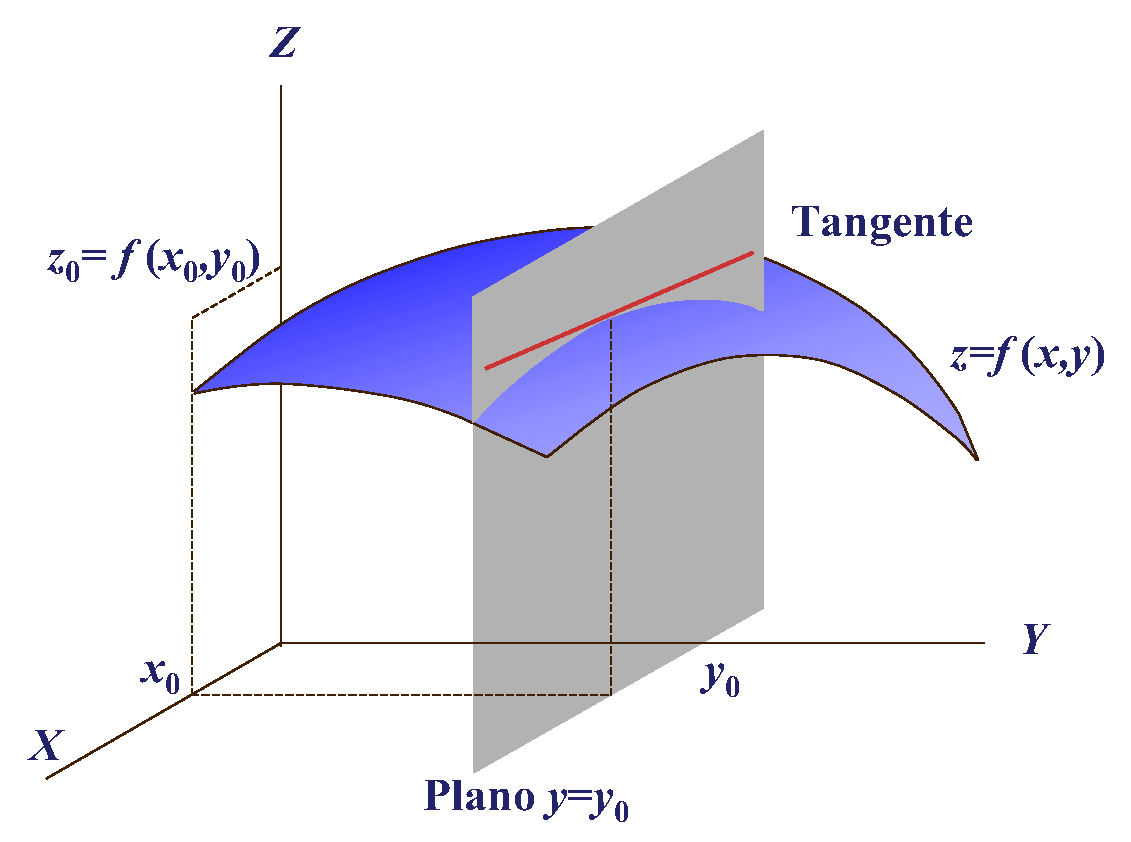
\includegraphics[scale=0.4]{img/tangentesuperficie}
	\end{center}
\end{frame}


%---------------------------------------------------------------------slide----
\begin{frame}
	\frametitle{Derivada parcial}
	El concepto de derivada parcial visto para funciones de dos variables puede extenderse fácilmente para funciones de $n$
	variables.
	
	\begin{definicion}[Derivada parcial]
		Dada una función de $n$ variables $f(x_1,\ldots,x_n)$, se dice que $f$ es \emph{derivable parcialmente} con respecto a
		la variable $x_i$ en el punto $a=(a_1,\ldots,a_n)$ si existe el límite
		\[
			\lim_{h\rightarrow 0} \frac{f(a_1,\ldots,a_{i-1},a_i+h,a_{i+1},\ldots,a_n)-f(a_1,\ldots,a_{i-1},a_i,a_{i+1},\ldots,a_n)} {h}.
		\]
		En tal caso, al valor del límite se le llama \emph{derivada parcial} de $f$ en $a$ con respecto a la variable $x_i$, y
		se denota
		\[
			f'_{x_i}(a)=\frac{\partial f}{\partial x_i}(a).
		\]
	\end{definicion}
	\structure{\bf Observación}
	La definición de derivada para funciones de una variable es un caso particular de esta definición para $n=1$.
\end{frame}


%---------------------------------------------------------------------slide----
\begin{frame}
	\frametitle{Cálculo de la derivada parcial}
	Al medir la variación de $f$ con respecto a la variación de una sola de sus variables $x_i$ en un punto
	$a=(a_1,\ldots,a_n)$, el resto de las variables se pueden considerar como constantes y, en tal caso, podemos ver a $f$
	como una función parcial $i$-ésima 
	\[
		f_i(x_i)=f(a_1,\ldots,a_{i-1},x_i,a_{i+1},\ldots,a_n).
	\]
	
	La derivada parcial de $f$ con respecto a $x_i$ puede calcularse derivando esta función:
	\[
		\frac{\partial f}{\partial x_i}(a)=f_i'(a_i).
	\]
	
	\begin{block}{Regla}
		Para derivar parcialmente $f(x_1,\ldots,x_n)$ con respecto a una variable $x_i$, se deriva $f$ como si la única variable
		fuese $x_i$, tratando el resto de las variables como constantes.
	\end{block} 
\end{frame}


%---------------------------------------------------------------------slide----
\begin{frame}
	\frametitle{Cálculo de la derivada parcial}
	\framesubtitle{Ejemplo con el volumen de un gas perfecto}
	En la ecuación de estado de los gases perfectos, el volumen es una función que depende de dos variables  
	\[v(t,p)=\frac{nRt}{p},\]
	donde $t$ mide la temperatura, $p$ la presión y $n$ y $R$ son constantes.
	
	La tasa de variación instantánea que experimenta el volumen con respecto a la presión viene dada por la derivada parcial de $v$ con respecto a $p$.
	
	Para calcular esta derivada parcial se fija $t$ como constante y se deriva $v$ como si la única variable fuese $p$:
	\[
		\frac{\partial v}{\partial p}(t,p)=\frac{d}{dp}\left(\frac{nRt}{p}\right)_{\mbox{\scriptsize $t=$cte}}=\frac{-nRt}{p^2}.
	\]
	
	Del mismo modo, la tasa de variación instantánea del volumen con respecto a la temperatura es:
	\[
		\frac{\partial v}{\partial t}(t,p)=\frac{d}{dt}\left(\frac{nRt}{p}\right)_{\mbox{\scriptsize$p=$cte}}=\frac{nR}{p}.
	\]
\end{frame}



\subsection{Vector gradiente}
%---------------------------------------------------------------------slide----
\begin{frame}
	\frametitle{Vector gradiente}
	\begin{definicion}[Vector gradiente]
		Dado un campo escalar $f(x_1,\ldots,x_n)$, se llama \emph{gradiente} de $f$, y se escribe $\nabla f$, a la función que a
		cada punto $a=(a_1,\ldots,a_n)$ le asigna el vector cuyas coordenadas cartesianas son las derivadas parciales de $f$ en
		$a$,
		\[
			\nabla f(a)=\left(\frac{\partial f}{\partial x_1}(a),\ldots,\frac{\partial f}{\partial x_n}(a)\right).
		\]
	\end{definicion}
	
	Más adelante se mostrará que vector gradiente en un punto dado tiene la misma magnitud y dirección que la velocidad máxima de variación de la
	función en ese punto. 
	
	De este modo, \alert{\emph{$\nabla f(a)$ indica la dirección de máximo crecimiento de $f$ en el punto $a$}}, mientras que $- \nabla f(a)$ indica la dirección de máximo decrecimiento.
\end{frame}



% ---------------------------------------------------------------------slide----
\begin{frame}
	\frametitle{Cálculo del vector gradiente}
	\framesubtitle{Ejemplo con una función de temperatura}
	Al calentar una superficie la temperatura $t$ (en ºC) en cada punto $(x,y,z)$ (en m) de dicha superficie viene dada por
	la función:
	\[ 
		t(x,y,z)=\frac{x}{y}+z^2. 
	\]
	\emph{¿En qué dirección y con qué magnitud aumentará más rápidamente la temperatura en el punto $(2,1,1)$ de dicha superficie?}
	
	
	La dirección en la que más rápidamente aumenta la temperatura nos la da el vector gradiente 
	\[
		\nabla t(x,y,z)=\left(\frac{\partial t}{\partial x}(x,y,z),\frac{\partial t}{\partial y}(x,y,z),\frac{\partial t}{\partial
			z}(x,y,z)\right)=\left(\frac{1}{y},\frac{-x}{y^2},2z\right).
	\]
	
	En el punto $(2,1,1)$ dicha dirección será
	\[
		\nabla t(2,1,1)=\left(\frac{1}{1},\frac{-2}{1^2},2\cdot 1\right)=(1,-2,2),
	\]
	y su magnitud 
	\[
		|\nabla f(2,1,1)|=|\sqrt{1^2+(-2)^2+2^2}|=|\sqrt{9}|=3 \mbox{ $^\circ$C/m}.
	\]
\end{frame}



\subsection{Composición de una trayectoria con un campo escalar}
%---------------------------------------------------------------------slide----
\begin{frame}
	\frametitle{Composición de una trayectoria con un campo escalar. Regla de la cadena}
	Si $f:\mathbb{R}^n\rightarrow \mathbb{R}$ es un campo escalar y $g:\mathbb{R}\rightarrow \mathbb{R}^n$ es una
	trayectoría, entonces es posible componer $g$ con $f$, de manera que $f\circ g:\mathbb{R}\rightarrow \mathbb{R}$ es una
	función real de variable real.
	
	La regla de la cadena para derivar la composición de una trayectoria con un campo escalar dice 
	\[
		(f\circ g)'(t) = \nabla f(g(t))\cdot g'(t) 
	\]  
\end{frame}


%---------------------------------------------------------------------slide----
\begin{frame}
	\frametitle{Composición de una trayectoria con un campo escalar. Regla de la cadena}
	\framesubtitle{Ejemplo}
	Si se toma el campo escalar del plano real $f(x,y)=x^2y$ y la trayectoria $g(t)=(\cos t,\sen t)$ $t\in [0,2\pi]$ del mismo plano, entonces
	\[
		\nabla f(x,y) = (2xy, x^2) \quad  \mbox{y} \quad g'(t) = (-\sen t, \cos t),
	\]
	y 
	\begin{align*}
		(f\circ g)'(t) & = \nabla f(g(t))\cdot g'(t) = (2\cos t\sen t,\cos^2 t)\cdot (-\sen t,\cos t) = \\
		               & = -2\cos t\sen^2 t+\cos^3 t.                                                   
	\end{align*}
	
	Se puede llegar al mismo resultado, sin aplicar la regla de la cadena, derivando directamente la función compuesta
	\[
		(f\circ g)(t) = f(g(t)) = f(\cos t, \sen t) = \cos^2 t\sen t,
	\]
	de manera que
	\[
		(f\circ g)'(t) = 2\cos t(-\sen t)\sen t+\cos^2 t \cos t = -2\cos t\sen^2 t+\cos^3 t.
	\]
\end{frame}


%---------------------------------------------------------------------slide----
\begin{frame}
	\frametitle{Composición de una trayectoria con un campo escalar. Regla de la cadena}
	La regla de la cadena para la composición de un campo escalar con una trayectoria permite obtener fácilmente el álgebra de derivadas para funciones reales de una variable real:
	\begin{align*}
		(u+v)'                    & = u'+v'               \\
		(uv)'                     & = u'v+uv'             \\
		\left(\frac{u}{v}\right)' & = \frac{u'v-uv'}{v^2} \\
		(u\circ v)'               & = u'(v)v'             
	\end{align*}
	
	Para deducir la derivada de la suma se toma el campo escalar $f(x,y)=x+y$ y la trayectoria $g(t)=(u(t),v(t))$, de manera que aplicando la regla de la cadena se tiene
	\[
		(u+v)'(t) = (f\circ g)'(t) = \nabla f(g(t))\cdot g'(t) = (1,1)\cdot (u'(t),v'(t)) = u'(t)+v'(t).
	\]
	y para deducir derivada del producto, tomando $f(x,y)=xy$, se tiene
	\[
		(uv)'(t) = (f\circ g)'(t) = \nabla f(g(t))\cdot g'(t) = (v(t),u(t))\cdot (u'(t),v'(t)) = u'(t)v(t)+u(t)v'(t).
	\]
\end{frame}



\subsection{Derivada direccional}
%---------------------------------------------------------------------slide----
\begin{frame}
	\frametitle{Derivada direccional}
	Para un campo escalar $f(x,y)$ de $\mathbb{R}^2$ y un punto $P=(x_0,y_0)$, se vió que $\dfrac{\partial f}{\partial x}$
	es la tasa de variación instantánea de $f$ con respecto a $x$ en el punto $P$, es decir, cuando nos desplazamos desde el
	punto $P$ en la dirección del eje $X$.
	
	Del mismo modo, $\dfrac{\partial f}{\partial y}$ es la tasa de variación instantánea de $f$ con respecto a $y$ en el
	punto $P$, es decir, cuando nos desplazamos desde el punto $P$ en la dirección del eje $Y$.
	
	Pero, \emph {¿qué pasa si nos movemos en cualquier otra dirección?}
	
	La tasa de variación instantánea de $f$ en un punto $P$ en la dirección de un vector unitario cualquiera $u$ se conoce como \emph{derivada direccional}.
	
\end{frame}


%---------------------------------------------------------------------slide----
\begin{frame}
	\frametitle{Derivada direccional}
	\begin{definicion}[Derivada direccional]
		Dado un campo escalar $f$ de $\mathbb{R}^n$, un punto $P$ y un vector unitario $\mathbf{u}$ en ese espacio, el límite
		\[
			f'_{\mathbf{u}}(P) = \lim_{h\rightarrow 0}\frac{f(P+h\mathbf{u})-f(P)}{h},
		\] 
		cuando existe, se llama \emph{derivada direccional} de $f$ en el punto $P$ en la dirección de $\mathbf{u}$.
	\end{definicion}
	Si se considera un vector unitario $\mathbf{u}$, la trayectoria que pasa por $P$, dirigida por $\mathbf{u}$, tiene ecuación
	\[
		g(t)=P+t\mathbf{u},\ t\in\mathbb{R},
	\]
	que para $t=0$, pasa por $P=g(0)$ con velocidad $\mathbf{u}=g'(0)$.
	
	Así, la tasa de variación de $f$ a partir del punto $P$ en la dirección de $\mathbf{u}$ es
	\[
		(f\circ g)'(0) = \nabla f(g(0))\cdot g'(0) = \nabla f(P)\cdot \mathbf{u}.
	\]
	
	Obsérvese que las derivadas parciales son las derivadas direccionales en las direcciones de los vectores coordenados. 
\end{frame}


%---------------------------------------------------------------------slide----
\begin{frame}
	\frametitle{Cálculo de la derivada direccional}
	\framesubtitle{Ejemplo}
	Dada la función $f(x,y) = x^2+y^2$, su vector gradiente es
	\[
		\nabla f(x,y) = (2x,2y),
	\]
	de manera que la derivada direccional en el punto $P=(1,1)$, en la dirección del vector unitario $\mathbf{u}=(1/\sqrt{2},1/\sqrt{2})$ es
	\[
		f'_{\mathbf{u}}(P) = \nabla f(P)\cdot \mathbf{u} = (2,2)\cdot(1/\sqrt{2},1/\sqrt{2}) = \frac{2}{\sqrt{2}}+\frac{2}{\sqrt{2}} = \frac{4}{\sqrt{2}}.
	\]
	
	Para calcular la derivada direccional en la dirección de un vector no unitario $\mathbf{v}$, basta con convertirlo en unitario mediante la transformación
	\[
		\mathbf{v'}=\frac{\mathbf{v}}{|\mathbf{v}|}.
	\] 
\end{frame}


%---------------------------------------------------------------------slide----
\begin{frame}
	\frametitle{Crecimiento de un campo escalar a partir del gradiente}
	Como se ha visto, para un vector unitario $\mathbf{u}$
	\[
		f'_{\mathbf{u}}(P) = \nabla f(P)\cdot \mathbf{u} = |\nabla f(P)|\cos \theta,
	\] 
	donde $\theta$ es el ángulo que forma $\mathbf{u}$ con el vector gradiente $\nabla f(P)$.
	
	Teniendo en cuenta que $-1\leq \cos\theta\leq 1$, para cualquier vector $\mathbf{u}$ se cumple 
	\[
		-|\nabla f(P)|\leq f'_{\mathbf{u}}(P)\leq |\nabla f(P)|.
	\]
	Además, si $\mathbf{u}$ tiene la misma dirección y sentido que el gradiente, se tiene $f'_{\mathbf{u}}(P)=|\nabla f(P)|\cos 0=|\nabla f(P)|$. 
	Por tanto, el \alert{\emph{crecimiento máximo de un campo escalar se produce en la dirección y sentido del gradiente}}.
	
	Del mismo modo, si $\mathbf{u}$ tiene la misma dirección y sentido opuesto al gradiente, se tiene $f'_{\mathbf{u}}(P)=|\nabla f(P)|\cos \pi=-|\nabla f(P)|$. 
	Por tanto, el \alert{\emph{decrecimiento máximo de un campo escalar se produce en la dirección y sentido opuesto al gradiente}}.  
\end{frame}


\subsection{Derivación implícita}
%---------------------------------------------------------------------slide----
\begin{frame}
	\frametitle{Derivación implícita}
	Si se sabe que la ecuación 
	\[
		f(x,y)=0
	\]
	define a $y$ como función de $x$, $y=h(x)$, alrededor de cierto valor $x=x_0$ para el que $y=h(x_0)=y_0$, entonces, si se toma la trayectoria $g(x)=(x,h(x))$, la ecuación anterior se puede expresar como
	\[
		(f\circ g)(x) = f(g(x)) = f(x,h(x))=0,
	\]
	de modo que usando la regla de la cadena sobre se tiene
	\[
		(f\circ g)'(x) = \nabla f(g(x))\cdot g'(x) = \left(\frac{\partial f}{\partial x}, \frac{\partial f}{\partial y}\right)\cdot (1,h'(x)) = 
		\frac{\partial f}{\partial x}+\frac{\partial f}{\partial y}h'(x) = 0,
	\] 
	de donde se deduce
	\[
		y'=h'(x)=\frac{-\dfrac{\partial f}{\partial x}}{\dfrac{\partial f}{\partial y}}
	\]
	A este proceso que permite obtener $y'$ en un entorno de $x_0$ sin disponer de la fórmula explícita $y=h(x)$, se le llama \emph{derivación implícita}.
\end{frame}


%---------------------------------------------------------------------slide----
\begin{frame}
	\frametitle{Derivación implícita}
	\framesubtitle{Ejemplo}
	La ecuación $x^2+y^2=1$ define a la circunferencia de radio 1 centrada en el origen de coordenadas, que también puede expresarse como
	\[
		f(x,y) = x^2+y^2-1 = 0.
	\]
	Si se piensa en $y$ como función implícita de $x$, se tiene 
	\[
		y'=\frac{-\dfrac{\partial f}{\partial x}}{\dfrac{\partial f}{\partial y}} = \frac{-2x}{2y}=\frac{-x}{y}.
	\]
	Podría llegarse al mismo resultado, despejando $y$ de la ecuación de la circunferencia, 
	\[
		x^2+y^2=1 \Leftrightarrow y^2=1-x^2 \Leftrightarrow y= \pm\sqrt{1-x^2}.
	\]
	Si se toma la raíz positiva, que corresponde a la semicircunferencia superior, la derivada vale
	\[
		y' = \frac{1}{2\sqrt{1-x^2}}(-2x) = \frac{-x}{\sqrt{1-x^2}}, 
	\]
	que coincide con el resultado de la derivación implícita, teniendo en cuenta que $y=\sqrt{1-x^2}$.
\end{frame}


%---------------------------------------------------------------------slide----
\begin{frame}
	\frametitle{Propiedad del gradiente}
	\begin{teorema}
		Sea $C$ el conjunto de nivel de un campo escalar $f$ que incluye a un punto $P$. 
		Si $\mathbf{v}$ es la velocidad al pasar por $P$ de una trayectoria que circule por $C$, entonces
		\[
			\nabla f(P) \cdot \mathbf{v} = 0.
		\] 
		Es decir, el vector gradiente de $f$ en $P$ es normal a $C$ en $P$, siempre que no sea nulo.
	\end{teorema}
	\structure{\textbf{Demostración}}
	Si se considera una trayectoria $g(t)$ a lo largo del conjunto de nivel $C$ que pase por $P=g(t_0)$, de modo que $\mathbf{v}=g'(t_0)$, entonces 
	\[
		(f\circ g)(t) = f(g(t)) = f(P),
	\]
	que es constante para cualquier $t$, y al aplicar la regla de la cadena se tiene
	\[
		(f\circ g)'(t) = \nabla f(g(t))\cdot  g'(t) = 0,
	\]
	de modo que, cuanto $t=t_0$, se tiene 
	\[
		\nabla f(P)\cdot \mathbf{v} = 0.
	\]
\end{frame}


%---------------------------------------------------------------------slide----
\begin{frame}
	\frametitle{Rectas normal y tangente a una linea en el plano}
	Según el resultado anterior, la recta normal a una línea $f(x,y)=0$ en un punto $P=(x_0,y_0)$, tiene ecuación
	\[
		P+t\nabla f(P) = (x_0,y_0)+t\nabla f(x_0,y_0).
	\]
	\structure{\textbf{Ejemplo}}
	Dado el campo escalar $f(x,y)=x^2+y^2-1$, y el punto $P=(0,1)$, resulta que el conjunto de nivel que pasa por $P$, para el que $f(x,y)=f(P)=0$ es la circunferencia de radio 1 centrada en el origen.
	Así pues, tomando como vector normal el gradiente de $f$
	\[
		\nabla f(x,y) = (2x,2y),
	\] 
	que en el punto $P=(0,1)$ vale $\nabla f(0,1) = (0,2)$, la recta normal a la circunferencia en $P$ es
	\[
		P+t\nabla f(P) = (0,1)+t(0,2) = (0,1+2t),
	\]
	que se trata de la recta vertical $x=0$, que coincide con el eje $Y$.
	
	y la recta tangente a la circunferencia en $P$ es
	\[
		((x,y)-P)\cdot \nabla f(P) = ((x,y)-(0,1))\cdot (0,2) = (x,y-1)\cdot(0,2) = 2(y-1) = 0 \Rightarrow y=1. 
	\]
\end{frame}


%---------------------------------------------------------------------slide----
\begin{frame}
	\frametitle{Recta normal y plano tangente a una superficie}
	De mismo modo, si en lugar de una línea en el plano se tiene una superficie $f(x,y,z)=0$, en el punto $P=(x_0,y_0,z_0)$ la recta normal tiene ecuación
	\[
		P+t\nabla f(P) = (x_0,y_0,z_0)+t\nabla f(x_0,y_0,z_0).
	\]
	\structure{\textbf{Ejemplo}}
	Dada el campo escalar $f(x,y,z)=x^2+y^2-z$, y el punto $P=(1,1,2)$, resulta que el conjunto de nivel que pasa por $P$, para el que $f(x,y)=f(P)=0$, es el paraboloide $z=x^2+y^2$.
	Así pues, tomando como vector normal el gradiente de $f$, que vale  
	\[
		\nabla f(x,y,z) = (2x,2y,-1),
	\] 
	que en el punto $P=(1,1,2)$ vale $\nabla f(1,1,2) = (2,2,-1)$, la recta normal al paraboloide en $P$ es
	\[
		P+t\nabla f(P) = (1,1,2)+t\nabla f(1,1,2) = (1,1,2)+t(2,2,-1) = (1+2t,1+2t,2-t),
	\]
	que se trata de la recta de ecuaciones  $x=y$ y $x=5-2z$.
	
	Y el plano tangente al paraboloide en $P$ es
	\begin{align*}
		((x,y,z)-P)\cdot \nabla f(P) & = ((x,y,z)-(1,1,2))(2,2,-1) = (x-1,y-1,z-2)(2,2,-1)= \\
		                             & = 2(x-1)+2(y-1)-(z-2) = 2x+2y-z-2= 0.                
	\end{align*}
\end{frame}


%---------------------------------------------------------------------slide----
\begin{frame}
	\frametitle{Recta normal y plano tangente a una superficie}
	\framesubtitle{Ejemplo}
	La gráfica del paraboloide $f(x,y,z)=x^2+y^2-z=0$ y su plano tangente en el punto $P=(1,1,2)$ es 
	\begin{center}
		\scalebox{1}{\psset{unit=0.7}
\psset{viewpoint=50 -40 30 rtp2xyz,Decran=60}
\begin{pspicture*}(-7,-2)(7,5.5)
\psSurface[fillcolor=red!50,ngrid=.25 .25,incolor=yellow,algebraic,linewidth=0.25\pslinewidth,linecolor=gray](-1.5,-1.5)(2,2){2*x+2*y-2}
\psSurface[fillcolor=blue!50,ngrid=.25 .25,incolor=yellow,algebraic,linewidth=0.25\pslinewidth,linecolor=gray](-1.5,-1.5)(1.5,1.5){x^2+y^2}
\axesIIID(0,0,2)(2,2,5)
\psPoint(1,1,2){p}
\psdots[linecolor=red](p)
\uput[r](p){$(1,1,2)$}
\end{pspicture*}}
	\end{center}
\end{frame}


\subsection{Derivadas parciales de segundo orden}
%---------------------------------------------------------------------slide----
\begin{frame}
	\frametitle{Derivadas parciales de segundo orden}
	Las derivadas parciales de una función son, a su vez, funciones de varias variables que muchas veces pueden volverse a
	derivar parcialmente con respecto a alguna de sus variables. 
	
	Si una función $f(x_1,\ldots,x_n)$ tiene derivada parcial $f'_{x_i}(x_1,\ldots,x_n)$ con respecto a la variable $x_i$ en un conjunto $A$, entonces podemos derivar de nuevo parcialmente $f'_{x_i}$ con respecto a la variable $x_j$. Esta segunda derivada, cuando existe, se llama \emph{derivada parcial de segundo orden} de $f$ con respecto a las variables $x_i$ y $x_j$, y se nota
	\[
		\frac{\partial ^2 f}{\partial x_j \partial x_i}= \frac{\partial}{\partial x_j}\left(\frac{\partial f}{\partial x_i}\right).
	\]
	
	De forma análoga se definen las derivadas de orden superior.
\end{frame}


%---------------------------------------------------------------------slide----
\begin{frame}
	\frametitle{Cálculo de las derivadas parciales de segundo orden}
	La función de dos variables
	\[f(x,y)=x^y\]
	tiene cuatro derivadas parciales de segundo orden, que son:
	\begin{align*}
		\frac{\partial^2 f}{\partial x^2}(x,y)          & = 
		\frac{\partial}{\partial x}\left(\frac{\partial f}{\partial x}(x,y)\right) =
		\frac{\partial}{\partial x}\left(yx^{y-1}\right) =
		y(y-1)x^{y-2},\\
		\frac{\partial^2 f}{\partial y \partial x}(x,y) & = 
		\frac{\partial}{\partial y}\left(\frac{\partial f}{\partial x}(x,y)\right) =
		\frac{\partial}{\partial y}\left(yx^{y-1}\right) =
		x^{y-1}+yx^{y-1}\log x,\\
		\frac{\partial^2 f}{\partial x \partial y}(x,y) & = 
		\frac{\partial}{\partial x}\left(\frac{\partial f}{\partial y}(x,y)\right) =
		\frac{\partial}{\partial x}\left(x^y\log x \right) =
		yx^{y-1}\log x+x^y\frac{1}{x},\\
		\frac{\partial^2 f}{\partial y^2}(x,y)          & = 
		\frac{\partial}{\partial y}\left(\frac{\partial f}{\partial y}(x,y)\right) =
		\frac{\partial}{\partial y}\left(x^y\log x \right) =
		x^y(\log x)^2.
	\end{align*}
\end{frame}


\subsection{Matriz hessiana}
%---------------------------------------------------------------------slide----
\begin{frame}
	\frametitle{Matriz hessiana y f hessiano}
	\begin{definicion}[Matriz hessiana]
		Dada una función de varias variables $f(x_1,\ldots,x_n)$, para la que existen todas sus derivadas parciales de segundo
		orden en un punto $a=(a_1,\ldots,a_n)$, se define la \emph{matriz hessiana} de $f$ en $a$, y se nota $\nabla^2f(a)$, como la
		matriz cuadrada cuyos elementos son
		\[
			\nabla^2f(a)=\left(
			\begin{array}{cccc}
				\dfrac{\partial^2 f}{\partial x_1^2}(a) & 
				\dfrac{\partial^2 f}{\partial x_1 \partial x_2}(a) &
				\cdots &
				\dfrac{\partial^2 f}{\partial x_1 \partial x_n}(a)\\
				\dfrac{\partial^2 f}{\partial x_2 \partial x_1}(a) &
				\dfrac{\partial^2 f}{\partial x_2^2}(a) & 
				\cdots &
				\dfrac{\partial^2 f}{\partial x_2 \partial x_n}(a)\\
				\vdots & \vdots & \ddots & \vdots \\
				\dfrac{\partial^2 f}{\partial x_n \partial x_1}(a) &
				\dfrac{\partial^2 f}{\partial x_n \partial x_2}(a) &
				\cdots &
				\dfrac{\partial^2 f}{\partial x_n^2}(a)
			\end{array}
			\right)
		\]
		Al determinante de esta matriz se le llama \emph{hessiano} de $f$ en $a$, y se nota $Hf(a)=|\nabla^2f(a)|$.
	\end{definicion}
\end{frame}


%---------------------------------------------------------------------slide----
\begin{frame}
	\frametitle{Cálculo de la matriz hessiana y el hessiano}
	Consideremos de nuevo la función de dos variables
	\[f(x,y)=x^y.\]
	Su matriz hessiana es:
	\[
		\nabla^2f(x,y)=\left(
		\begin{array}{cc}
			\dfrac{\partial^2 f}{\partial x^2}          & \dfrac{\partial^2 f}{\partial x \partial y} \\
			\dfrac{\partial^2 f}{\partial y \partial x} & \dfrac{\partial^2 f}{\partial y^2}          
		\end{array}
		\right)
		=
		\left(
		\begin{array}{cc}
			y(y-1)x^{y-2}      & x^{y-1}(y\log x+1) \\
			x^{y-1}(y\log x+1) & x^y(\log x)^2      
		\end{array}
		\right).
	\]
	
	En el punto $(1,2)$ la matriz vale
	\[
		\nabla^2f(1,2)=\left(
		\begin{array}{cc}
			2(2-1)1^{2-2}      & 1^{2-1}(2\log 1+1) \\
			1^{2-1}(2\log 1+1) & 1^2(\log 1)^2      
		\end{array}
		\right)
		=
		\left(
		\begin{array}{cc}
			2 & 1 \\
			1 & 0 
		\end{array}
		\right).
	\]
	
	Y el hessiano en dicho punto vale
	\[ 
		Hf(1,2)=\left|
		\begin{array}{cc}
			2 & 1 \\
			1 & 0 
		\end{array}
		\right|=
		2\cdot 0-1\cdot1= -1.
	\]
\end{frame}


%---------------------------------------------------------------------slide----
\begin{frame}
	\frametitle{Igualdad de las derivadas cruzadas}
	En el ejemplo anterior se aprecia que las \emph{derivadas cruzadas} de segundo orden $\frac{\partial^2 f}{\partial y\partial x}$ y $\frac{\partial^2 f}{\partial x\partial y}$ coinciden. Ello es debido al siguiente teorema: 
	
	\begin{teorema}[Igualdad derivadas cruzadas]
		Si $f(x,y)$ es una función tal que sus derivadas parciales $\frac{\partial f}{\partial x}$, $\frac{\partial f}{\partial y}$, $\frac{\partial^2 f}{\partial y\partial x}$ y $\frac{\partial^2 f}{\partial x\partial y}$ existen y son continuas en un conjunto abierto $A$, entonces
		\[
			\frac{\partial^2 f}{\partial y\partial x}=\frac{\partial^2 f}{\partial x\partial y}.
		\]
	\end{teorema}
	
	Una consecuencia del teorema es que, al calcular una derivada parcial de segundo orden que cumpla lo anterior, \alert{\emph{¡el orden en que se realicen las derivadas parciales no importa!}}
	
	Si el teorema se cumple para todas las derivadas parciales de segundo orden, entonces la matriz hessiana es simétrica. 
\end{frame}



\subsection{Fórmula de Taylor}
%---------------------------------------------------------------------slide----
\begin{frame}
	\frametitle{Aproximación lineal de un campo escalar}
	Ya se vio cómo aproximar funciones de una variable mediante polinomios de Taylor. 
	Esto también se puede generalizar a la aproximación de campos escalares mediante polinomios de varias variables. 
	
	Si $P$ es un punto del dominio de un campo escalar $f$ y $\mathbf{v}$ un vector, la \emph{fórmula de Taylor} de primer grado de $f$ alrededor del punto $P$ es
	\[
		f(P+\mathbf{v}) = f(P) + \nabla f(P)\cdot \mathbf{v} +R^1_{f,P}(\mathbf{v}),
	\]
	donde 
	\begin{align*}
		P^1_{f,P}(\mathbf{v}) = f(P)+\nabla f(P)\mathbf{v} 
	\end{align*}
	es el \emph{polinomio de Taylor} de primer grado de $f$ en el punto $P$, y $R^1_{f,P}(\mathbf{v})$ es el \emph{resto de taylor} para el vector $\mathbf{v}$, y mide el error cometido en la aproximación.
	
	Se cumple que  
	\[
		\lim_{|\mathbf{v}|\rightarrow 0} \frac{R^1_{f,P}(\mathbf{v})}{|\mathbf{v}|} = 0
	\]
	
	Obsérvese que el polinomio de Taylor de primer grado coincide con el plano tangente a $f$ en $P$.
\end{frame}


%---------------------------------------------------------------------slide----
\begin{frame}
	\frametitle{Aproximación lineal de un campo escalar}
	\framesubtitle{Campo escalar de dos variables}
	Si $f$ es un campo escalar de dos variables $f(x,y)$ y $P=(x_0,y_0)$, teniendo en cuenta que para un punto cualquiera $Q=(x,y)$, el vector $\mathbf{v}=\vec{PQ}=(x-x_0,y-y_0)$, el polinomio de Taylor de $f$
	en el punto $P$, puede expresarse
	\begin{align*}
		P^1_{f,P}(x,y) & = f(x_0,y_0)+\nabla f(x_0,y_0)(x-x_0,y-y_0) =                                                             \\
		               & = f(x_0,y_0)+\frac{\partial f}{\partial x}(x_0,y_0)(x-x_0)+\frac{\partial f}{\partial y}(x_0,y_0)(y-y_0). 
	\end{align*}
\end{frame}


%---------------------------------------------------------------------slide----
\begin{frame}
	\frametitle{Aproximación lineal de un campo escalar}
	\framesubtitle{Ejemplo}
	Dado el campo escalar $f(x,y)=\log(xy)$, su gradiente es
	\[
		\nabla f(x,y) = \left(\frac{1}{x},\frac{1}{y}\right),
	\]
	y el polinomio de Taylor de primer grado en el punto $P=(1,1)$ es
	\begin{align*}
		P^1_{f,P}(x,y) & = f(1,1) +\nabla f(1,1)\cdot (x-1,y-1) =        \\
		               & = \log 1+(1,1)\cdot(x-1,y-1) = x-1+y-1 = x+y-2. \\
	\end{align*}
	Este polinomio, permite aproximar el valor de $f$ cerca del punto $P$.
	Por ejemplo
	\[ 
		f(1.01,1.01) \approx P^1_{f,P}(1.01,1.01) = 1.01+1.01-2 = 0.02.
	\]
\end{frame}


%---------------------------------------------------------------------slide----
\begin{frame}
	\frametitle{Aproximación cuadrática de un campo escalar}
	Si $P$ es un punto del dominio de un campo escalar $f$ y $\mathbf{v}$ un vector, la \emph{fórmula de Taylor} de segundo
	grado de $f$ alrededor del punto $P$ es
	\[
		f(P+\mathbf{v}) = f(P) + \nabla f(P)\cdot \mathbf{v} + \frac{1}{2}\nabla^2f(P)\mathbf{v}\cdot\mathbf{v} + R^2_{f,P}(\mathbf{v}),
	\]
	donde 
	\begin{align*}
		P^2_{f,P}(\mathbf{v}) & =f(P)+\nabla f(P)\mathbf{v}+\frac{1}{2}\nabla^2f(P)\mathbf{v}\cdot\mathbf{v} 
	\end{align*}
	es el \emph{polinomio de Taylor} de segundo grado de $f$ en el punto $P$, y $R^2_{f,P}(\mathbf{v})$ es el \emph{resto de taylor} para el vector $\mathbf{v}$.
	
	Se cumple que  
	\[
		\lim_{|\mathbf{v}\rightarrow 0|} \frac{R^2_{f,P}(\mathbf{v})}{|\mathbf{v}|^2} = 0
	\]
	lo que indica que el resto es mucho más pequeño que el cuadrado del módulo de $\mathbf{v}$.
\end{frame}


%---------------------------------------------------------------------slide----
\begin{frame}
	\frametitle{Aproximación cuadrática de un campo escalar}
	\framesubtitle{Campo escalar de dos variables}
	Si $f$ es un campo escalar de dos variables $f(x,y)$ y $P=(x_0,y_0)$, el polinomio de Taylor de $f$ en el punto $P$, puede expresarse
	\begin{multline*}
		P^2_{f,P}(x,y) = f(x_0,y_0)+\nabla f(x_0,y_0)(x-x_0,y-y_0) +\\
		+\frac{1}{2}(x-x_0,y-y_0)\nabla^2f(x_0,y_0)(x-x_0,y-y_0)= \\
		= f(x_0,y_0)+\frac{\partial f}{\partial x}(x_0,y_0)(x-x_0)+\frac{\partial f}{\partial y}(x_0,y_0)(y-y_0)+\\
		+\frac{1}{2}\left(\frac{\partial^2 f}{\partial x^2}(x_0,y_0) (x-x_0)^2 + 2\frac{\partial^2 f}{\partial y\partial x}(x_0,y_0) (x-x_0)(y-y_0) + \frac{\partial^2 f}{\partial y^2}(x_0,y_0) (y-y_0)^2\right)
	\end{multline*}
\end{frame}


%---------------------------------------------------------------------slide----
\begin{frame}
	\frametitle{Aproximación cuadrática de un campo escalar}
	\framesubtitle{Ejemplo}
	Dado el campo escalar $f(x,y)=\log(xy)$, su gradiente es
	\[
		\nabla f(x,y) = \left(\frac{1}{x},\frac{1}{y}\right),
	\]
	y su matriz hessiana es 
	\[
		Hf(x,y) = \left(
		\begin{array}{cc}
			\frac{-1}{x^2} & 0              \\
			0              & \frac{-1}{y^2} 
		\end{array}
		\right)
	\]
	y el polinomio de Taylor de segundo grado en el punto $P=(1,1)$ es
	\begin{align*}
		P^2_{f,P}(x,y) & = f(1,1) +\nabla f(1,1)\cdot (x-1,y-1) + \frac{1}{2}(x-1,y-1)\nabla^2f(1,1)\cdot(x-1,y-1)= \\
		               & = \log 1+(1,1)\cdot(x-1,y-1) + \frac{1}{2}(x-1,y-1)                                        
		\left(
		\begin{array}{cc}
		-1             & 0                                                                                          \\
		0              & -1                                                                                         
		\end{array}
		\right)
		\left(
		\begin{array}{c}
		x-1\\
		y-1
		\end{array}
		\right)
		= \\
		               & = x-1+y-1+\frac{-x^2-y^2+2x+2y-2}{2} = \frac{-x^2-y^2+4x+4y-6}{2}.                         
	\end{align*}
	Así, $f(1.01,1.01) \approx P^1_{f,P}(1.01,1.01) = \frac{-1.01^2-1.01^2+4\cdot 1.01+4\cdot 1.01-6}{2} = 0.0199$.
\end{frame}


\subsection{Extremos}
%---------------------------------------------------------------------slide----
\begin{frame}
	\frametitle{Extremos de un campo escalar}
	\begin{definicion}[Máximo y mínimo relativos]
		Dado un campo escalar $f$ de $\mathbb{R}^n$, se dice que un punto $P$ es un \emph{máximo relativo} de $f$ si existe un valor $\epsilon>0$ tal que
		\[
			f(P)\geq f(X)\ \forall X, |\vec{PX}|<\epsilon.
		\] 
		Del mismo modo se dice que un punto $P$ es un \emph{mínimo relativo} de $f$ si existe un valor $\epsilon>0$ tal que
		\[
			f(P)\leq f(X)\ \forall X, |\vec{PX}|<\epsilon.
		\] 
		A los máximos y mínimos de $f$ se les conoce como \emph{extremos relativos} de $f$.
	\end{definicion}
\end{frame}


%---------------------------------------------------------------------slide----
\begin{frame}
	\frametitle{Anulación del gradiente en los extremos}
	\begin{teorema}
		Si $P$ es un extremo de un campo escalar $f$ de $\mathbb{R}^n$, entonces $P$ es un punto crítico de $f$, es decir,
		\[
			\nabla f(P) = 0.
		\]
	\end{teorema}
	
	\structure{\textbf{Demostración}} Tomando la trayectoria que pasa por $P$ con la dirección y sentido del gradiente,
	\[
		g(t)=P+t\nabla f(P),
	\] 
	la función $h=(f\circ g)(t)$ no decrece en $t=0$ ya que 
	\[
		h'(0)= (f\circ g)'(0) = \nabla f(g(0))\cdot g'(0) = \nabla f(P)\cdot \nabla f(P) = |\nabla f(P)|^2\geq 0.
	\]
	y sólo se anula si $\nabla f(P)=0$.
	
	Así pues, si $\nabla f(P)\neq 0$, entonces $P$ no puede ser un máximo ya que siguiendo la trayectoria de $g$ desde $P$ se encontrarían puntos en los que la imagen de $f$ es mayor que en $P$.
	Del mismo modo, siguiendo la trayectoria opuesta a $g$ se encontrarían puntos en los que la imagen de $f$ es menor que la imagen en $P$, por lo que tampoco puede ser un mínimo. 
\end{frame}


%---------------------------------------------------------------------slide----
\begin{frame}
	\frametitle{Anulación del gradiente en los extremos}
	\framesubtitle{Ejemplo}
	Para el campo escalar $f(x,y)=x^2+y^2$, resulta evidente que sólo tiene un mínimo en el origen $(0,0)$ ya que 
	\[
		f(0,0)=0 \leq f(x,y)=x^2+y^2,\ \forall x,y\in \mathbb{R}.
	\]
	En este punto se cumple, $\nabla f(0,0) = 0$.
	\begin{center}
		\scalebox{1}{\psset{unit=0.7}
\psset{viewpoint=50 30 30 rtp2xyz,Decran=60}
\begin{pspicture*}(-7,-3)(7,5.5)
\psSurface[fillcolor=blue!50,ngrid=.25 .25,incolor=yellow,algebraic,linewidth=0.25\pslinewidth,linecolor=gray](-1.5,-1.5)(1.5,1.5){x^2+y^2}
\axesIIID(0,0,2)(2,2,5)
\psPoint(0,0,0){p}
\psdots[linecolor=red](p)
\uput[r](p){$(0,0,0)$}
\end{pspicture*}}
	\end{center}
\end{frame}


%---------------------------------------------------------------------slide----
\begin{frame}
	\frametitle{Puntos de silla}
	No todos los puntos críticos son extremos. 
	Si se considera, por ejemplo, el campo escalar $f(x,y)=x^2-y^2$, su gradiente es
	\[
		\nabla f(x,y) = (2x,-2y),
	\]
	que sólo se anula en el punto $(0,0)$. 
	Sin embargo, este punto no es un máximo relativo ya que los puntos $(x,0)$ del eje $X$ tienen imágenes $f(x,0)=x^2\geq
	0=f(0,0)$, y tampoco es un mínimo relativo ya que los puntos $(0,y)$ del eje $Y$ tienen imágenes $f(0,y)=-y^2\leq
	0=f(0,0)$.
	Este tipo de puntos que anulan el gradiente pero que no son extremos, se conocen como \emph{puntos de silla}.
	\begin{center}
		\scalebox{1}{\psset{unit=0.45}
\psset{viewpoint=50 50 30 rtp2xyz,Decran=50}
\begin{pspicture*}(-7,-4.3)(7,4.3)
%\psSolid[object=grille,base=-4 4 -4 4,action=draw]
\psSurface[fillcolor=blue!50,ngrid=.25 .25,incolor=yellow,algebraic,linewidth=0.25\pslinewidth,linecolor=gray](-2,-2)(2,2){x^2-y^2}
\axesIIID(1,0,0)(4,4,4)
\psPoint(0,0,0){p}
\psdots[linecolor=red](p)
\uput[r](p){$(0,0,0)$}
\end{pspicture*}}
	\end{center}
\end{frame}


%---------------------------------------------------------------------slide----
\begin{frame}
	\frametitle{Determinación de los extremos de un campo escalar}
	De la fórmula de Taylor de segundo grado para un campo escalar $f$ en un punto $P$ se deduce que
	\[
		f(P+\mathbf{v})-f(P) \approx \nabla f(P)\mathbf{v}+\frac{1}{2}\nabla^2f(P)\mathbf{v}\cdot\mathbf{v}.
	\]
	De manera que si $P$ es un punto crítico de $f$, como $\nabla f(P)=0$, se tiene que 
	\[
		f(P+\mathbf{v})-f(P) \approx \frac{1}{2}\nabla^2f(P)\mathbf{v}\cdot\mathbf{v}.
	\]
	Por tanto, el signo de $f(P+\mathbf{v})-f(P)$ coincide con el signo del término cuadrático $\nabla^2f(P)\mathbf{v}\cdot\mathbf{v}$.
	
	Se pueden dar cuatro posibilidades:
	\begin{itemize}
		\item Definido positivo: $\nabla^2f(P)\mathbf{v}\cdot\mathbf{v}>0$ $\forall \mathbf{v}\neq 0$.
		\item Definido negativo: $\nabla^2f(P)\mathbf{v}\cdot\mathbf{v}<0$ $\forall \mathbf{v}\neq 0$.
		\item Indefinido: $\nabla^2f(P)\mathbf{v}\cdot\mathbf{v}>0$ para algún $\mathbf{v}\neq 0$ y  $\nabla^2f(P)\mathbf{u}\cdot\mathbf{u}<0$ para algún $\mathbf{u}\neq 0$.
		\item Semidefinido: Cualquier otro caso distinto de los anteriores.
	\end{itemize}
\end{frame}


%---------------------------------------------------------------------slide----
\begin{frame}
	\frametitle{Determinación de los extremos de un campo escalar}
	Así pues, dependiendo el signo de $Hf(P)\mathbf{v}\cdot\mathbf{v}$, se tiene
	\begin{teorema}
		Dado un punto crítico $P$ de un campo escalar $f$ que tiene matríz hessiana $Hf(P)$, se cumple
		\begin{itemize}
			\item Si $\nabla^2f(P)$ es definido positivo entonces $f$ tiene un mínimo relativo en $P$.
			\item Si $\nabla^2f(P)$ es definido negativo entonces $f$ tiene un máximo relativo en $P$.
			\item Si $\nabla^2f(P)$ es indefinido entonces $f$ tiene un punto de silla en $P$.
		\end{itemize}
	\end{teorema}
	En el caso de que $\nabla^2f(P)$ sea semidefinido, no se puede obtener ninguna conclusión y hay que recurrir a derivadas parciales de orden superior.
\end{frame}


%---------------------------------------------------------------------slide----
\begin{frame}
	\frametitle{Determinación de los extremos de un campo escalar}
	\framesubtitle{Campo escalar de dos variables}
	En el caso particular de un campo escalar de dos variables se tiene
	\begin{teorema}
		Dado un punto crítico $P=(x_0,y_0)$ de un campo escalar $f(x,y)$ que tiene matríz hessiana $\nabla^2f(P)$, se cumple
		\begin{itemize}
			\item Si $Hf(P)>0$ y $\dfrac{\partial^2 f}{\partial x^2}(x_0,y_0)>0$ entonces $f$ tiene un mínimo relativo en $P$.
			\item Si $Hf(P)>0$ y $\dfrac{\partial^2 f}{\partial x^2}(x_0,y_0)<0$ entonces $f$ tiene un máximo relativo en $P$.
			\item Si $Hf(P)<0$ entonces $f$ tiene un punto de silla en $P$.
		\end{itemize}
	\end{teorema}
\end{frame}


%---------------------------------------------------------------------slide----
\begin{frame}
	\frametitle{Determinación de los extremos de un campo escalar}
	\framesubtitle{Ejemplo}
	Dada el campo escalar $f(x,y)=\dfrac{x^3}{3}-\dfrac{y^3}{3}-x+y$, se tiene que su gradiente vale
	\[
		\nabla f(x,y)= (x^2-1,-y^2+1),
	\]
	que se anula en los puntos $(1,1)$, $(1,-1)$, $(-1,1)$ y $(-1,-1)$.
	
	La matriz hessiana vale 
	\[
		\nabla^2f(x,y) = \left(
		\begin{array}{cc}
			2x & 0   \\
			0  & -2y 
		\end{array}
		\right)
	\]
	y el hessiano vale
	\[
		Hf(x,y) = -4xy.
	\]
	Así pues, se tiene
	\begin{itemize}
		\item Punto $(1,1)$: $Hf(1,1)=-4<0 \Rightarrow$ Punto de silla.
		\item Punto $(1,-1)$: $Hf(1,-1)=4>0$ y $\frac{\partial^2}{\partial x^2}(1,-1)=2>0 \Rightarrow$ Mínimo relativo.
		\item Punto $(-1,1)$: $Hf(-1,1)=4>0$ y $\frac{\partial^2}{\partial x^2}(-1,1)=-2<0 \Rightarrow$ Máximo relativo.
		\item Punto $(-1,-1)$: $Hf(-1,-1)=-4<0 \Rightarrow$ Punto de silla.
	\end{itemize}
\end{frame}


%---------------------------------------------------------------------slide----
\begin{frame}
	\frametitle{Determinación de los extremos de un campo escalar}
	\framesubtitle{Ejemplo}
	\begin{center}
		\scalebox{1}{\psset{unit=1}
\psset{viewpoint=50 50 30 rtp2xyz,Decran=50}
\begin{pspicture*}(-6,-4)(7,4.3)
%\psSolid[object=grille,base=-4 4 -4 4,action=draw]
\psSurface[fillcolor=blue!50,ngrid=.25 .25,incolor=yellow,algebraic,linewidth=0.25\pslinewidth,linecolor=gray](-2,-2)(2,2){x^3/3-y^3/3-x+y}
\axesIIID(0,1,0)(3,3,3)
\psPoint(1,1,0){p1}
\psPoint(1,-1,-1.34){p2}
\psPoint(-1,1,1.34){p3}
\psPoint(-1,-1,0){p4}
\psPoint(2,4,5){f}
\psdots[linecolor=red](p1)(p2)(p3)(p4)
\uput[r](f){$f(x,y)=\dfrac{x^3}{3}-\dfrac{y^3}{3}-x+y$}
\uput[r](p1){$(1,1,0)$}
\uput[d](p2){$(1,-1,-4/3)$}
\uput[r](p3){$(-1,1,4/3)$}
\uput[l](p4){$(-1,-1,0)$}
\end{pspicture*}}
	\end{center}
\end{frame}


% \section{Medida y Error}
%---------------------------------------------------------------------slide----
\mode<presentation>{
	\begin{frame}
		\frametitle{Medida y Error}
		\tableofcontents[sectionstyle=show/hide,hideothersubsections]
	\end{frame}
}


\subsection{Medida de una magnitud y error asociado}
%---------------------------------------------------------------------slide----
\begin{frame}
	\frametitle{Medidas}
	Cualquier ciencia experimental trata de conocer y comprender el mundo que estudia observándolo y realizando medidas
	experimentales.
	
	A partir de estas medidas se construirán y validarán los modelos matemáticos que expliquen los fenómenos naturales. En
	consecuencia, la bondad y calidad de estas medidas es fundamental a la hora de obtener modelos correctos.
	
	A la hora de realizar medidas experimentales de cualquier magnitud física, debe tenerse en cuenta que \emph{no existe
	ningún modo de medir una magnitud con infinita precisión} y por tanto, toda medida estará afectada de cierta
	\emph{imprecisión} o \emph{error}.
	
	\begin{block}{Medida de una magnitud}
		La medida de cualquier magnitud física $X$ debe expresarse indicando el mejor valor de la misma $x$ acompañado
		del error $\varepsilon$ de dicho valor:
		\[
			X = x\pm \varepsilon,
		\]
		donde $\varepsilon$ es una cota superior del error del valor $x$, es decir, $|X-x|\leq \varepsilon$.
	\end{block}
\end{frame}


%---------------------------------------------------------------------slide----
\begin{frame}
	\frametitle{Expresión de una medida y su error}
	A la hora de expresar una medida $X=x\pm \varepsilon$, deben tenerse en cuenta los siguientes criterios:
	\begin{itemize}
		\item El error $\varepsilon$ debe expresarse sólo con una o dos cifras significativas, donde la primera cifra
		      significativa de un número es la primera cifra distinta de cero comenzando por la izquierda, la segunda es la
		      siguiente, y así sucesivamente.
		      
		      Por tanto, \emph{el error debe redondearse por exceso en la primera o segunda cifra significativa}. 
		      
		\item El valor de la magnitud $x$ debe expresarse con tantas cifras significativas como indique su error y debe
		      redondearse, por exceso o por defecto, en la cifra significativa correspondiente a la última cifra considerada en el
		      error. 
	\end{itemize}
	
	\structure{\textbf{Ejemplo}} Si se mide la temperatura de un líquido y se obtiene un valor $186.27641$ K con un error
	$0.01638$ K, el resultado debe expresarse como
	\[
		T=186.276\pm 0.017 \mbox{ K}.
	\]
\end{frame}


%---------------------------------------------------------------------slide----
\begin{frame}
	\frametitle{Mejor valor de una magnitud}
	Siempre que sea posible las medidas de una magnitud deben repetirse para mejorar la precisión del resultado.
	
	Si se realizan $n$ mediciones de un mismo ente físico, todas ellas realizadas siguiendo un mismo procedimiento, se
	obtiene una muestra de medidas 
	\[
		x_1,x_2,\ldots, x_n.
	\]
	
	En principio, no hay ningún motivo para escoger uno u otro valor particular como mejor valor y por ello debe tomarse
	como mejor valor estimativo de la magnitud la \emph{media aritmética muestral} de los $n$ valores:
	\[
		\bar x = \frac{\sum_{i=1}^n x_i}{n}.
	\] 
\end{frame}



\subsection{Tipos de errores de una medida}
%---------------------------------------------------------------------slide----
\begin{frame}
	\frametitle{Tipos de errores asociados al mejor valor de una magnitud}
	Al medir una magnitud pueden aparecer distintos tipos de errores:
	\begin{itemize}
		\item Errores sistemáticos.
		\item Errores en el aparato de medida.
		\item Errores aleatorios o estadísticos.
	\end{itemize}
	El error total asociado al mejor valor de una magnitud será la suma de cada uno de estos tipos de errores. 
\end{frame}


%---------------------------------------------------------------------slide----
\begin{frame}
	\frametitle{Error sistemático}
	El \emph{error sistemático} $\varepsilon_{\textrm{sist}}$ es el debidos al método de medida utilizado. Suele
	deberse a la falta de calidad o calibrado del aparato de medida o a algún error o sesgo en la fórmula o diseño del
	experimento o a que la medición depende de la pericia del observador que mide.
	
	Afectan por igual a todas las medidas, haciendo que todas de ellas se desvíen en el mismo sentido, siendo por lo
	general difíles de dectectar y eliminar. Son, por lo tanto, los errores más indeseables y no existe ninguna expresión
	matemática que determine su valor, sino que deben ser estimados en cada caso según el método de medida utilizado.
	
	En el caso de errores debidos al calibrado del aparato, pueden eliminarse fácilmente haciendo una calibración del mismo
	antes de realizar las medidas. La calibración puede hacerse fácilmente midiendo una magnitud real de 0 y ajustando el
	aparato, si fuera necesario, para que efectivamente marque 0. 
\end{frame}


%---------------------------------------------------------------------slide----
\begin{frame}
	\frametitle{Error del aparato de medida }
	El \emph{error del aparato} $\Delta x$ es el debido al límite de precisión en la capacidad de medida del instrumento
	utilizado. 
	
	Este error, llamado también \emph{incertidumbre}, está siempre presente y es independiente del observador
	que realiza la medida.
	
	Cuando la escala del aparato no es continua, como ocurre en instrumentos digitales, la incertidumbre se toma igual a la
	mínima lectura que puede hacerse en dicha escala, y cuando es continua se toma igual a la mitad de la mínima lectura.
	
	\structure{\textbf{Ejemplo}} Si se mide el tiempo con un cronómetro digital con mínima unidad la décima de segundo,
	entonces la incertidumbre en las medidas será $\Delta t=0.1$ s, mientras que si se mide con un cronómetro analógico con
	movimiento continuo de la aguja, la incertidumbre será $\Delta t=0.05$ s.
\end{frame}


%---------------------------------------------------------------------slide----
\begin{frame}
	\frametitle{Error aleatorio}
	El \emph{error aleatorio} es el debido a las pequeñas variaciones incontrolables en las condiciones externas que se
	producen de unas medidas a otras, es decir, es el error debido al \emph{azar}. 
	
	Estos errores perturban de manera diferente a cada medida, explicando que se obtengan diferentes valores pese a que
	todas las observaciones se hagan siguiendo el mismo procedimiento o protocolo.
	
	En consecuencia, este error sólo tiene sentido cuando se realizan distintas medidas de una misma magnitud. 
\end{frame}


%---------------------------------------------------------------------slide----
\begin{frame}
	\frametitle{Cálculo del error aleatorio}
	Si se realizan $n$ mediciones, obteniendo los valores $x_1,\ldots,x_n$, entonces cada una de estas medidas puede
	expresarse como
	\[
		x_i = \mu + \varepsilon_i, 
	\]
	donde $\mu$ es la media poblacional de todas la medidas y $\varepsilon_i$ el error aleatorio asociado a cada medida.
	
	Como en el error aleatorio influyen multitud de factores debidos a azar, según el teorema central del límite puede
	afirmarse que $\varepsilon_i\sim N(0,\sigma)$, con $\sigma$ la desviación típica poblacional de todas las medidas, y que
	puede estimarse por medio de la
	\emph{cuasidesviación típica muestral}
	\[
		\hat{s}_x = \sqrt{\frac{\sum_{i=1}^n (x_i-\bar x)^2}{n-1}}, 
	\]
	
	Si, como hemos visto antes, se toma como mejor valor de la magnitud la media muestral $\bar x$, el error
	asociado será su desviación típica, que vale
	\[
		s_{\bar x} = \frac{\hat{s}_x}{\sqrt n} = \sqrt{\frac{\sum_{i=1}^n (x_i-\bar x)^2}{n(n-1)}}.
	\]
\end{frame}


%---------------------------------------------------------------------slide----
\begin{frame}
	\frametitle{Cálculo del error aleatorio}
	\framesubtitle{Ejemplo}
	Supongamos que al medir el periodo de oscilación de un péndulo con un cronómetro obtenemos las siguientes medidas:
	\begin{center}
		$1.21$s -- $1.19$s -- $1.22$s -- $1.18$s -- $1.19$s -- $1.20$s
	\end{center}
	
	Entonces el mejor valor del periodo del péndulo es 
	\[
		\bar x = \frac{1.21+1.19+1.22+1.18+1.19+1.20}{6} =  1.198333\mbox{s},
	\] 
	y el error debido al azar es
	\[
		s_{\bar x} = \sqrt{\frac{(1.21-1.198)^2+\cdots +(1.20-1.198)^2}{6\cdot 5}} = 0.006009\mbox{s}.
	\]
	Así pues, suponiendo que no haya error sistemático, la medida del periodo es, 
	\[
		1.198\pm 0.007\mbox{s}.
	\]
\end{frame}


%---------------------------------------------------------------------slide----
\begin{frame}
	\frametitle{Consideraciones sobre el error aleatorio}
	Puesto que el error aleatorio, si realmente depende del azar, debería seguir una distribución normal, entonces la media
	muestral $\bar x$ también seguirá una distribución normal
	\[
		\bar x\sim N(\mu,s_{\bar x}),
	\]
	de manera que, de acuerdo a la distribución normal se cumple
	\begin{itemize}
		\item $P(\bar x-s_{\bar x}\leq \mu\leq \bar x+s_{\bar x})=0.683$.
		\item $P(\bar x-2s_{\bar x}\leq \mu\leq \bar x+2s_{\bar x})=0.954$.
		\item $P(\bar x-3s_{\bar x}\leq \mu\leq \bar x+3s_{\bar x})=0.997$.
	\end{itemize}
	
	Por consiguiente, cuando se escribe $\bar x\pm s_{\bar x}$ no se está diciendo que el valor real está en el intervalo
	$(\bar x-s_{\bar x},\bar x+s_{\bar x})$, sino que existe aproximadamente un $68\%$ de probabilidad de que el valor real
	esté dentro del intervalo. 
	
	Otra consecuencia de esto mismo es que cuando una medida dista más de 3 veces la desviación típica de la media
	muestral, dicha medida debe descartarse ya que es muy probable que algo ha fallado en la medida. 
\end{frame}


%---------------------------------------------------------------------slide----
\begin{frame}
	\frametitle{Cálculo del error total}
	Según lo visto, el error total de una medida dependerá de si realizamos varias mediciones o sólo una.
	
	\begin{itemize}
		\item \structure{\textbf{Una medición}} Si sólo se realiza una medición, entonces el error aleatorio no tiene sentido y
		      el error total será la suma del error sistemático y el error del aparato, es decir,
		      \[
		      	\varepsilon = \varepsilon_{\textrm{sist}}+\Delta x.
		      \]
		\item \structure{\textbf{Varias mediciones}} Si se realizan varias mediciones, entonces el error total será la suma del
		      error sistemático, de la incertidumbre del aparato y del error aleatorio, es decir,
		      \[
		      	\varepsilon = \varepsilon_{\textrm{sist}}+\Delta x+s_{\bar x},
		      \]
		      aunque cuando se utilizan aparatos suficientemente precisos, la incertidumbre del aparto suele ser bastante menor que
		      el error aleatorio y puede despreciarse.
	\end{itemize} 
\end{frame}


%---------------------------------------------------------------------slide----
\begin{frame}
	\frametitle{Error sistemático vs error aleatorio}
	Utilizando el símil del tiro al blanco, tendríamos estas situaciones
	\begin{center}
		\scalebox{1}{\psset{unit=0.5}
\begin{pspicture*}(0,0)(18,14.5)
\footnotesize
\uncover<2->{
\pscircle[fillstyle=solid,fillcolor=red](4,12){2.5}
\pscircle[fillstyle=solid,fillcolor=white](4,12){2}
\pscircle[fillstyle=solid,fillcolor=red](4,12){1.5}
\pscircle[fillstyle=solid,fillcolor=white](4,12){1}
\pscircle[fillstyle=solid,fillcolor=red](4,12){0.5}
\psdots(4.1,12.1)(3.9,12.2)(3.8,12)(4,11.7)(4.2,11.8)(3.7,11.8)
\rput(4,9.1){Medidas sin error sistemático}
\rput(4,8.3){y error aleatorio pequeño}
}
\uncover<3->{
\pscircle[fillstyle=solid,fillcolor=red](14,12){2.5}
\pscircle[fillstyle=solid,fillcolor=white](14,12){2}
\pscircle[fillstyle=solid,fillcolor=red](14,12){1.5}
\pscircle[fillstyle=solid,fillcolor=white](14,12){1}
\pscircle[fillstyle=solid,fillcolor=red](14,12){0.5}
\psdots(15.1,12.1)(15.4,11)(13,11.9)(13.8,11.2)(14.5,13.2)(13,13.3)(14.2,12.1)
\rput(14,9.1){Medidas sin error sistemático}
\rput(14,8.3){y error aleatorio grande}
}
\uncover<4->{
\pscircle[fillstyle=solid,fillcolor=red](4,4){2.5}
\pscircle[fillstyle=solid,fillcolor=white](4,4){2}
\pscircle[fillstyle=solid,fillcolor=red](4,4){1.5}
\pscircle[fillstyle=solid,fillcolor=white](4,4){1}
\pscircle[fillstyle=solid,fillcolor=red](4,4){0.5}
\psdots(5.1,5.1)(4.9,5.2)(4.8,5)(5,4.7)(5.2,4.8)(3.7,11.8)(4.7,4.8)
\rput(4,1.1){Medidas con error sistemático}
\rput(4,0.3){y error aleatorio pequeño}
}
\uncover<5->{
\pscircle[fillstyle=solid,fillcolor=red](14,4){2.5}
\pscircle[fillstyle=solid,fillcolor=white](14,4){2}
\pscircle[fillstyle=solid,fillcolor=red](14,4){1.5}
\pscircle[fillstyle=solid,fillcolor=white](14,4){1}
\pscircle[fillstyle=solid,fillcolor=red](14,4){0.5}
\psdots(16.1,4.1)(16.4,3)(14,4.9)(14.8,4.2)(15.5,6.2)(14,6.3)(15.2,5.1)
\rput(14,1.1){Medidas con error sistemático}
\rput(14,0.3){y error aleatorio grande}
}
\end{pspicture*}}
	\end{center}
\end{frame}



\subsection{Error de las medidas indirectas}
%---------------------------------------------------------------------slide----
\begin{frame}
	\frametitle{Error de la medidas indirectas}
	Hay magnitudes para las que existe un aparato que permite medirlas directamente, como pueden ser la longitud, el
	tiempo, el volumen o la temperatura, mientras que otras deben ser medidas indirectamente a partir de una fórmula en la
	que intervienen medidas directas u otras indirectas calculadas previamente. Esto puede expresarse funcionalmente de la forma
	\[Y(X_1,\ldots,X_n),\]
	donde $Y$ es la magnitud medida indirectamente y $X_1,\ldots,X_n$ son las medias de las magnitudes de las que depende. 
	
	Puesto que las medidas directas tienen asociado un error, dicho error se propagará a las medidas indirectas según la
	fórmula que permita su cálculo.
	
	De acuerdo a la medición de las magnitudes de las que depende $Y$, puden darse cuatro casos:
	\begin{itemize}
		\item Todas las magnitudes se han medido una sola vez.
		\item Todas las magnitudes se han medido varias veces.
		\item Algunas magnitudes se han medido una sola vez y el resto varias veces.
		\item La magnitud $Y$ se ha medido indirectamente varias veces.
	\end{itemize}
\end{frame}


%---------------------------------------------------------------------slide----
\begin{frame}
	\frametitle{Cálculo del error de las medidas derivadas}
	\framesubtitle{Todas las magnitudes se han medido una sola vez}
	Supongamos que las magnitudes $X_1,\ldots,X_n$ se han medido una sóla vez obteniendo las medidas
	\[
		x_1\pm \varepsilon_1,\ldots, x_n\pm\varepsilon_n,
	\] 
	siendo $\varepsilon_i=\varepsilon_{\textrm{sist}_i}+\Delta x_i$.
	
	Entonces la expresión general del error total del valor obtenido para $Y$ es
	\[
		\varepsilon=\left|\frac{\partial Y(x_1,\ldots,x_n)}{\partial X_1}\right|\varepsilon_1+\cdots+\left|\frac{\partial
			Y(x_1,\ldots,x_n)}{\partial X_n}\right|\varepsilon_n.
	\]
\end{frame}


%---------------------------------------------------------------------slide----
\begin{frame}
	\frametitle{Cálculo del error de las medidas derivadas}
	\framesubtitle{Todas las magnitudes se han medido varias veces}
	Supongamos que las magnitudes $X_1,\ldots,X_n$ se han medido varias veces obteniendo las medidas
	\[
		\bar x_1\pm \varepsilon_1,\ldots, \bar x_n\pm\varepsilon_n,
	\] 
	siendo $\varepsilon_i=\varepsilon_{\textrm{sist}_i}+s_{\bar x_i}$.
	
	Entonces la expresión general del error total del valor obtenido para $Y$ es
	\[
		\varepsilon=\sqrt{\left(\frac{\partial Y(\bar x_1,\ldots,\bar x_n)}{\partial
			X_1}\varepsilon_1\right)^2+\cdots+\left(\frac{\partial Y(\bar x_1,\ldots,\bar x_n)}{\partial
			X_n}\varepsilon_n\right)^2}.
	\]
\end{frame}


%---------------------------------------------------------------------slide----
\begin{frame}
	\frametitle{Cálculo del error de las medidas derivadas}
	\framesubtitle{Algunas magnitudes se han medido una vez y otras varias veces}
	Supongamos que las magnitudes $X_1,\ldots,X_n$ se han medido algunas una sóla vez y otras varias veces obteniendo las
	medidas
	\[
		\bar x_1\pm \varepsilon_1,\ldots, \bar x_n\pm\varepsilon_n,
	\] 
	siendo $\varepsilon_i=\varepsilon_{\textrm{sist}_i}+\Delta x_i$ para
	las magnitudes que se han medido una sóla vez y $\varepsilon_i=\varepsilon_{\textrm{sist}_i}+s_{\bar x_i}$ para las que
	se han medido varias veces.
	
	Como ambos errores son conceptualmente diferences no deben utilizarse en un mismo cálculo. Lo que se hace es convertir
	las incertidumbres en desviaciones típicas, multiplicando por $2/3$. Esto es debido a que en el caso de las
	medidas aisladas se tiene la certeza absoluta de que la verdadera medida está en el intervalo
	$(x_i-\Delta_i,x_i+\Delta_i)$, mientras que para las medidas reiteradas se sabe que la verdadera medida estará en el
	intervalo $(\bar x_i-s_{\bar x_i},\bar x_i+s_{\bar x_i})$ con probabilidad $0.68$, que es más o menos $2/3$ del
	$100\%$.
	
	Una vez transformadas, el error total de $Y$ se calcula como antes
	\[
		\varepsilon=\sqrt{\left(\frac{\partial Y(\bar x_1,\ldots,\bar x_n)}{\partial
			X_1}\varepsilon_1\right)^2+\cdots+\left(\frac{\partial Y(\bar x_1,\ldots,\bar x_n)}{\partial
			X_n}\varepsilon_n\right)^2}.
	\]
\end{frame}


%---------------------------------------------------------------------slide----
\begin{frame}
	\frametitle{Cálculo del error de las medidas derivadas}
	\framesubtitle{Varias medidas indirectas de la magnitud}
	Supongamos que se ha medido varias veces de manera indirecta la magnitud $Y$ obteniendo las medidas
	\[
		\bar y_1\pm \varepsilon_1,\ldots, \bar y_n\pm\varepsilon_n,
	\] 
	donde $\varepsilon_i$ se ha calculado según el caso que corresponda de los anteriores.
	
	En este caso, si efectivamente todas son medidas de un mismo ente físico, deberían coincidir dentro del error según el
	criterio visto antes, es decir, considerando en intervalo $(y_i-3\varepsilon_i,y_i+3\varepsilon_i)$. En tal caso, se
	tomará como mejor valor posible la media aritmética de las medidas, ponderadas por el inverso del cuadrado del error de
	cada valor, es decir,
	\[
		\bar y =
		\frac{\frac{1}{\varepsilon_1^2}y_1+\cdots+\frac{1}{\varepsilon_n^2}y_n}{\frac{1}{\varepsilon_1^2}+\cdots+\frac{1}{\varepsilon_n^2}}
		= =\frac{\sum_{i=1}^n\frac{1}{\varepsilon_i^2}y_i}{\sum_{i=1}^n\frac{1}{\varepsilon_i^2}},
	\]
	y el error asociado a esta medida es
	\[
		\varepsilon = \frac{1}{\sqrt{\frac{1}{\varepsilon_1^2}+\cdots+\frac{1}{\varepsilon_n^2}}}
	\]
\end{frame}




\end{document}